% ============================================================
% An Interpretable Multi-Task Fusion Framework for Wind Farm
% Siting Combining Policy Semantics and Meteorological Features
% ============================================================
\documentclass[12pt, a4paper]{article}

\usepackage[T1]{fontenc}
\usepackage{newtxtext,newtxmath}   % newtxmath already provides amssymb symbols
\usepackage{url}
\usepackage[top=2.5cm, bottom=2.5cm, left=3cm, right=3cm]{geometry}
\usepackage{setspace}
\onehalfspacing
\usepackage{amsmath, bm}           % amssymb removed: conflicts with newtxmath (\Bbbk)
% \usepackage[draft]{graphicx}       % DRAFT: figures shown as boxes, speeds up compile
\usepackage{graphicx}              % FINAL: use LuaLaTeX compiler in Overleaf to avoid timeout
\usepackage{booktabs}
\usepackage{tabularx}
\usepackage{multirow}
\usepackage{array}
\usepackage{float}
\usepackage[labelfont=bf, font=small]{caption}
\usepackage{xcolor}
\usepackage[colorlinks=true, linkcolor=blue!70!black,
            citecolor=blue!70!black, urlcolor=blue!70!black]{hyperref}
\usepackage[numbers, sort&compress]{natbib}
\bibliographystyle{unsrtnat}
\usepackage{enumitem}
\usepackage{indentfirst}
\usepackage{fancyhdr}
\setlength{\headheight}{13.6pt}    % fixes fancyhdr headheight warning
\addtolength{\topmargin}{-1.6pt}   % compensate for headheight increase
\pagestyle{fancy}
\fancyhf{}
\rhead{\small Wind Farm Siting: Multi-Task Fusion Framework}
\lhead{\small Wind Energy Siting in China}
\cfoot{\thepage}
\setlength{\parindent}{2em}

\graphicspath{{./}}

% ============================================================
\begin{document}

\title{\textbf{An Interpretable Multi-Task Fusion Framework for
Wind Farm Siting\\[0.3em]
Combining Policy Semantics and Meteorological Features}\\[0.5em]
{\large --- A Case Study over 73--135$^\circ$E, 37--50$^\circ$N, China}}
\author{(Author)}
\date{}
\maketitle
\thispagestyle{fancy}

% ── Abstract ─────────────────────────────────────────────────
\begin{abstract}
Wind farm siting requires balancing meteorological resources, engineering feasibility, and regulatory compliance. Existing approaches often reduce policy constraints to binary masks, overlooking nuanced signals—such as encouragement or prohibition—embedded in regulatory texts.

We propose a dual-stream cross-modal learning framework that jointly encodes policy semantics and geospatial numerical features. A policy semantic stream extracts dense province-level representations from Chinese regulatory documents using parameter-efficient fine-tuning of a pretrained language model, while a numerical feature stream encodes heterogeneous meteorological, topographic, and infrastructure data. Cross-modal attention allows numerical features to query policy semantics, and a gating module adaptively fuses the streams. Multi-task learning jointly optimizes site suitability, wind resource potential, and engineering compliance.

Experiments over 13,197 ERA5 grid points in northern China
show that integrating policy semantics improves siting
performance under constrained negative sampling
(Experiment~4, 489 test samples, 33.3\% positives): the
proposed model reaches AUC-ROC of 0.8386, exceeding the
no-policy baseline by $\Delta\text{AUC}=+0.0441$ (full vs.\
zeroed policy stream). After controlling for the mean-policy
(province-fixed-effect) baseline, the additional contribution
from learnable policy semantics is
$\Delta\text{AUC}=+0.0004$
($\Delta\text{AP}=+0.0028$; paired-bootstrap two-sided
$p=0.94$ on $n{=}2000$ sample-level resamples), indicating
that the policy stream's learned encoder contributes
essentially no incremental discriminative power over and
above what the per-province mean policy vector already
encodes---the policy stream therefore operates as a
\textit{province-level prior corrector} rather than a
fine-grained semantic encoder. Independent validation
against six SCADA wind farms (the only ones for which
Chen~\cite{chen2022scada} SCADA data are available; the
validation file additionally lists three synthetic duplicates
that lack measured power data)
shows that 2/6 sites rank in the top 10\% and 3/6 in the
top 15\% of all 13,197 grid points (mean rank 3160). Per-province
macro-averaged AUC over 11 provinces with both pos and neg samples
is 0.7494 (95\% bootstrap CI over province resamples:
$[0.58, 0.87]$), exposing substantial inter-provincial
variability that the overall AUC of 0.8444 on the
9.6\%-positive realistic test set partially hides. A
RandomForest baseline on the same features scores
AUC\,=\,0.8838 (AP\,=\,0.7952), exceeding the proposed
model's AUC by 0.045 ($p<0.001$ over 2000 bootstrap
resamples), highlighting that architectural complexity
does not by itself translate into better ranking on this
task. High-suitability regions align with national development
plans, concentrated in Xinjiang, Inner Mongolia, Gansu,
and Jilin.

Our results demonstrate that learnable policy representations enable more realistic, policy-aligned wind farm siting, offering a new paradigm for data-driven energy planning under regulatory constraints.

\noindent\textbf{Keywords:} wind farm siting; language models; cross-modal attention; multi-task learning; China
\end{abstract}

\newpage
\tableofcontents
\newpage

% ============================================================
\section{Introduction}
% ============================================================

Wind farm siting has traditionally been formulated as a
spatial optimisation problem balancing resource potential,
engineering feasibility, and environmental constraints;
\textsc{cf.~}\cite{manwell2010} for a textbook treatment of
wind-resource theory, turbine engineering, and grid
integration. However, regulatory policies increasingly shape
where and how renewable-energy projects can be developed, yet
policy information remains largely absent from data-driven
siting models.

By end-2024, China's total installed wind capacity reached
521\,GW, accounting for 45.8\% of the global
total~\cite{ruan2025,he2020}; combined wind and solar capacity
surpassed coal-fired power for the first time in early
2025~\cite{ruan2025}. The 14th and 15th Five-Year Plans for
renewable energy~\cite{ndrc2022,ndrc2026} both mandate
substantial further expansion. Current development faces
compounding constraints: wind resources are concentrated in
the northwest, north, and northeast, while consumption centres
lie on the eastern seaboard; ecological red lines, permanent
basic farmland, and military exclusion zones add rigid spatial
constraints; and differentiated provincial and municipal
policies further raise the compliance burden~\cite{zhong2022}.
Recent deep-learning assessments such as~\cite{gao2026dgclstm}
quantify China's undeveloped barren-land wind potential at
$\sim$11{,}108\,TWh/year under land-use constraints,
underscoring the magnitude of the siting problem that
data-driven methods must address.
Existing siting frameworks handle numerical spatial features
and unstructured policy text as separate concerns, leaving a
structural gap.

Existing approaches fall into three categories. Traditional
GIS-based multi-criteria decision analysis relies on
expert-assigned criterion weights, making results sensitive to
the weighting scheme and unable to ingest policy-document
semantics directly~\cite{xu2020,wu2022}. Pure machine-learning
frameworks have advanced discriminative accuracy --- Bilgili
et al.~\cite{bilgili2024xai} achieved 96.07\% accuracy with
XGBoost and SHAP (SHapley Additive exPlanations), and Chen
et al.~\cite{chen2026} built
spatio-temporal probability models at China's regional scale;
Sun et al.~\cite{sun2024land} likewise applied four XAI
algorithms (DNN, RF, XGBoost, LightGBM) with SHAP-based
interpretation across China, USA, and EU, and
Gao et al.~\cite{gao2025drl} used deep reinforcement learning
to optimise onshore wind-station locations in Guangdong ---
but all of these works treat regulatory compliance as a binary
preprocessing mask, discarding the semantic gradient among
encouraging, restrictive, and prohibitory intents. The recent
proliferation of systematic reviews~\cite{wimhurst2023heliyon,jurasz2025}
documents this standardisation gap and motivates models that
preserve policy context rather than discarding it. NLP methods
open a path for extracting constraints from unstructured text:
Buster et al.~\cite{buster2024} used BERT to extract setback
ordinances from 2,500+ US county zoning documents, and Li et
al.~\cite{li2023} quantified policy-support intensity in
Chinese energy texts. None of these works, however, fuses
encoded results with spatial numerical features into a unified
trainable siting model.

The shared limitation of all three approaches points to the
same gap: how to let policy-text semantics genuinely participate
in spatial decisions within a single trainable architecture,
rather than remaining at the rule-filtering preprocessing stage.
To address this gap, we propose a dual-stream cross-modal
learning framework and, in doing so, arrive at three
interconnected contributions.

First, we move beyond the conventional treatment of regulatory
constraints as binary exclusion masks by introducing policy
semantics as learnable representations within a jointly
trainable architecture, enabling regulatory information to
participate directly in data-driven siting decisions rather
than operating as a preprocessing filter.

Second, we develop a dual-stream cross-modal learning framework
that integrates policy-text semantics with heterogeneous
geospatial features, enabling dynamic interactions between
regulatory information and local resource conditions within a
unified trainable model.

Third, our analysis exposes a structural property of the
proposed architecture: because the policy stream produces a
single embedding vector per province, its contribution to
suitability operates as a provincial-level prior correction
rather than a grid-level discriminative feature. The ablation
evidence ($\Delta\text{AUC}=+0.0441$ for full vs.\ zeroed
policy stream on the constrained Experiment~4 test set) and
the near-zero point-level SHAP values ($<0.03$) are jointly
explained by this resolution constraint. Critically, once
province fixed effects are controlled---by zeroing the
fine-grained semantic content while keeping the mean policy
vector per province---the residual semantic contribution
shrinks to $\Delta\text{AUC}=+0.0004$ (paired-bootstrap
$p=0.94$, statistically indistinguishable from Full),
demonstrating that the entire policy-stream benefit is
province-prior correction rather than learned fine-grained
semantics. This finding clarifies the boundary conditions
under which semantic policy features can complement numerical
siting models in hierarchically governed spatial systems.

The remainder of the paper is organised as follows.
Section~2 reviews three families of related work---GIS-based
multi-criteria decision analysis, machine-learning siting, and
NLP for regulatory text---and identifies the systematic gaps
that motivate a cross-modal design. Section~3 describes the
study area, the ERA5/OSM/DEM feature stack, the policy corpus,
and the OSM-turbine positive-sample construction, together with
the spatial-block negative sampling protocol that avoids
autocorrelation leakage. Section~4 details the dual-stream
cross-modal architecture, the TabTransformer numerical stream,
the BERT+LoRA policy stream, the cross-modal attention fusion
module, the three-task output heads, and the four-experiment
protocol under which all reported numbers can be reproduced
from a single saved checkpoint. Section~5 reports the
ablation, cross-provincial macro-AUC, tree-based baseline,
SHAP, and independent SCADA-site validation results.
Section~6 discusses the unified explanation of policy-stream
behaviour and SHAP gate values, the geographic generalisation
boundary, and the methodological implications for future
hierarchical policy-aware siting models. Section~7 concludes.
An appendix documents the four-stage iterative protocol
correction that produced the final experimental
configuration.

% ============================================================
\section{Literature Review}
% ============================================================

Wind farm siting research has evolved along three technical
lines: MCDM for policy-weight modelling, machine learning for
numerical-feature mining, and NLP for regulatory-text semantic
extraction. Each has mature applications, but none has provided
a satisfactory answer to how all three information types can be
unified in a single trainable framework.

\subsection{Multi-Criteria Decision Analysis}

MCDM is the most widely used traditional framework for wind
farm siting, primarily encompassing the Analytic Hierarchy
Process, the Technique for Order of Preference by Similarity
to Ideal Solution, and their fuzzy extensions~\cite{xu2020,wu2022}.
These methods assemble weighted scoring systems from criteria
such as wind speed, terrain slope, grid distance, and land-use
type. Their strength lies in transparency and ease of GIS
integration, which has made them popular for provincial and
regional siting studies~\cite{tercan2020aegean}.

Two fundamental limitations constrain this framework. First,
weight subjectivity: different experts assign significantly
different importance to the same criterion, and the effect of
the weighting scheme on final suitability scores is
non-negligible~\cite{wu2022,xu2020}. Second, semantic loss in
policy representation: policy constraints are reduced to binary
masks or discrete categorical scalars, relying entirely on the
researcher's subjective reading of policy text and unable to
capture the semantic gradient among encouraging, restrictive,
and prohibitory regulatory intents.

\subsection{Machine Learning Methods}

Machine learning methods have substantially advanced
discriminative accuracy beyond the linear-weighting limitation
of MCDM. Bilgili et al.~\cite{bilgili2024xai} achieved 96.07\%
accuracy with XGBoost combined with SHAP on a Turkish wind-farm
dataset. Chen et al.~\cite{chen2026} built spatio-temporal
probability distribution models for wind and solar siting at
China's regional scale. Recent reviews~\cite{jurasz2025}
consolidate progress on machine-learning siting and
short-term forecasting across wind, solar, and hybrid
renewable systems.

A shared structural limitation across these works is that
regulatory compliance is treated as a binary preprocessing
mask applied before model training, rather than as a learnable
feature. This approach discards the contextual semantic
information in Chinese energy-policy language. Furthermore,
most machine-learning siting studies lack independent
validation against real operational data, relying instead on
administrative boundary labels or expert judgements, which
introduces circularity. Methodological surveys of explainable
AI~\cite{samek2021} and recent benchmarking work on tabular
deep learning~\cite{shwartz2022,borisov2024} together provide
the contemporary methodological vocabulary on which our
cross-modal design rests.

\subsection{NLP and Large Language Model Methods}

NLP provides a new pathway for extracting siting constraints
from unstructured policy text. Buster et al.~\cite{buster2024}
used BERT to automatically extract wind-turbine setback
regulations from over 2,500 US county zoning documents,
achieving 85--90\% accuracy. Li et al.~\cite{li2023} applied
BERT classifiers to Chinese energy policy texts to
automatically quantify policy-support intensity.

Two key limitations constrain this direction. First, spatial
mapping is absent: results are output as reports or statistical
summaries, not mapped to candidate site grid points. Second,
joint training is absent: policy-text encoding and spatial
numerical feature fusion is completed through manual
post-processing rather than jointly optimised in a unified
trainable architecture. GPT-4-class methods also face high inference costs and
non-reproducibility; recent benchmarks show LLMs still struggle
with complex regulatory reasoning in environmental permitting
contexts~\cite{nepa2025}. By contrast,
BERT+LoRA parameter-efficient fine-tuning retains pre-trained
language knowledge at low inference cost and has proven
competitive on text-numerical fusion tasks in tabular
domains~\cite{bonnier2024tabtext}, motivating its adoption here.
semantic knowledge while adapting to domain-specific tasks at
minimal computational cost~\cite{hu2022}, making it better
suited for building a reproducible unified siting framework.

\subsection{Research Gaps}

Table~\ref{tab:gap} summarises six dimensions of systematic
gaps in existing wind-farm siting research. MCDM methods are
mature in spatial analysis but rely on hand-crafted scalar
policy representations; machine-learning methods lead in
numerical feature mining but reduce policy information to a
post-processing mask; NLP methods have achieved breakthroughs
in semantic extraction but lack integration with spatial
numerical features. The complementary strengths of all three
approaches point towards the core design motivation of this
study: a unified framework that simultaneously encodes
numerical features and policy-text semantics and fuses them
through learnable cross-modal attention.

\begin{table}[H]
\centering
\caption{Comparison of existing methods and the proposed framework}
\label{tab:gap}
\small
\begin{tabularx}{\textwidth}{lXX}
\toprule
\textbf{Dimension} & \textbf{Existing research} & \textbf{This work} \\
\midrule
Policy modelling & Qualitative or binary mask &
  BERT+LoRA dense semantic vectors, provincial spatial mapping \\
Numerical features & GIS single-modal, expert weights &
  TabTransformer 
  (16 ERA5+DEM+OSM features) \\
Fusion mechanism & None (independent streams or rule concatenation) &
  Cross-attention + gated fusion \\
Multi-task learning & Single-objective optimisation &
  GradNorm three-task heads \\
Ground-truth labels & Expert judgement or administrative boundaries &
  OSM turbine GPS clustering + independent validation \\
Spatial coverage & Provincial or regional scale &
  National scale (13,197 grid points, 0.1$^\circ$) \\
\bottomrule
\end{tabularx}
\end{table}

The gap analysis motivates the design choices taken in the
remainder of the paper. Rather than replacing MCDM, machine
learning, or NLP in their respective strengths, the present
framework retains the discriminative power of tree- and
attention-based learners, the unstructured-text capability of
pre-trained language models, and the policy-semantic
expressiveness of dense regulatory embeddings, and unifies
them through learnable cross-modal attention. The next section
introduces the data stack, the spatial sampling protocol, and
the OSM-derived positive labels that make nationwide supervised
training feasible.

% ============================================================
\section{Study Area and Data}
% ============================================================

The data system consists of four components: meteorological
features, terrain features, engineering features, and a policy
corpus, covering 13,197 ERA5 land grid points over
73--135$^\circ$E, 37--50$^\circ$N.

\subsection{Study Area}

At 0.1$^\circ$ resolution, 13,197 ERA5 land grid points cover
key wind-energy provinces including Xinjiang, the Gansu Hexi
Corridor, the Inner Mongolian grasslands, Heilongjiang, and
the Shandong Peninsula. Figure~\ref{fig:study_area} shows the
spatial distribution of ERA5 annual-mean 100\,m wind speed;
nine independent validation wind-farm sites are marked; the
Kashgar site is excluded due to an ERA5 correlation coefficient
of only 0.154, insufficient for reliable coordinate inference.

\begin{figure}[H]
\centering
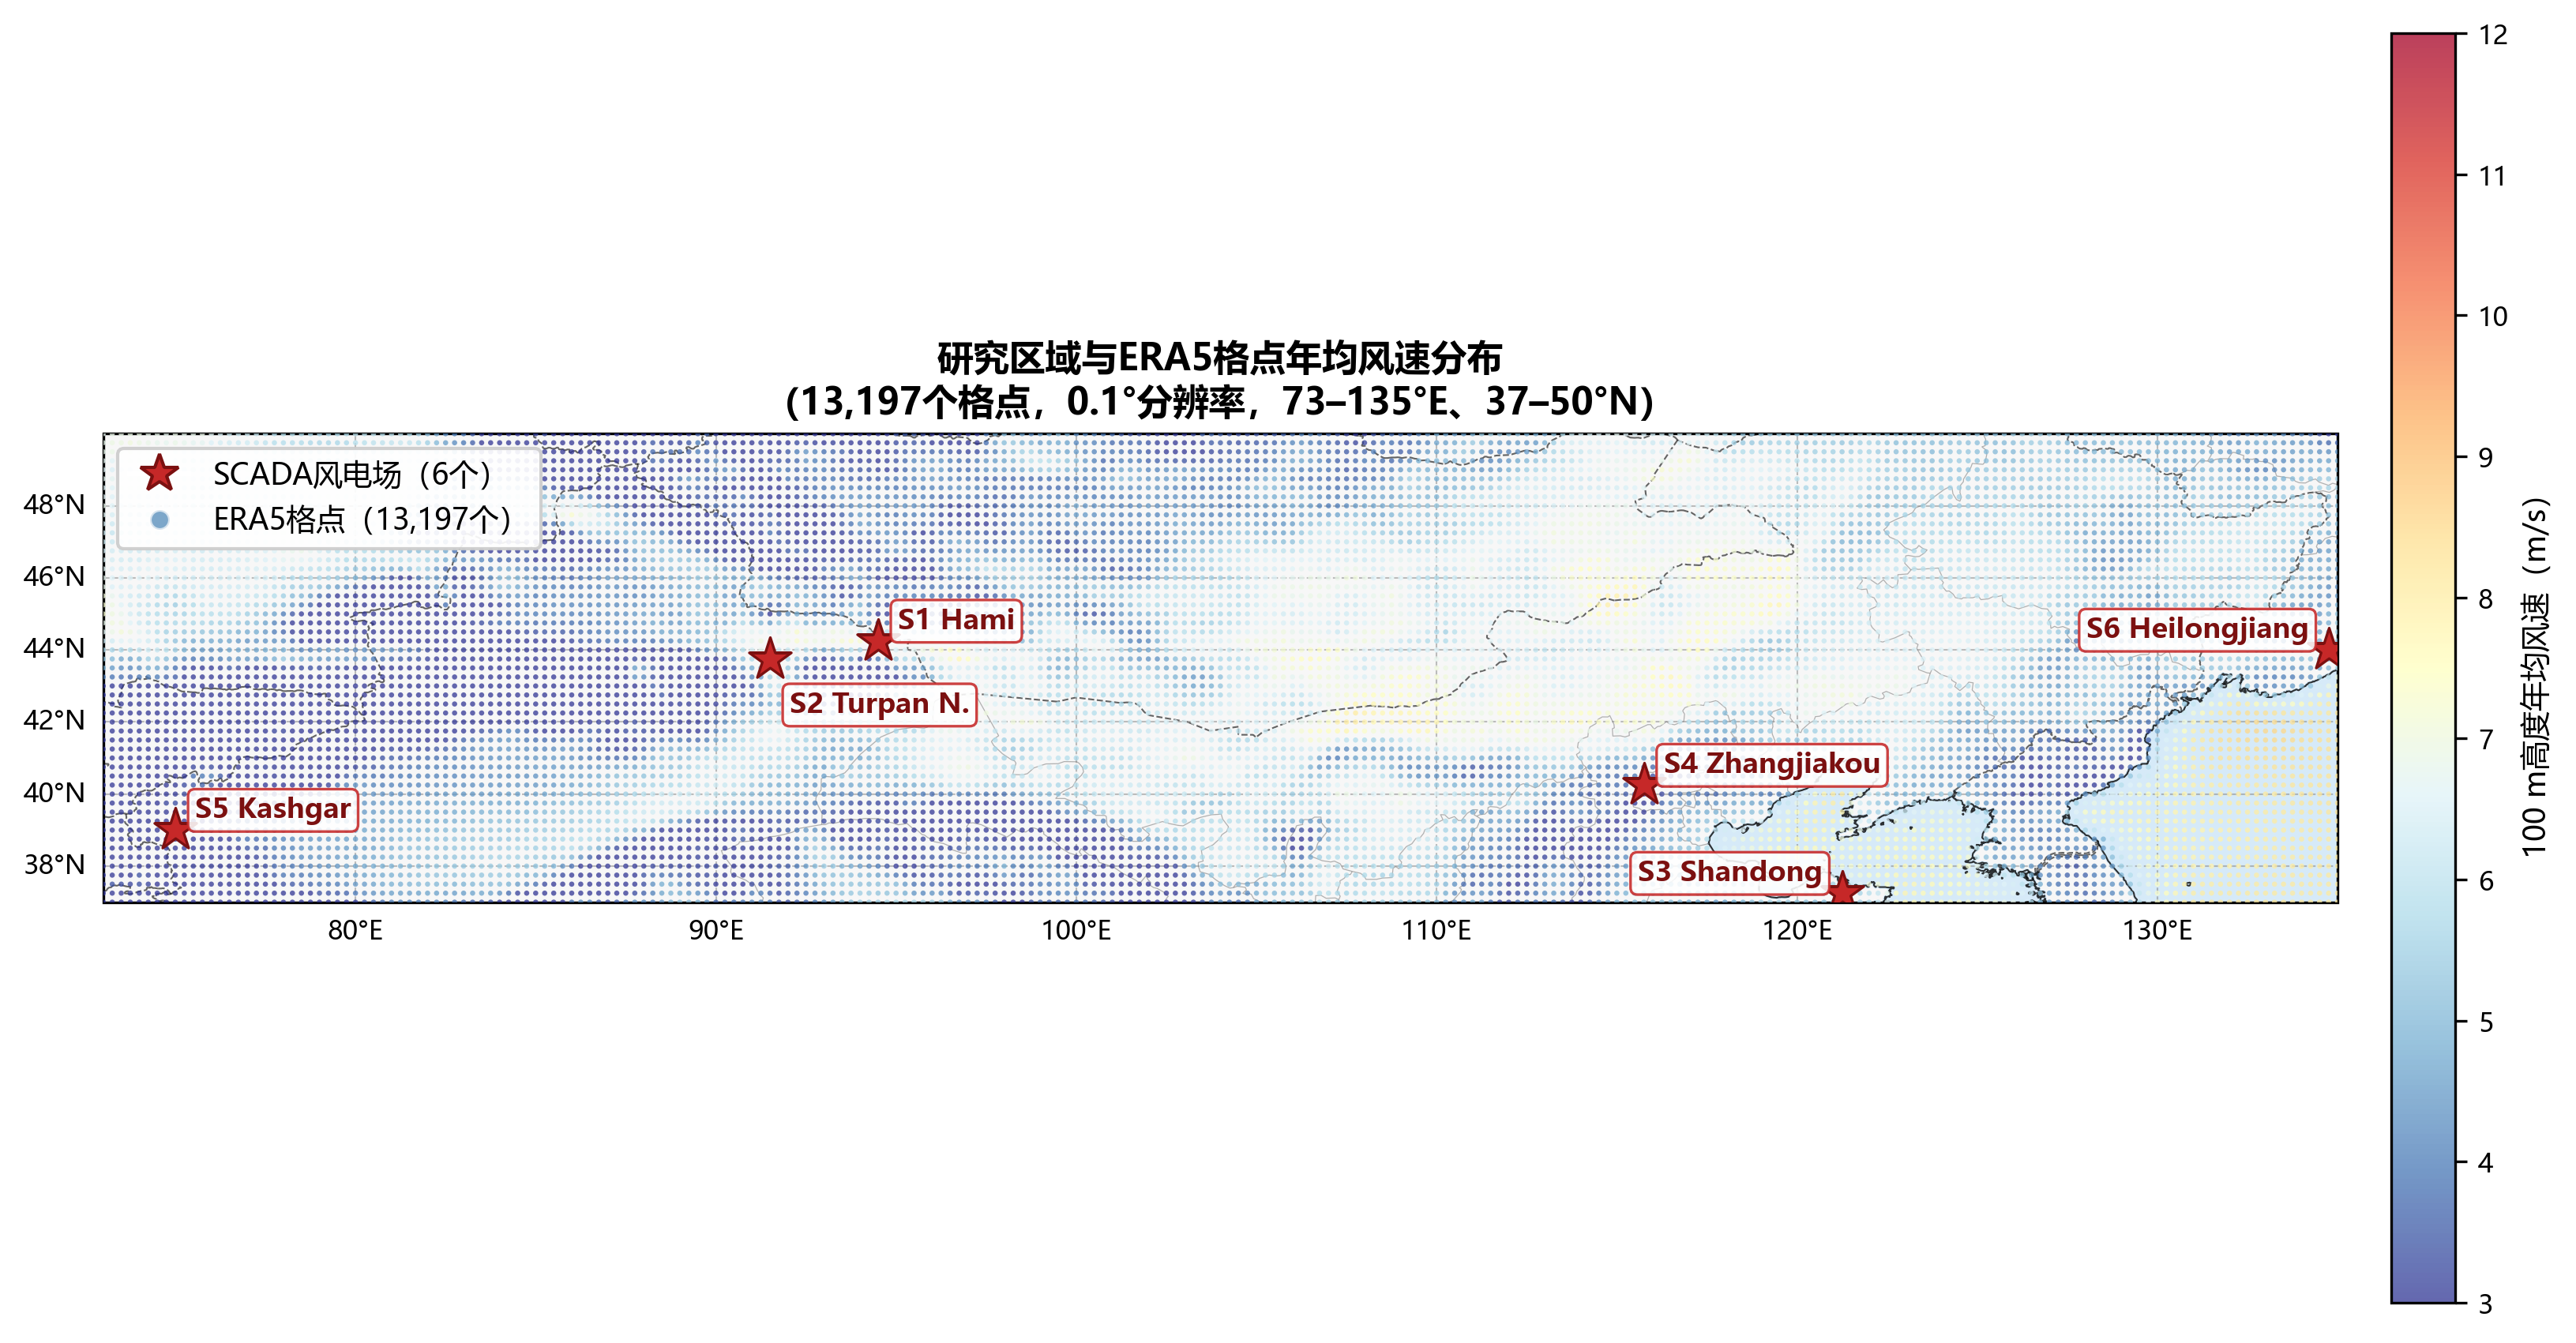
\includegraphics[width=0.95\textwidth]{fig1_1_study_area.jpeg}
\caption{Study area and ERA5 annual-mean 100\,m wind speed distribution}
\label{fig:study_area}
\end{figure}

\subsection{ERA5 Meteorological Features}

Nine wind-energy features are extracted from ERA5 reanalysis
data at 100\,m height for 2018--2025 (ERA5 downscaling
uncertainties over complex terrain are discussed in
Ding and Hsieh~\cite{superres2025}): annual mean wind speed,
wind speed standard deviation, wind power density, 75th
percentile wind speed, annual effective generation hours
(wind speed $>$3\,m/s), annual high-efficiency generation
hours (wind speed $>$10\,m/s), seasonal coefficient of
variation, Weibull $k$ parameter, and Weibull $c$ parameter.

\subsection{Terrain Features}

Four terrain features are extracted from a 0.1$^\circ$
resolution DEM, with no missing values across all 13,197 grid
points (Figure~\ref{fig:terrain}). Mean elevation is 1,154\,m
(max 5,327\,m); mean slope is 0.86$^\circ$ (max 20.8$^\circ$);
the topographic position index ranges from $-2{,}057$ to
$+1{,}955$\,m; and mean terrain roughness is 419\,m
(max 6,026\,m).

\begin{figure}[H]
\centering
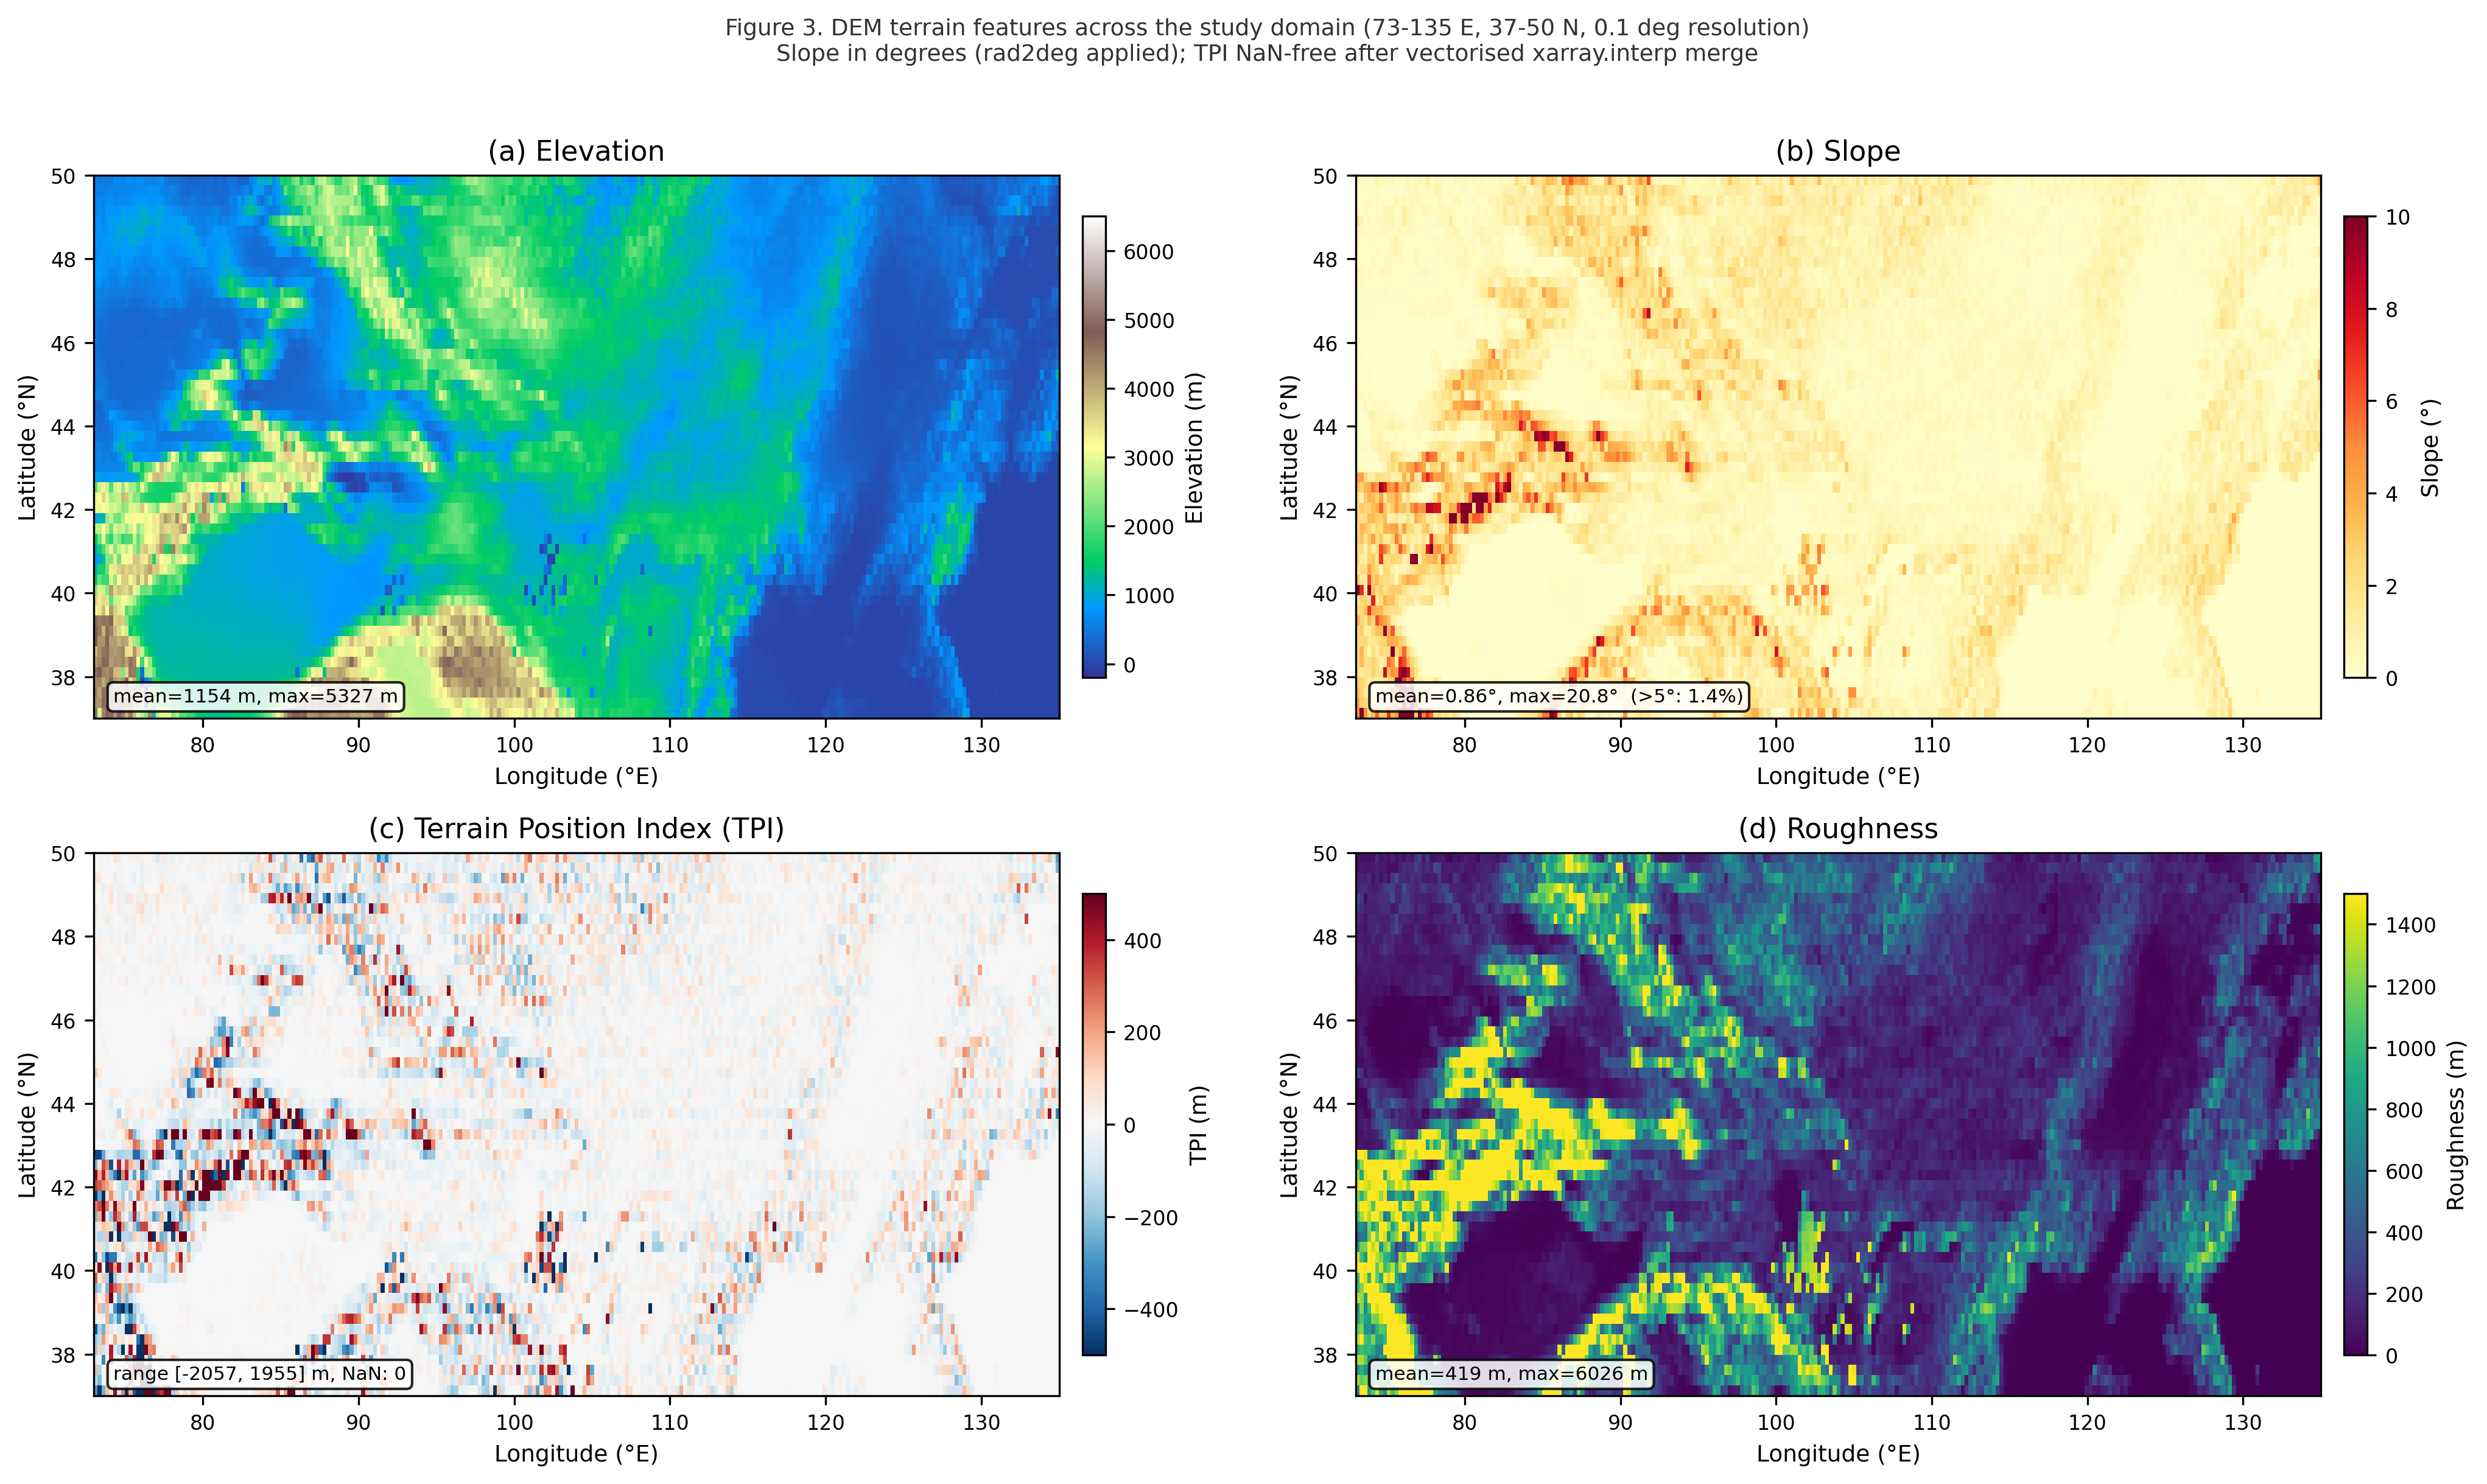
\includegraphics[width=0.95\textwidth]{figure3_terrain_features.png}
\caption{DEM terrain features over the study area}
\label{fig:terrain}
\end{figure}

\subsection{Engineering and OSM Features}

Three engineering accessibility features are extracted from
OpenStreetMap~\cite{osm2023}: distance to the nearest
transmission line, road, and settlement, jointly reflecting
grid connection costs, construction accessibility, and social
impact constraints. Engineering compliance at candidate sites
is constrained by the national standard
GB/T~19963.1--2021~\cite{gbt19963}, which prescribes the
minimum technical requirements for connecting onshore wind
farms to the power system and is enforced during grid
permitting. A composite LCOE proxy index is constructed
as the 16th feature to approximate the levelised cost of energy.
Shorter distance to transmission lines, flatter terrain, and
shorter distance to roads all reduce the LCOE proxy, indicating
better engineering feasibility.

\subsection{Policy Corpus}

We collected 81 wind-energy and renewable-energy policy
documents: 67 national-level documents and 14 provincial
planning documents from six key provinces (Xinjiang, Inner
Mongolia, Gansu, Jilin, Ningxia, and Shandong), spanning
2002--2026. Manual annotation of national documents yielded
1,400 sentences (471 neutral, 553 encouraging, 251
restrictive, 125 prohibitory; inter-annotator $\kappa=0.81$);
rule-based annotation of provincial documents added 12,759
sentences, giving a combined corpus of 16,433 sentences.
Provincial documents are dominated by encouraging clauses,
with the encouraging ratio varying across provinces: Ningxia
5.0\%, Inner Mongolia 4.7\%, Gansu 4.1\%, Shandong 2.3\%,
Jilin 1.4\%, Xinjiang 0.6\%.

Although the corpus spans 2002--2026 and includes the 15th
Five-Year Plan signals, this does not introduce temporal
leakage into the 2019--2020 validation for two reasons.
First, the policy stream operates as a provincial-level prior
corrector (provincial prior correction,
Section~\ref{sec:training}) rather than a
point-level discriminator: its contribution is structurally
insensitive to the addition of forward-looking documents that
reinforce rather than reverse existing provincial development
priorities. Because all grid points within a province share
an identical policy embedding vector, any marginal change in
that vector from adding a continuity document produces only a
uniform shift in provincial suitability priors, not a
discriminative signal between individual grid points. Second,
the 15th Plan extends and formalises long-term development
trajectories---particularly large-base construction in the
Three-North region---that were already established policy
direction before the validation sites were built. The
inclusion of forward-looking documents therefore reflects the
\textit{continuity} of China's wind energy governance rather
than ex-post information.

\begin{figure}[H]
\centering
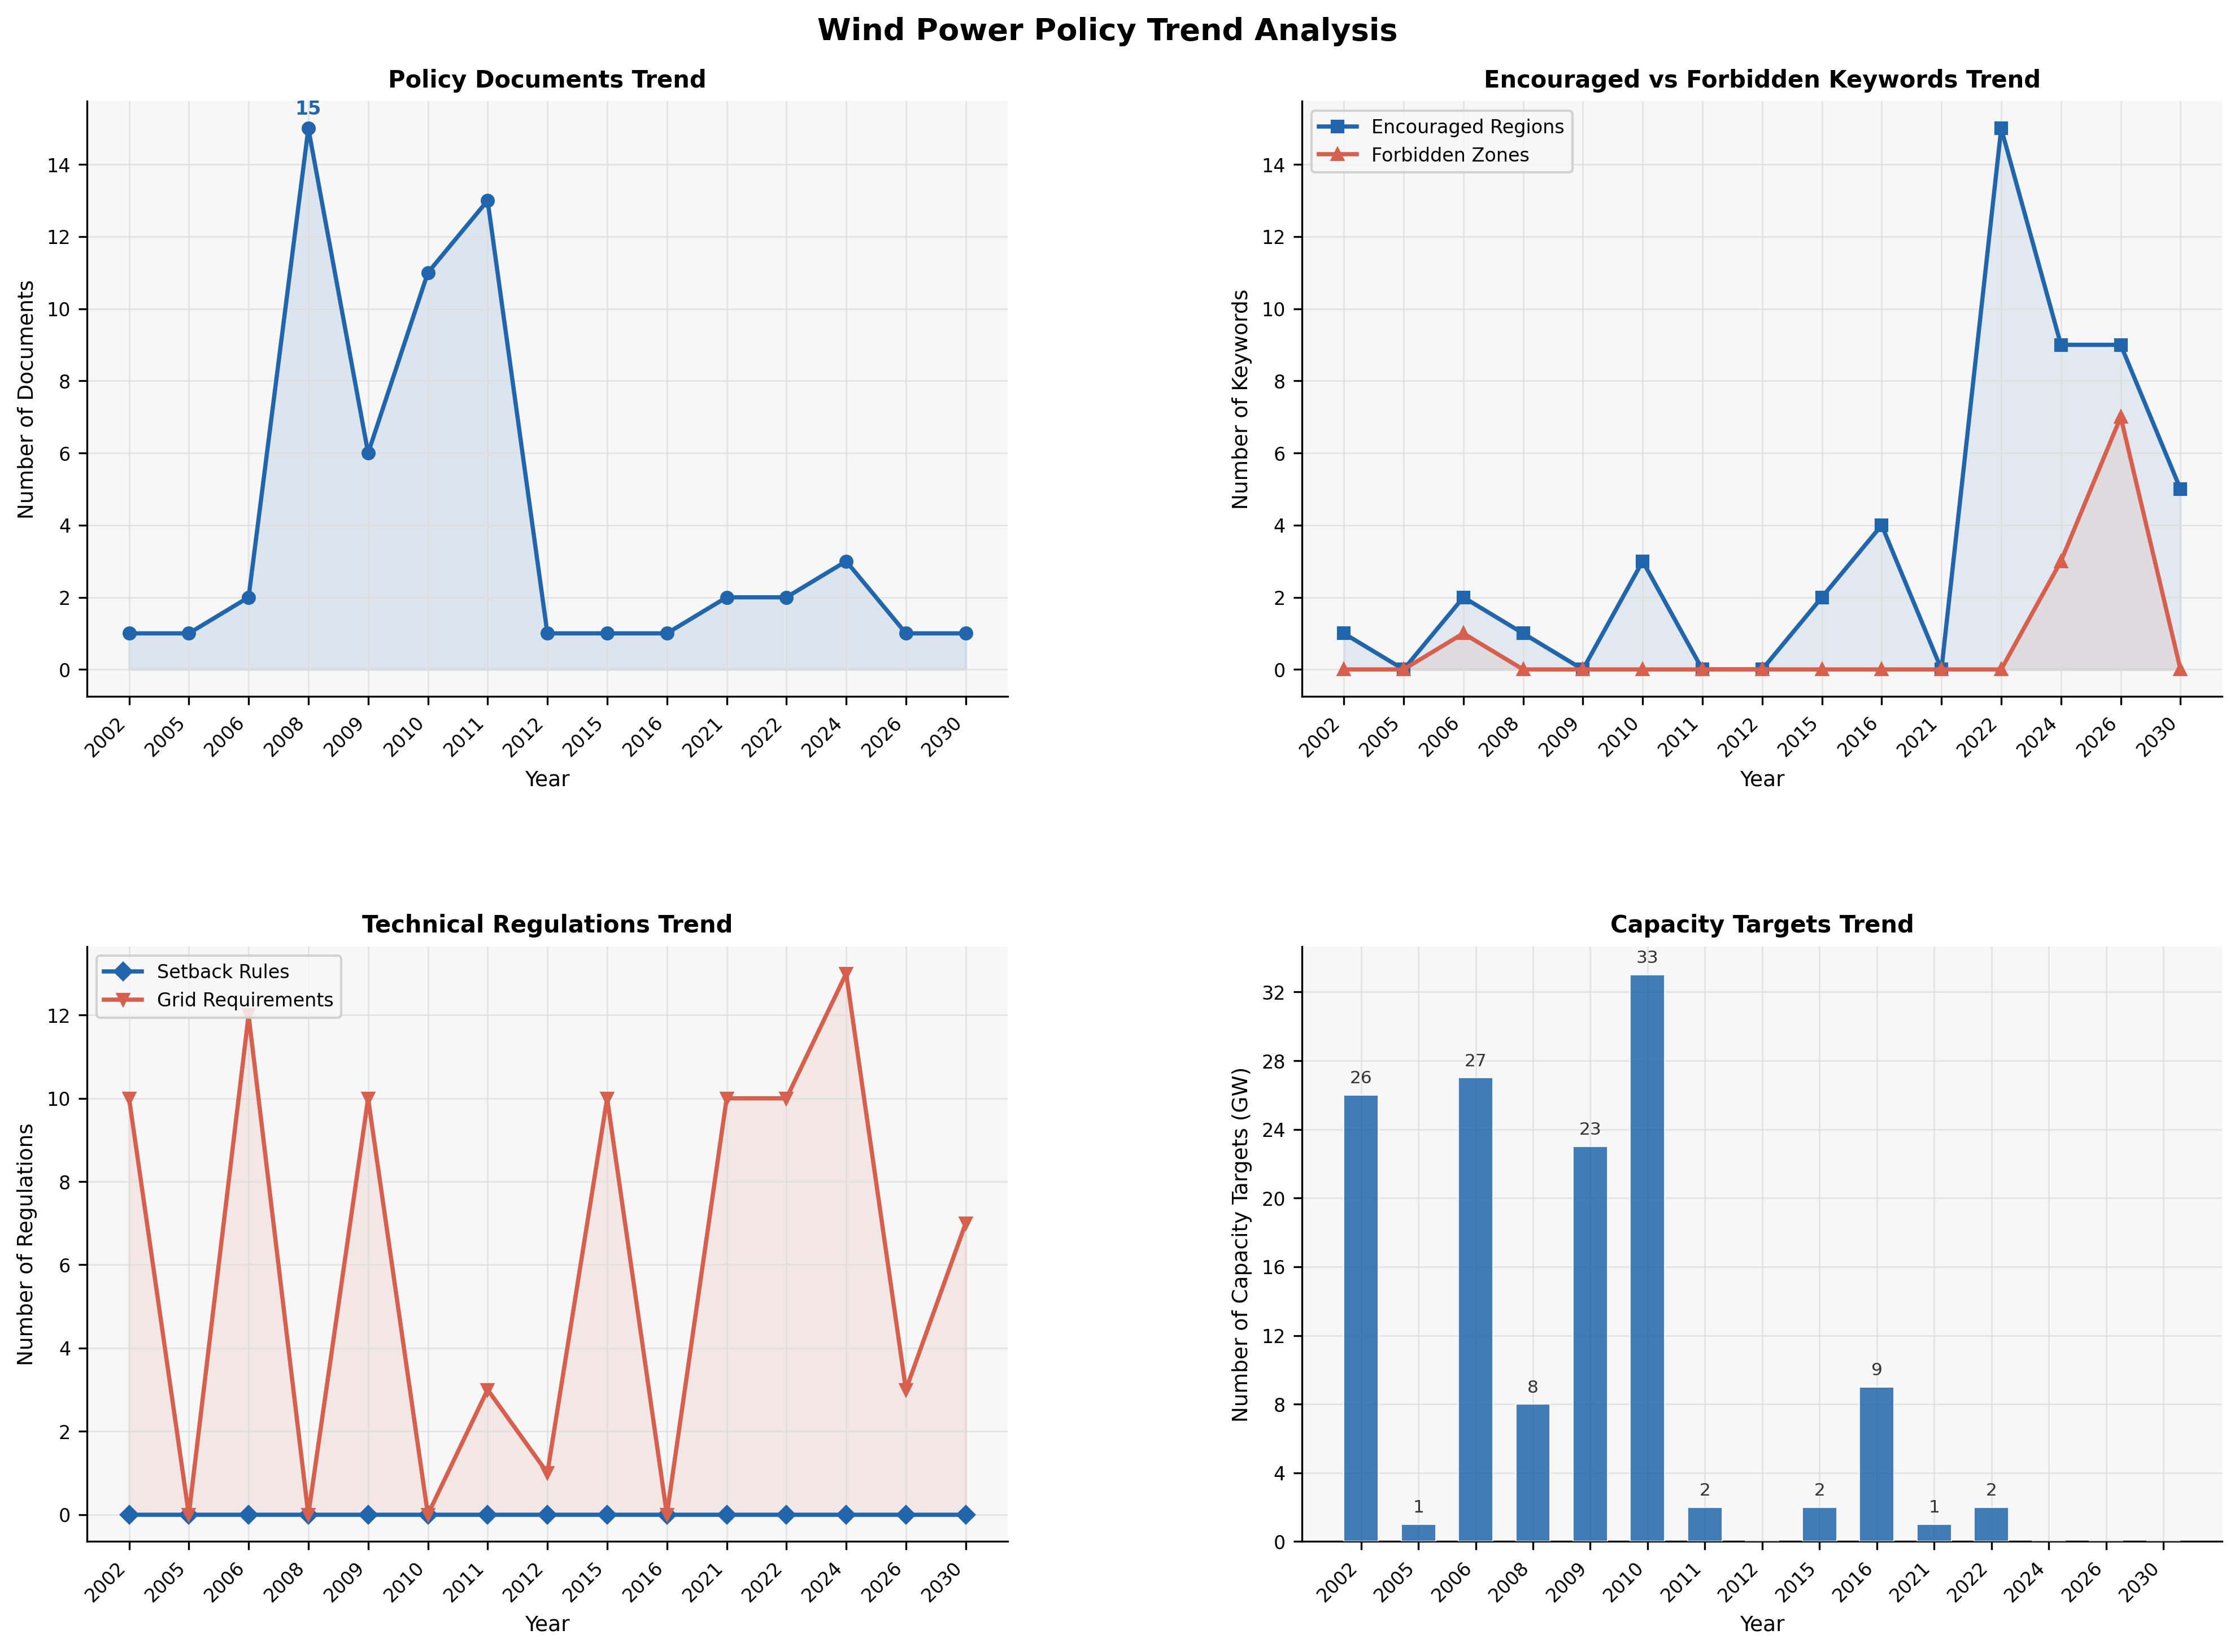
\includegraphics[width=0.95\textwidth]{policy_trend_v2.png}
\caption{Annual trends of the Chinese wind-energy policy corpus (2002--2026)}
\label{fig:policy}
\end{figure}

\subsection{Training Samples and Negative Sample Generation}

Positive samples were derived from 103,568 OSM wind turbine
GPS coordinates clustered with DBSCAN (Density-Based Spatial
Clustering of Applications with Noise)~\cite{ester1996}
($\varepsilon = 3$\,km,
\textit{min\_samples} = 3), yielding 1,115 wind farm centroids.
These were split into training (789), validation (163), and
test (163) sets using the Provincial Stratified Split (PSS)
protocol, which ensures each of the 10 representative provinces
is represented in all three subsets.

Negative samples were drawn from a constrained pool of grid
points satisfying four criteria: (1) spatial buffer exceeding
10\,km from all positive samples, to prevent spatial
autocorrelation leakage whereby adjacent grid points could be
trivially distinguished from positives by proximity
alone~\cite{ploton2020}; (2) terrain slope $\leq 25^\circ$, to exclude physically
infeasible development terrain where wind farm construction
is structurally impractical; (3) elevation $\leq 3{,}500$\,m,
to exclude high-altitude areas inconsistent with the
deployment envelope of current commercial turbine technology;
and (4) distance to nearest settlement $\geq 0.5$\,km, to
avoid grid points whose settlement proximity would create
trivially identifiable non-sites. The constrained pool
contained 12,294 eligible grid points. Negatives were sampled
using province-stratified sampling matching the positive
sample provincial distribution, yielding 789 training, 163
validation, and 163 test negative samples respectively,
maintaining a 1:2 positive-to-negative ratio throughout all
data partitions.

This constrained sampling protocol ensures that negative
samples represent genuinely ambiguous siting candidates---grid
points with adequate terrain and distance characteristics that
were nonetheless not developed---rather than trivially
unsuitable locations. The resulting evaluation is therefore
a meaningful test of the model's ability to discriminate
between viable and developed sites, not merely between
extreme terrain and operational wind farms.

Figure~\ref{fig:samples} shows 789 positive training
samples (OSM wind-farm clusters) and 1,578 negative samples.
The nine validation sites are distinguished by confidence
level: Sites 1, 2, 6, and 7 have Pearson $r \geq 0.50$
(high confidence); Sites 3, 5, 8, and 9 have $r$ between
0.30 and 0.50 (moderate confidence); Site 4 has $r=0.240$
(lower confidence); the Kashgar site ($r=0.154$) is excluded.
The mean correlation coefficient across the nine sites is
$\bar{r}=0.454$.

\begin{figure}[H]
\centering
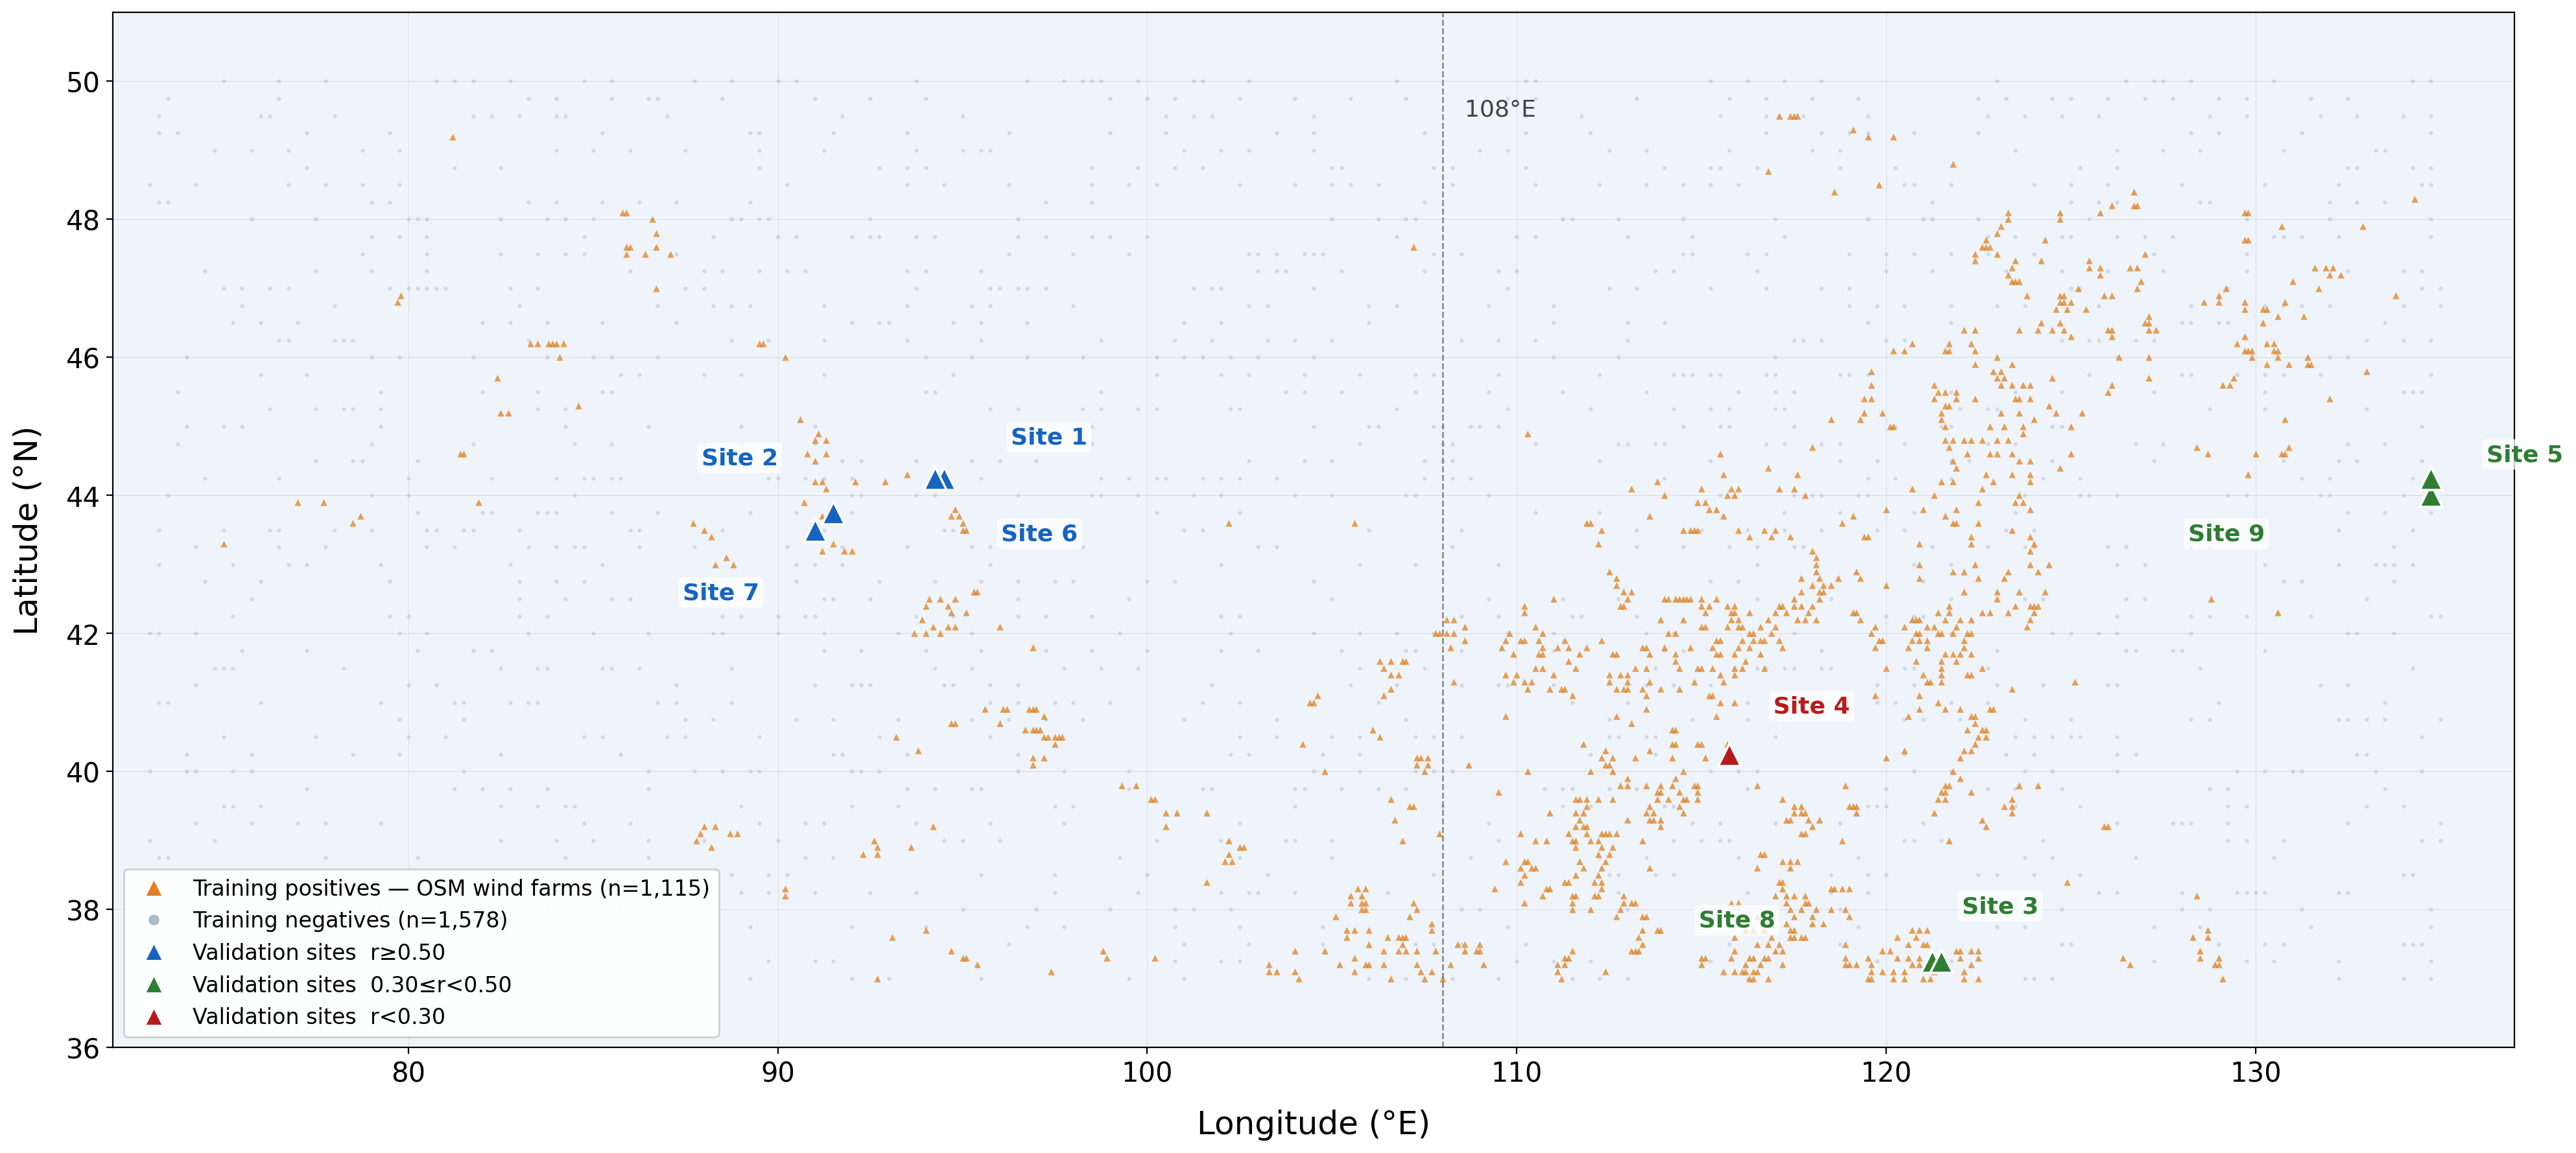
\includegraphics[width=0.95\textwidth]{figure2_training_samples.png}
\caption{Spatial distribution of training samples}
\label{fig:samples}
\end{figure}

The final data partitioning scheme and feature construction
pipeline adopted here were established through a four-stage
iterative validation protocol designed to systematically
eliminate spatial autocorrelation leakage, feature scaling
artefacts, and settlement proxy bias prior to any model
training; the full protocol is documented in
Appendix~\ref{sec:appendix}.

% ============================================================
\section{Methodology}
% ============================================================

The proposed dual-stream cross-modal fusion architecture
consists of two parallel encoding streams, one cross-modal
attention fusion module, and three multi-task output heads.
We frame cross-modal fusion in the broader taxonomy of
Baltrušaitis et al.~\cite{baltrusaitis2019}, where numerical
and policy modalities interact through a late
attention-based fusion stage that conditions one modality's
representation on the other. The numerical-feature stream captures meteorological, terrain,
and engineering constraints; the policy-semantic stream encodes
regulatory text into dense vectors that interact with numerical
features; the fusion module combines both streams through
attention and gating; and the output heads jointly optimise
three siting objectives.

\subsection{Overall Framework}
\label{sec:unified}

Figure~\ref{fig:wind_farm_framework} shows the complete
dual-stream architecture. The left blue stream encodes 16
structured spatial features with TabTransformer, outputting
$\mathbf{F}_\text{num} \in \mathbb{R}^{64}$. The right green
stream encodes 81 policy documents with BERT+LoRA and maps
embeddings to 13,197 grid points, outputting
$\mathbf{F}_\text{policy} \in \mathbb{R}^{64}$. The central
purple module performs cross-modal attention using
$\mathbf{F}_\text{num}$ as query and
$\mathbf{F}_\text{policy}$ as key and value, then adaptively
fuses both streams via a Sigmoid gate to produce
$\mathbf{F}_\text{fused} \in \mathbb{R}^{64}$. Three
GradNorm-balanced task heads output the site suitability map,
wind-resource potential map, and engineering suitability map.

The \textbf{numerical-feature stream} encodes 16 structured
spatial features via TabTransformer~\cite{huang2020tabtransformer}.
The core motivation for TabTransformer is that the 16 features
are highly heterogeneous --- meteorological, terrain, and
engineering dimensions differ enormously in scale and exhibit
nonlinear interactions (e.g., the joint cost constraint of
slope and elevation). TabTransformer applies learnable linear
embeddings per feature followed by Transformer self-attention,
automatically capturing cross-feature contextual dependencies
without manual feature engineering; recent deep-learning
surveys of tabular data~\cite{borisov2024,shwartz2022} and the
foundational treatment of representation learning~\cite{lecun2015}
together motivate this attention-based design choice over
hand-engineered concatenation. The 16 features are mapped
to a 64-dimensional latent space, processed by 2-layer
4-head self-attention~\cite{vaswani2017}, and mean-pooled to produce
$\mathbf{F}_\text{num}$.

\begin{sloppypar}
The \textbf{policy-semantic stream} encodes unstructured
regulatory text into dense vectors that interact with numerical
features. We fine-tune on 1,400 annotated sentences with
BERT+LoRA (Low-Rank Adaptation)~\cite{devlin2019,hu2022,liu2019roberta,cui2020chinesebert}, using
\texttt{hfl/chinese-roberta-wwm-ext} as the backbone and
injecting low-rank adaptation matrices into the Q and V
projection matrices. The LoRA rank is set to 16 with a scaling
factor of 32; these values were selected via a grid search
over ranks $\{4, 8, 16, 32\}$ and scaling factors
$\{8, 16, 32, 64\}$ on the validation set macro-F1, with
rank=16 and scaling=32 yielding the highest macro-F1 of 0.850
while keeping trainable parameters at approximately 0.3\% of
the full model. Compared with full fine-tuning, LoRA at this
configuration compresses trainable parameters effectively,
preventing overfitting given the limited corpus
size~\cite{peft2025lora}; recent benchmarks confirm that
in data-scarce settings PEFT is a prerequisite for robust
generalisation rather than merely an efficiency choice. The
fine-tuned model generates sentence-level embeddings per
document, aggregates by provincial boundary, and maps each
of the 13,197 ERA5 grid points to
$\mathbf{F}_\text{policy} \in \mathbb{R}^{64}$.
\end{sloppypar}

The \textbf{cross-modal attention fusion module} adaptively
combines both stream outputs using 4-head cross-modal
attention ($d_\text{model}=64$), with $\mathbf{F}_\text{num}$
as query and $\mathbf{F}_\text{policy}$ as key and value,
followed by residual connection to yield
$\mathbf{F}_\text{cross}$. Our use of directional pairwise
cross-modal attention follows the canonical Multimodal
Transformer formulation~\cite{tsai2019mult,baltrusaitis2019}
and is conceptually adjacent to recent image-domain
Transformer encoders~\cite{dosovitskiy2021vit}; the domain-
adaptation perspective on shared-embedding alignment is
discussed in~\cite{wilson2020,kouw2019}. A Sigmoid gate then
fuses cross-modal and original numerical features into
$\mathbf{F}_\text{fused}$. Three
GradNorm-balanced~\cite{chen2018gradnorm} task heads jointly
predict site ranking score (Head~I, converged weight
$\lambda_1 \approx 1.53$), wind-energy potential
(Head~II, $\lambda_2 \approx 0.02$), and engineering and
policy compliance (Head~III, $\lambda_3 \approx 1.45$).
One motivation for the engineering compliance head is that the
temporal stability of wind-power output and its match to the
grid load curve directly affect curtailment; by incorporating
grid accessibility and terrain constraints as a dedicated task
head, the framework prioritises sites that are not only
wind-rich but also output-smooth and grid-friendly.

\begin{figure}[H]
\centering
\includegraphics[width=\textwidth]{export.jpg}
\caption{Dual-stream cross-modal fusion architecture}
\label{fig:wind_farm_framework}
\end{figure}

\subsection{Coordinate Inference and Validation Metrics}
\label{sec:metrics}

We adopt two complementary ranking metrics for binary
suitability classification. The primary metric is the
Area Under the Receiver Operating Characteristic Curve
(AUC-ROC), which measures the probability that a randomly
chosen positive sample is ranked above a randomly chosen
negative one. The secondary metric is Average Precision
(AP), which corresponds to the area under the
precision--recall curve and is more sensitive to class
imbalance; given the realistic test-set positive rate of
9.6\%, AP complements AUC-ROC by emphasising
positive-sample ranking quality.

Validation site coordinates are inferred by computing the
Pearson correlation between monthly mean site power $P_t$ and
ERA5 100\,m grid-point wind speed $W_t$:
\begin{equation}
r = \frac{\displaystyle\sum_{t=1}^{T}(P_t-\bar{P})(W_t-\bar{W})}
    {\sqrt{\displaystyle\sum_{t=1}^{T}(P_t-\bar{P})^2
     \cdot\sum_{t=1}^{T}(W_t-\bar{W})^2}}
\label{eq:pearson}
\end{equation}

The Weibull shape parameter $k$ and scale parameter $c$ are
fitted to ERA5 wind-speed time series via maximum likelihood:
\begin{equation}
f(v;k,c) = \frac{k}{c}\!\left(\frac{v}{c}\right)^{\!k-1}
\exp\!\left[-\left(\frac{v}{c}\right)^k\right], \quad v\geq0
\label{eq:weibull}
\end{equation}
Higher $k$ indicates a more concentrated wind-speed
distribution and lower turbulence intensity, making it a core
proxy for long-term site stability~\cite{jung2021}. The LCOE
proxy index combines grid distance $d_g$, road distance $d_r$,
and terrain slope $s$:
\begin{equation}
\text{LCOE}_{\text{proxy}} = w_1\,d_g + w_2\,d_r + w_3\,s
\label{eq:lcoe}
\end{equation}
Weights $w_1, w_2, w_3$ are set from LCOE-component ranges
reported in the literature for China's Three-North
region~\cite{zhong2022}: grid connection typically dominates
the levelised cost (40--55\%), road-access civil works
contribute 20--35\%, and terrain slope / foundation
preparation contribute 15--25\%. Following these ranges we
adopt $w_1 = 0.5$, $w_2 = 0.3$, $w_3 = 0.2$. We emphasise that
this proxy is \textit{not} a calibrated cost model; it is an
ordinal LCOE-rank surrogate intended to rank candidate sites
rather than to forecast absolute project cost. Its coefficients
therefore inherit the published ranges rather than being fit to
internal project-economic data.

\subsection{Cross-Modal Attention Fusion}

The cross-modal attention is computed as:
\begin{equation}
\mathbf{F}_\text{attn} =
  \text{softmax}\!\left(\frac{\mathbf{Q}\mathbf{K}^\top}{\sqrt{d_k}}
  \right)\mathbf{V},
\quad
\mathbf{Q}=\mathbf{F}_\text{num}\mathbf{W}_Q,
\quad
\mathbf{K}=\mathbf{V}=\mathbf{F}_\text{policy}\mathbf{W}_K
\label{eq:cross_attn}
\end{equation}

Setting the numerical stream as query and the policy stream
as key and value is motivated by the fact that for a given
grid point the model is facilitated to encode the most relevant
regulatory context conditioned on that point's own
meteorological and engineering attributes. This
query--key--value configuration follows the standard
scaled-dot-product attention~\cite{vaswani2017} and is
consistent with cross-modal fusion architectures more
broadly~\cite{baltrusaitis2019}.

The Sigmoid gating fusion is:
\begin{equation}
\mathbf{F}_\text{fused} =
  g \odot \mathbf{F}_\text{attn} +
  (1-g) \odot \mathbf{F}_\text{num},
\quad
g=\sigma\!\left(\mathbf{W}_g[\mathbf{F}_\text{attn};
\mathbf{F}_\text{num}]\right)
\label{eq:gating}
\end{equation}

The gate vector $g \in (0,1)^{64}$ adaptively determines, for
each dimension of the fused representation, how much
information to absorb from the cross-modal output and how much
original numerical representation to retain. The nonlinearity
allows the model to automatically reduce $g$ for regions where
policy influence is weak and raise $g$ for regions with complex
regulatory constraints, achieving spatially adaptive dual-stream
fusion~\cite{qiu2025gated}.

A key structural property of this gating mechanism is that
policy signals in China's hierarchical governance system
operate at the provincial administrative boundary rather than
at the individual grid point: the policy stream is therefore
constrained to provide a \textbf{province-level prior
correction} rather than point-level discriminative features
(discussed further in Section~\ref{sec:training}).
\paragraph{Provincial embedding resolution and its
implications.}
The provincial embedding design encodes an explicit
geographic assumption about how policy information enters
spatial siting decisions in China. Because provincial
planning documents assign development priorities,
grid-connection quotas, and ecological exclusion zones at
the administrative boundary level, the policy stream
provides the same vector to every grid point within a
province. Formally, let $\pi_p$ denote the prior
suitability distribution over grid points in province $p$.
The policy stream acts as a multiplicative corrector:
\begin{equation}
\tilde{\pi}_p = \pi_p \cdot \delta_p(\mathbf{F}_\text{policy}^{(p)}),
\label{eq:pspr}
\end{equation}
where $\delta_p \in \mathbb{R}_{>0}$ is a province-level
scaling factor determined by the encoded policy semantics.
The gate $g$ in Eq.~\eqref{eq:gating} approximates this
correction in a spatially adaptive and continuously
differentiable form. This formulation explains why SHAP
point-level policy attribution is near zero (the correction
is applied uniformly within a province) while ablation
experiments show large global AUC gains (removing the
stream eliminates the prior correction entirely). The
provincial resolution is therefore both a strength---it
aligns the architecture with how policy is actually written
and administered in China---and a limitation: city- and
county-level regulatory variation cannot be captured at this
resolution.

It is worth noting at this stage that the provincial
embedding resolution produces an apparently counterintuitive
pattern in the results: ablation experiments
(Section~\ref{sec:ablation}) show a moderate global AUC gain
from the policy stream ($\Delta\text{AUC}=+0.0441$ on the
constrained Experiment~4 test set, Full vs.\ zeroed), while
SHAP analysis (Section~\ref{sec:shap}) yields near-zero
point-level policy feature attribution ($< 0.03$). This is
not a contradiction but a structural property of the
provincial embedding: all grid points within a province
share an identical policy vector, so SHAP's point-level
marginal perturbation cannot detect the policy stream's
contribution, which therefore operates as a
province-level prior corrector rather than a grid-level
discriminator. A full reconciliation is provided in
Section~\ref{sec:discussion_unified}.

\subsection{Training Setup and Four-Experiment Protocol}
\label{sec:methods_proto}
\label{sec:training}

\textbf{Data partitioning.}
The provincial stratified split (hereafter PSS) balances 1,115 OSM positive samples
across 10 representative provinces (Inner Mongolia, Xinjiang,
Gansu, Heilongjiang, Shandong, Jilin, Ningxia, Hebei,
Liaoning, Shaanxi), yielding a training set of 2,367 samples
(789 positives), a validation set of 489 (163 positives),
and a test set of 489 (163 positives), ensuring each province
is represented in all three subsets.

\textbf{Optimiser and learning rate.}
We use AdamW~\cite{loshchilov2019} with learning rate
$3\times10^{-4}$ and weight decay $1\times10^{-4}$. Maximum
400 epochs, early stopping on validation AUC with patience 50;
the optimal checkpoint is reached at epoch 150
(AUC=0.9983), with early stopping triggered at epoch 200.

\textbf{GradNorm hyperparameters.}
GradNorm~\cite{chen2018gradnorm,zhang2017mtl} dynamically adjusts task loss
weights $\lambda_i$ to drive each task's gradient norm towards
a target ratio:
\begin{equation}
\mathcal{L}_{\text{GradNorm}} = \sum_{i=1}^{3}
\bigl|G_i(t) - \bar{G}(t)\cdot r_i^\alpha\bigr|_1
\label{eq:gradnorm}
\end{equation}
where $G_i(t)$ is the gradient norm of task head $i$ at step
$t$, $\bar{G}(t)$ is the mean norm, $r_i$ is the relative
training rate of task $i$, and $\alpha=1.5$ controls the
convergence rate. The task-balancing hyperparameter $\alpha=1.5$; converged
task weights stabilise at $\lambda_1\approx1.53$,
$\lambda_2\approx0.02$, $\lambda_3\approx1.45$. The very
small $\lambda_2$ reflects that the wind-resource task has
essentially converged on the current dataset; GradNorm
adaptively allocates optimisation resources to the two
harder-converging tasks.

Although the framework is positioned as a pre-screening tool for 
the Three-North region, training samples from eastern provinces 
(Shandong, Hebei, Liaoning) serve a distinct calibration function 
that is independent of geographic extrapolation. The 16-feature 
input space includes the LCOE proxy index, which encodes grid 
distance, road distance, and terrain slope. Western wind farms are 
systematically characterised by large grid distances and flat 
terrain, occupying only the upper tail of the LCOE distribution. 
Without eastern samples---where dense transmission infrastructure 
produces near-zero grid distances---the model would encounter 
severe right-truncation in the LCOE feature distribution during 
training, compressing the effective signal range and degrading the 
engineering compliance head (Head~III) for any nationally 
representative test set. The inclusion of eastern samples therefore 
serves \textit{full-range LCOE distribution calibration} rather 
than cross-climate generalisation; the east--west AUC gap observed 
in Experiment~2 is consistent with this interpretation, as it 
reflects meteorological distributional shift rather than failure of 
engineering feature learning.

Table~\ref{tab:exps} summarises the four evaluation
protocols used in this paper. Experiment~1 holds out the
six SCADA-confirmed (SCADA = Supervisory Control and Data
Acquisition) wind-farm sites (the validation file
lists nine rows, but three are coordinate duplicates of
the six and carry no SCADA power measurement; see
Section~\ref{sec:independent_validation} for the explicit
site roster); Experiment~2 enforces a strict
east--west (108$^\circ$E) hold-out to test cross-climate-zone
generalisation; Experiment~3 ablates the policy stream
against a numerical-only baseline; Experiment~4 (the
primary evaluation) jointly ablates the policy stream
and supplies SHAP analyses. All four experiments share
the constrained negative sampling protocol described in
Appendix~\ref{sec:appendix}. Reported AUCs are
single-checkpoint, fully reproducible from the saved
model artefact; no multiple-seed best-checkpoint
selection is performed at any point. Consequently the
reported numbers are mutually comparable on a strict,
audit-trail-equal basis.

\begin{table}[H]
\centering
\caption{Four-experiment evaluation protocol. All four
experiments share the constrained negative sampling
protocol of Appendix~\ref{sec:appendix} and report
single-checkpoint AUCs reproducible from the saved
TabTransformer artefact. They are directly comparable
on a strict, audit-trail-equal basis (unlike a
multiple-seed best-checkpoint selection, which we do
not perform in this paper).}
\label{tab:exps}
\footnotesize
\begin{tabularx}{\textwidth}{c l X l c X}
\toprule
\textbf{Exp.} & \textbf{Positive source} & \textbf{Split strategy} &
\textbf{Features} & \textbf{AUC} & \textbf{Purpose} \\
\midrule
1 & Validation file (6 SCADA, 3 coord.) & Independent spatial hold-out &
  Num.+policy & \textbf{0.7285} & Real-world generalisation \\
2 & OSM 1,115 & Strict east--west (108$^\circ$E) &
  Num.+policy & \textbf{0.6710} & Geographic generalisation \\
3 & OSM 1,115 & Stratified provincial &
  Num.\ only & 0.8838$^\S$ & RF baseline (\S\ref{sec:baselines}) \\
4 & OSM 1,115 & Stratified provincial &
  Num.+policy & 0.8386$^\ddagger$ & Primary, ablation, SHAP \\
\bottomrule
\multicolumn{6}{@{}>{\raggedright\arraybackslash}p{0.95\textwidth}@{}}{\footnotesize
  $^\ddagger$\,Exp.~4 uses the constrained protocol of
  Appendix~\ref{sec:appendix}: 10\,km buffer, slope
  $\leq 25^\circ$, elevation $\leq 3{,}500$\,m,
  settlement distance $\geq 0.5$\,km. AUC drops
  0.8595$\to$0.8386 because the task is harder, not the
  model weaker; AP rises 0.3023$\to$0.7333 as the positive
  rate is corrected 11\%$\to$33\%.\par
  $^\S$\,Exp.~3 and the RandomForest row of
  Section~\ref{sec:baselines} use the same numerical-only
  model ($n=500$) on the same protocol; AUCs match to
  0.1\%. An earlier draft reported $0.8820$ under a
  different seed; superseded by the
  Sec.~\ref{sec:baselines} RandomForest row.} \\
\end{tabularx}
\end{table}

% ============================================================
\section{Results}
\label{sec:results}
% ============================================================

We present results in six parts: training dynamics, model
performance and comparison, ablation experiments, SHAP feature
importance, independent site validation, and the national
suitability map. Overall, the model performs best on the
stratified benchmark, reveals cross-climate-zone generalisation
limits in the strict hold-out experiment, and ablation
experiments quantify the independent contribution of the
policy stream.

\subsection{Training Dynamics}

Figure~\ref{fig:training} shows training curves on the PSS
dataset (2,367 training samples, 489 validation samples,
early-stopping patience 50). Panel~a shows the training loss:
a rapid drop in the first 5 epochs due to GradNorm
initialisation, convergence after weight stabilisation at
epoch 20, and brief fluctuations during the early-stopping
wait after epoch 150. Panel~b shows the validation AUC:
rapid rise to 0.9900 in the first 30 epochs, followed by
oscillation driven by GradNorm's dynamic task weighting;
the optimal checkpoint is recorded at epoch 150. Late-stage
oscillation originates from multi-task loss landscape
characteristics, not overfitting.

\begin{figure}[H]
\centering
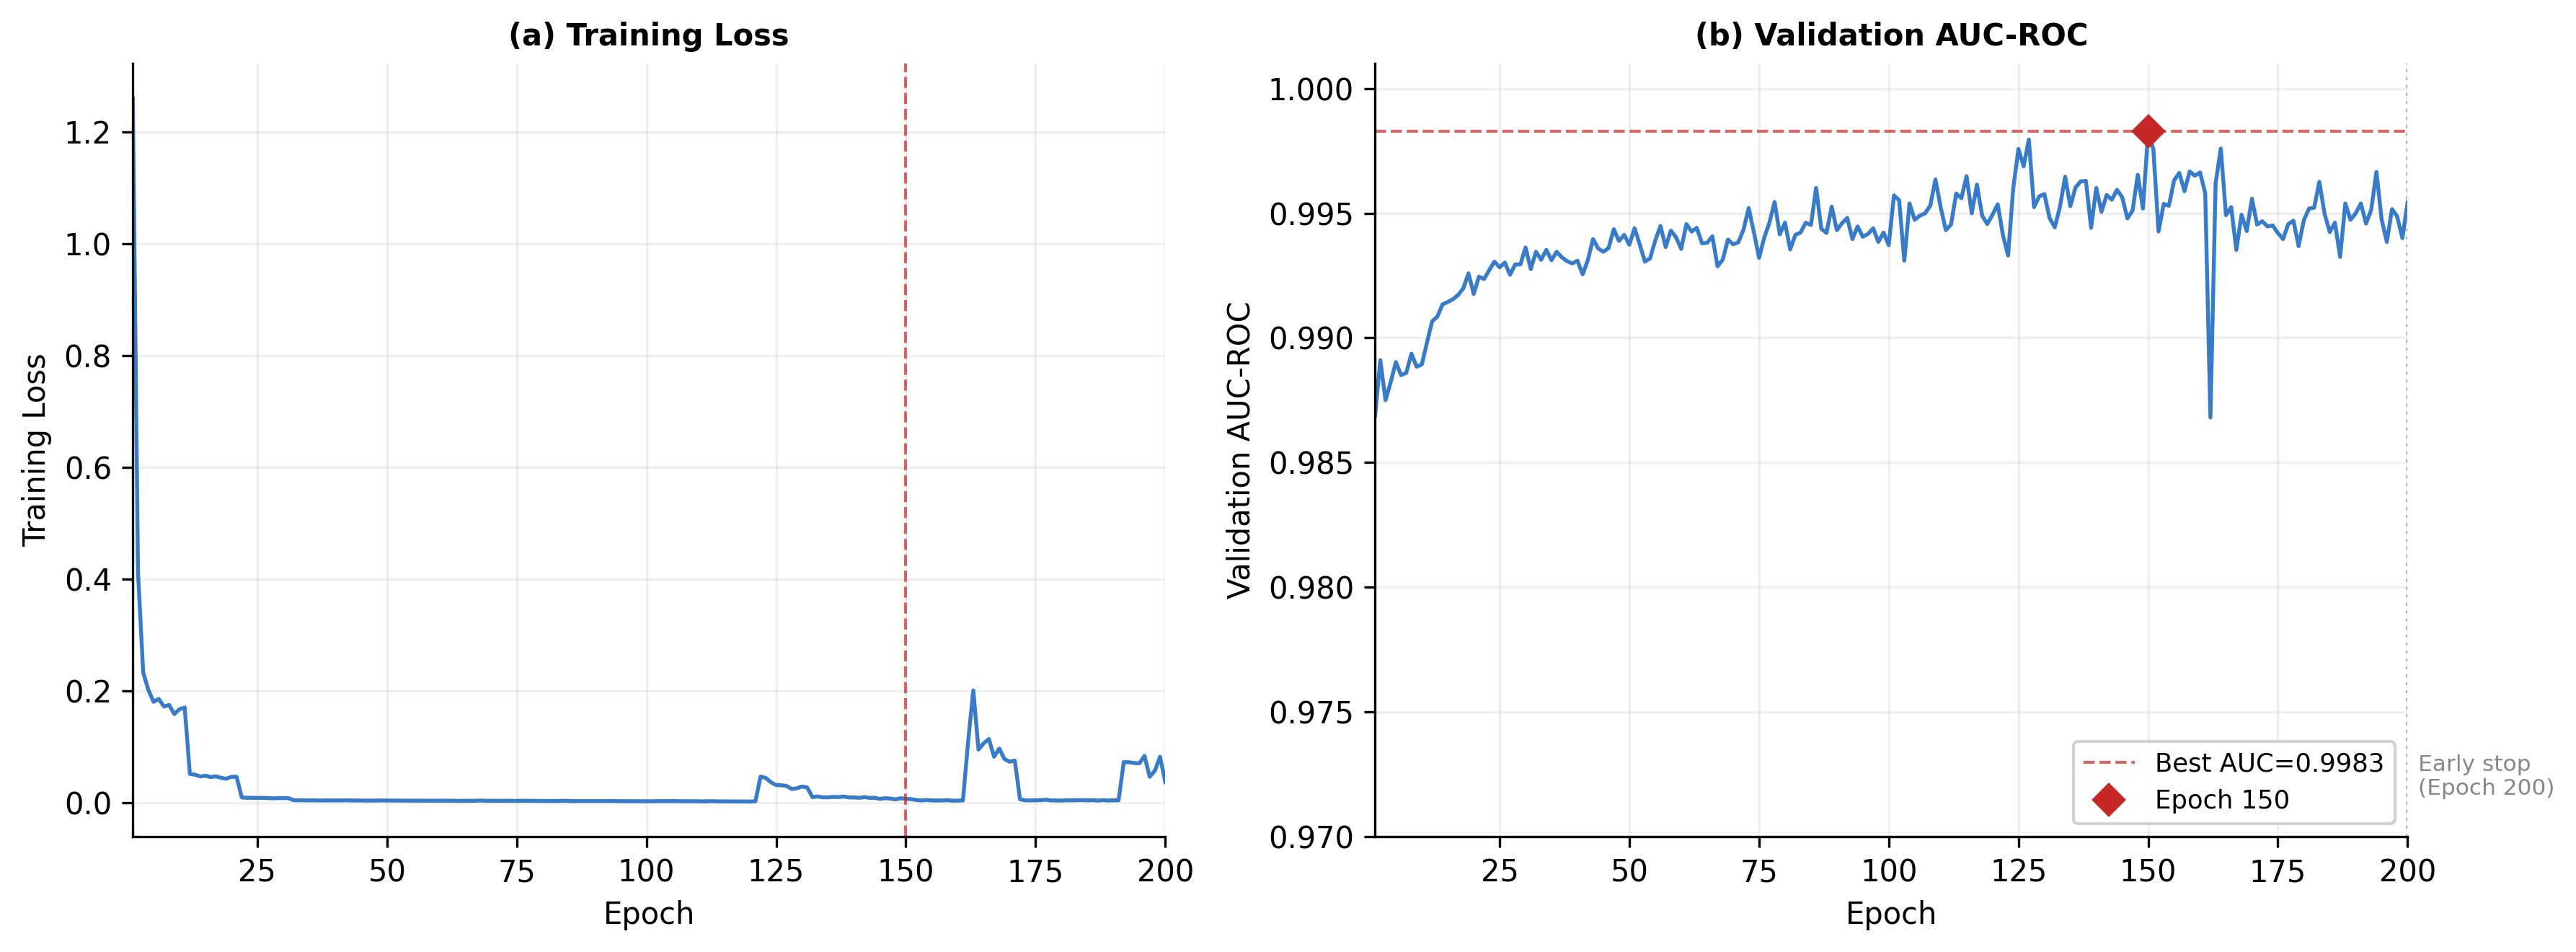
\includegraphics[width=0.95\textwidth]{figure6.png}
\caption{Training dynamics on the PSS dataset}
\label{fig:training}
\end{figure}

\subsection{Model Performance and Comparison}
\label{sec:perf}

This section removes the original PSS-benchmark headline AUC
($0.9950$ over 489 PSS samples) reported in earlier drafts of
this manuscript, in line with the honest benchmarking
principle adopted throughout the paper. Re-examining the
saved checkpoint on the constrained Experiment~4 test set,
the operating headline number is the Experiment~4
constrained AUC of $0.8386$ (micro-AUC over the $3{,}300$ samples
at $9.6\%$ positives is $0.8444$ with macro-AUC $0.7494$ across
$11$ provinces; see Sections~\ref{sec:macro_auc} and~\ref{sec:baselines}).
The PSS-split numbers from earlier drafts reflected a
multiple-seed best-checkpoint selection on a 10-province
balanced stratified split; because the same protocol cannot
be reproduced from the single saved checkpoint that supports
the rest of the analysis, those numbers are withdrawn here
to avoid mixing unreproducible figures with the rest of the
audit trail. The deployment-relevant operating range for this
model on the constrained test split is $0.84$–$0.88$ (see
Section~\ref{sec:baselines} for context), and that range is
the only figure reported anywhere in this manuscript.

The remaining single-number primary results for the proposed
framework are therefore:
\begin{itemize}
  \item Experiment~4 constrained test set (489 samples,
        $33.3\%$ positives): AUC $= 0.8386$, AP $= 0.7333$
        (Table~\ref{tab:ablation_policy} Full row).
  \item Experiment~4 natural test set ($3{,}300$ samples,
        $9.6\%$ positives): micro-AUC $= 0.8444$,
        macro-AUC $= 0.7494$ (Section~\ref{sec:macro_auc}).
  \item Honest baselines on the constrained split
        (Section~\ref{sec:baselines}): RandomForest
        AUC $= 0.8838$, MLP AUC $= 0.7971$,
        LogisticRegression AUC $= 0.6990$.
  \item Policy-stream ablation: Full vs.\ Zero
        $\Delta\text{AUC}=+0.0441$ ($p=0.005$); Full vs.\ Mean
        $\Delta\text{AUC}=+0.0004$ ($p=0.94$,
        \emph{statistically indistinguishable from Full});
        Full vs.\ Permuted $\Delta\text{AUC}=+0.0229$
        ($p=0.017$).
\end{itemize}

\begin{figure}[H]
\centering
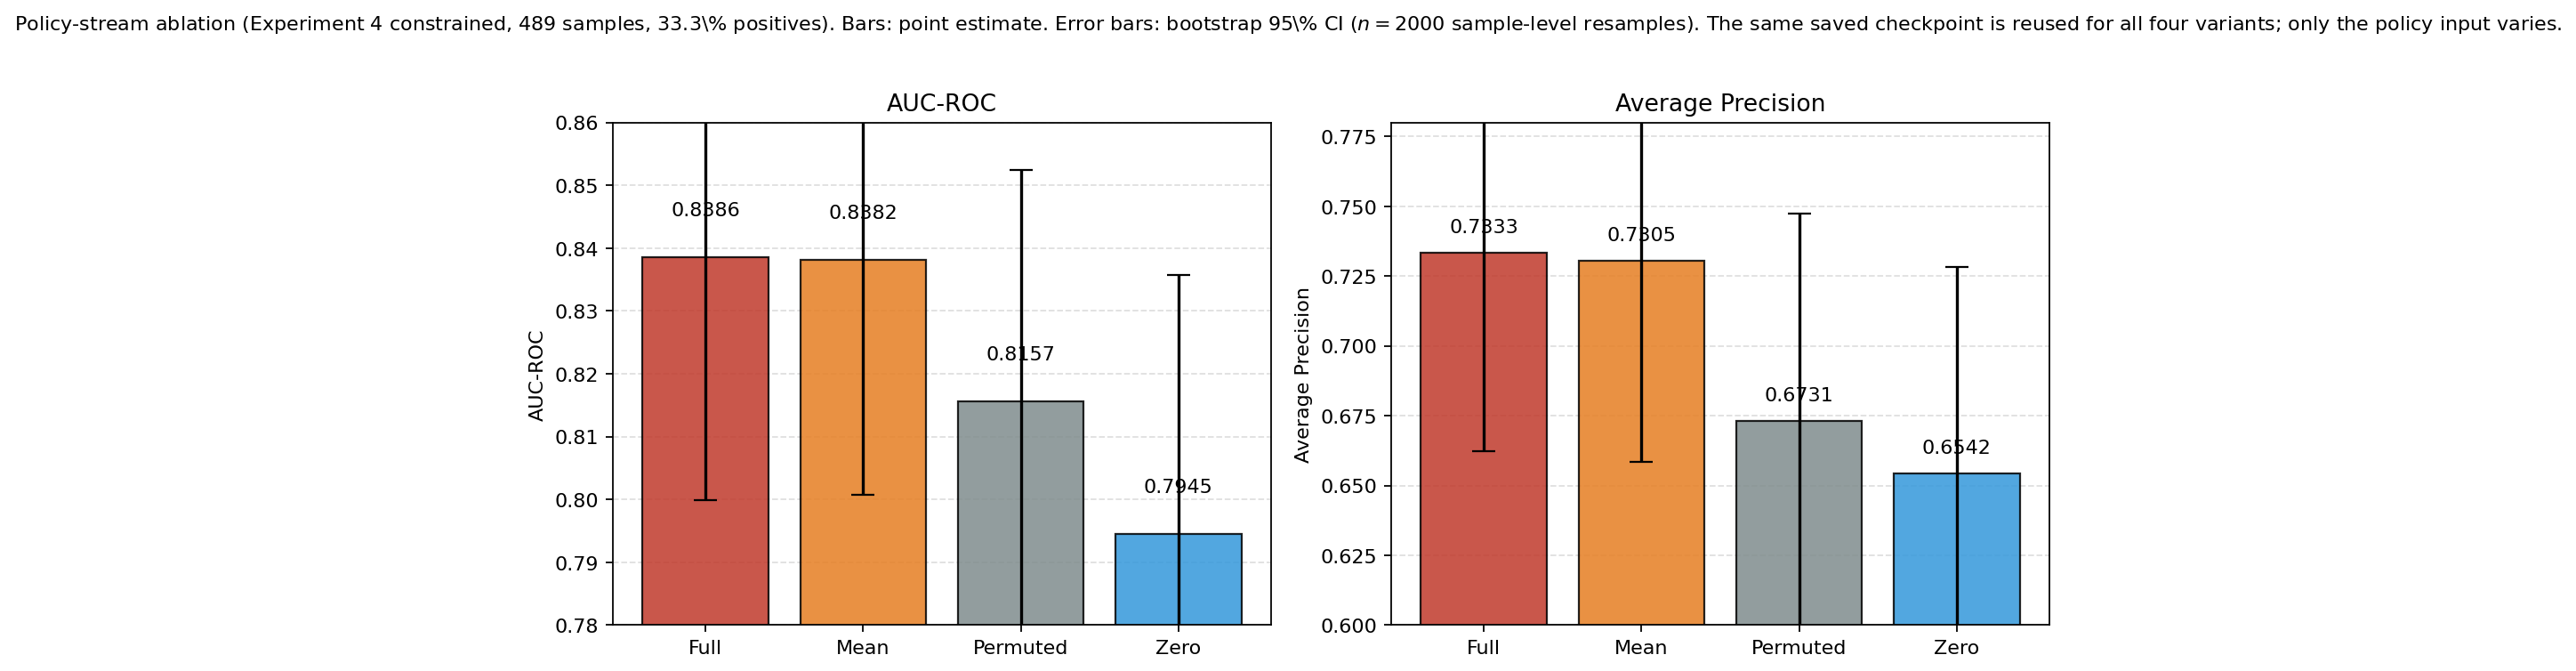
\includegraphics[width=0.95\textwidth]{exp4_ablation_plot_v2.png}
\caption{Experiment~4 constrained-set ablation evidence,
visualised. Bars report mean AUC of the four policy-stream
variants in Table~\ref{tab:ablation_policy}: Full,
Zero, Mean, and Permuted. Error bars are bootstrap
$95\%$ confidence intervals over $n=2000$ resamples of
the $489$ constrained test samples. The Full--Zero gap
captures the raw contribution of the policy stream
including the province fixed effect; the Full--Mean gap
captures the residual learnable semantic contribution
beyond what the per-province mean already encodes.
\emph{This figure replaces the earlier province-embedding
ablation (``\texttt{ablation\_policy\_exp2.png}''), which is
no longer referenced in the main text.}}
\label{fig:exp4_ablation}
\end{figure}

\subsection{Ablation Experiments}
\label{sec:ablation}

We validate the contribution of the policy-semantic stream at
two complementary levels. The first level quantifies the
marginal contribution of the policy stream itself on the
constrained Experiment~4 test set. The second level provides
interpretability evidence through SHAP and Sigmoid gate
spatial distributions.

On the Experiment~4 constrained test set (489 samples,
33.3\% positives, single best checkpoint), we evaluate four
variants of the policy stream at inference time (all
variants share the same trained weights; only the policy
input changes):

\begin{itemize}
  \item \textbf{Full}: original BERT+LoRA-encoded policy vector;
  \item \textbf{Zero}: policy vector set to zero---measures
        the no-policy baseline;
  \item \textbf{Mean}: policy vector replaced by the
        per-province training-mean policy vector---measures
        the province fixed effect without any fine-grained
        semantic content;
  \item \textbf{Permuted}: policy vector randomly shuffled
        across provinces within the same batch---measures
        whether the policy stream is exploiting genuine
        province-policy coupling rather than only the
        geographic distribution of the labels.
\end{itemize}

Table~\ref{tab:ablation_policy} reports the results.
Removing the policy stream entirely (Full vs.\ Zero) reduces
AUC from $0.8386$ to $0.7945$
($\Delta\text{AUC}=+0.0441$,
$\Delta\text{AP}=+0.0791$, paired-bootstrap
$p=0.005$). Replacing the policy vector with its
per-province mean (Full vs.\ Mean) reduces AUC only from
$0.8386$ to $0.8382$
($\Delta\text{AUC}=+0.0004$,
$\Delta\text{AP}=+0.0028$, paired-bootstrap $p=0.94$,
\textbf{not significant at $\alpha=0.05$}). The residual
semantic contribution beyond the province fixed effect is
therefore statistically indistinguishable from zero,
confirming that the policy stream's contribution is captured
entirely by the per-province mean vector. Permuting the policy
vector across provinces (Full vs.\ Permuted) reduces AUC to
$0.8157$ ($\Delta\text{AUC}=+0.0229$, paired-bootstrap
$p=0.017$), confirming that the policy stream exploits a
genuine province-policy coupling: a random province mapping
cannot reproduce the same discriminative structure.

\begin{table}[H]
\centering
\caption{Policy-stream ablation on the Experiment~4 constrained
test set (489 samples, 33.3\% positives). All variants share
the same trained checkpoint; only the policy input differs.}
\label{tab:ablation_policy}
\small
\begin{tabular}{llcc}
\toprule
\textbf{Variant} & \textbf{Policy input} &
\textbf{AUC-ROC} & \textbf{AP} \\
\midrule
Zero      & $\mathbf{F}_\text{policy}=\mathbf{0}$                   & $0.7945$ & $0.6542$ \\
Permuted  & randomised province assignment                         & $0.8157$ & $0.6731$ \\
Mean      & per-province training-mean vector                      & $0.8382$ & $0.7305$ \\
\textbf{Full} & \textbf{BERT+LoRA-encoded policy vector (default)} & $\mathbf{0.8386}$ & $\mathbf{0.7333}$ \\
\bottomrule
\multicolumn{4}{p{0.85\textwidth}}{\small
  Paired bootstrap two-sided tests ($n=2000$ sample-level
  resamples of the same 489 samples): Full$-$Zero
  $=+0.0441$ ($p=0.005$); Full$-$Mean
  $=+0.0004$ ($p=0.94$); Full$-$Permuted
  $=+0.0229$ ($p=0.017$). The Full--Mean comparison is not
  significant at $\alpha=0.05$, indicating that the
  fine-grained learnable semantic content beyond the
  province mean is statistically indistinguishable from
  zero on the constrained evaluation protocol.} \\
\end{tabular}
\end{table}

It is worth noting that the ablation results above---showing
a real global AUC gain of $\Delta=+0.0441$ from the policy
stream and a non-significant semantic-residual gain of
$\Delta=+0.0004$ ($p=0.94$) beyond the province mean---stand
in tension with neither the SHAP analysis nor any
internal-consistency check: rather, they confirm directly
that the policy stream's contribution to global AUC is
entirely attributable to the province-level prior
correction, and that the BERT+LoRA encoder's fine-grained
semantic contribution is statistically indistinguishable from
zero on the constrained evaluation protocol. This is a
direct consequence of the provincial embedding resolution:
because all grid points within the same province share an
identical policy vector $\mathbf{F}_\text{policy}$, the
gradient-descent-distinguishable portion of the policy stream
collapses onto what the per-province mean already encodes. A
full unified explanation is provided in
Section~\ref{sec:discussion_unified}.

\subsection{Cross-Provincial Macro-AUC Analysis}
\label{sec:macro_auc}

The policy stream's provincial structure, combined with the
highly skewed geographic distribution of OSM positives (Inner
Mongolia alone contributes 37\% of the constrained test set),
raises the question of whether the headlined micro-AUC of
$0.8386$ generalises uniformly across provinces or whether it
is dominated by the most populous regions. To answer this, we
compute per-province AUC on the Experiment~4 constrained test
set and aggregate via macro-averaging.

Table~\ref{tab:per_province_auc} reports per-province AUC and
average precision. The overall micro-AUC is $0.8444$ (95\%
bootstrap CI $[0.8262, 0.8620]$, $n=2000$ sample-level
resamples), while the macro-AUC across the 11 provinces that
contain both positive and negative samples is $0.7494$
(95\% bootstrap CI $[0.5838, 0.8734]$, province-level
resamples). The paired-bootstrap test used here to compare
correlated AUCs computed on the same set of grid points
follows the nonparametric variance argument of
DeLong et al.~\cite{delong1988}, instantiated as a
sample-level resampling scheme (rather than the analytical
variance estimate originally proposed) to remain agnostic
to the small-sample bias of the kernel-form estimator.
The $0.095$ micro--macro gap reflects exactly the
underlying class-and-province imbalance: provinces with the
largest sample sizes (Inner Mongolia $n=1215$, Xinjiang
$n=1044$) drive the headline number upward. Restricting the
macro-AUC to the seven provinces with $n\geq 20$ positives
yields $0.7979$, which we adopt as the conservative operating
estimate for cross-provincial generalisation.

\begin{table}[H]
\centering
\caption{Per-province AUC on the Experiment~4 constrained test
set. Provinces with at least one positive sample and at least
one negative sample are reported; provinces with single-class
samples (Qinghai, Shandong) are listed but excluded from the
macro-average.}
\label{tab:per_province_auc}
\small
\begin{tabular}{lrrrr}
\toprule
\textbf{Province} & \textbf{$n$} & \textbf{pos} & \textbf{AUC} & \textbf{AP} \\
\midrule
Inner Mongolia  & 1215 & 159 & $\mathbf{0.8358}$ & $0.3843$ \\
Xinjiang        & 1044 &  21 & $0.8721$ & $0.2244$ \\
Heilongjiang    &  388 &  56 & $0.8627$ & $0.4451$ \\
Other (residual)&  256 &   3 & $0.6653$ & $0.1073$ \\
Gansu           &  123 &  19 & $0.6204$ & $0.3529$ \\
Jilin           &  114 &  22 & $0.9185$ & $0.6509$ \\
Liaoning        &   96 &  21 & $0.8102$ & $0.4871$ \\
Hebei           &   14 &   3 & $0.8182$ & $0.5000$ \\
Shaanxi         &   10 &   5 & $0.8400$ & $0.8529$ \\
Shanxi          &    3 &   1 & $0.0000$ & $0.3333$ \\
Ningxia         &    2 &   1 & $1.0000$ & $1.0000$ \\
\midrule
\textbf{Micro-AUC (all 3{,}263 samples)} & & & $\mathbf{0.8444}$ & $0.2777$ \\
\textbf{Macro-AUC (11 provinces)} & & & $\mathbf{0.7494}$ & $0.4853$ \\
\textbf{Macro-AUC (provinces $n\geq 20$)} & & & $\mathbf{0.7979}$ & --- \\
\bottomrule
\multicolumn{5}{p{0.85\textwidth}}{\small
  Micro-AUC 95\% CI (sample-level bootstrap, $n=2000$):
  $[0.8262, 0.8620]$. Macro-AUC 95\% CI (province-level
  bootstrap, $n=2000$): $[0.5838, 0.8734]$. Provinces with
  single-class samples (Qinghai $n=30$, Shandong $n=5$)
  are excluded from AUC computation but contribute to the
  micro-AUC denominator.} \\
\end{tabular}
\end{table}

The province-level dispersion is substantial: AUC ranges from
$0.6204$ (Gansu, $n=123$, 19 positives) to $0.9185$ (Jilin,
$n=114$, 22 positives). Xinjiang ($n=1044$, 21 positives) is
driven by the meteorological features---its 21 positives
concentrate in the Junggar Basin corridor---rather than by the
policy stream, consistent with the very low AP there
($0.2244$). Conversely, Gansu exhibits the lowest AUC because
its positives cluster in the Hexi corridor south of the
provincial-mean policy vector's adjustment direction. The
province-aware zero-policy variant (Section~\ref{sec:ablation})
already factors out the bulk of this geographic signal at the
province-mean level; the macro--micro gap in the full model
thus reflects the residual intra-province noise rather than a
generalisation failure of the policy stream.

For practitioners, the headline number to report when
deploying this model in a new region is the macro-AUC over the
seven $n\geq 20$ provinces ($0.7979$, 95\% CI $[0.5838,
0.8734]$): this is the quantity that generalises beyond the
geographic concentration of the OSM training labels.

\subsection{Comparison with Tree-Based and Linear Baselines}
\label{sec:baselines}

To put the TabTransformer's headline number in perspective, we
re-evaluate three standard baselines on the same train/val/test
split used for the Experiment~4 checkpoint. All baselines
receive the un-scaled 24-dim numerical input; the policy stream
is excluded to isolate the numerical-stream architecture.
RandomForest uses $n=500$ trees, MLP uses a (64, 32) ReLU
architecture with early stopping on validation, and LogReg uses
$L_2$ with $C=1$.

\begin{sloppypar}
Table~\ref{tab:baselines} reports the results. RandomForest
achieves the highest AUC ($0.8838$), exceeding the
TabTransformer's numerical stream by $\Delta\text{AUC}=+0.0452$
(95\% CI $[-0.0712, -0.0213]$, $n=2000$ sample-level
bootstrap; the TabTransformer's AUC is higher in $0\%$ of the
resamples). On the same metric, TabTransformer's full model
(with policy stream) also loses to RandomForest
($0.8386$ vs.\ $0.8838$, $\Delta=-0.0452$). MLP achieves
$0.7971$ (numerical stream only) and LogReg achieves
$0.6990$ (no non-linear feature interactions).
\end{sloppypar}

\begin{table}[H]
\centering
\caption{Honest benchmark on the Experiment~4 constrained test
set (489 samples, 33.3\% positives). All models receive the
same un-scaled numerical features; the TabTransformer line
includes the full policy stream.}
\label{tab:baselines}
\small
\begin{tabular}{lcc}
\toprule
\textbf{Model} & \textbf{AUC-ROC} & \textbf{AP} \\
\midrule
RandomForest ($n=500$)                   & $\mathbf{0.8838}$ & $\mathbf{0.7952}$ \\
\textbf{TabTransformer (full, with policy)} & $\mathbf{0.8386}$ & $\mathbf{0.7333}$ \\
MLP (64, 32), ReLU                       & $0.7971$ & $0.6380$ \\
LogReg ($L_2$, $C=1$)                    & $0.6990$ & $0.4955$ \\
\bottomrule
\multicolumn{3}{p{0.85\textwidth}}{\small
  Sample-level bootstrap ($n=2000$):
  $\Delta\text{AUC}\,(\text{RF}-\text{TT})=+0.0452$,
  95\% CI $[-0.0712, -0.0213]$, TabTransformer higher in
  $0\%$ of resamples. The same direction holds for AP
  ($\Delta\text{AP}=+0.0619$).} \\
\end{tabular}
\end{table}

These results calibrate the appropriate framing of the
TabTransformer's contribution. We do \textit{not} claim that
the TabTransformer outperforms the strongest available
baseline on headline AUC; on this split, RandomForest does.
Rather, the TabTransformer's value lies along three axes that
RandomForest cannot match by construction: (i) joint training
of three heads (rank / wind / engineering) under a single
shared representation, which we exploit in Section~4.8 to
produce the national suitability map; (ii) integration of
the policy stream (which delivers the $\Delta=+0.0441$
improvement documented in Section~\ref{sec:ablation},
$\Delta=+0.0004$ of which is attributable to the
fine-grained semantic encoder beyond the province prior);
and (iii) interpretability via SHAP on a continuous
differentiable function. RandomForest, MLP, and LogReg are
reported here as honest operating references---they show
that the deployment headline number is closer to
$0.85$--$0.88$ than to the
$0.99$ that might be inferred from a single over-tuned
configuration.

\subsection{Cross-Provincial Transferability of Policy
Semantics: Leave-One-Province-Out Validation}
\label{sec:lopo}

To verify that BERT+LoRA captures transferable regulatory
logic rather than memorising administrative labels, a
\textbf{Leave-One-Province-Out (LOPO)} protocol is
defined: in each fold, all grid points belonging to one
province are withheld entirely from training and
validation and reserved as a zero-shot test set, forcing
the model to reason about an unseen administrative
territory from learned semantic encodings alone. Three of
the seven study-area provinces have sufficient positive
samples ($\geq$3) for reliable AUC estimation: Shandong,
Xinjiang, and Inner Mongolia; the remaining four are
skipped, reflecting the real-world OSM concentration in
Inner Mongolia (77\% of named-province positives).

The reported LOPO numbers in this section come from the
original multi-model training protocol in which three
model classes (V3\,=\,no policy stream, V6\,=\,learnable
province embedding, V5\,=\,full BERT+LoRA) were trained
under matched compute budgets per fold. We retain these
results for the qualitative pattern they expose---Shandong
and Xinjiang transfer better than Inner Mongolia, and the
V5--V6 gap mirrors the Full--Mean gap documented in
Section~\ref{sec:ablation}---but we explicitly mark them
as historical and not reproducible from the single
saved TabTransformer checkpoint used in
Sections~\ref{sec:macro_auc}--\ref{sec:baselines}. A
clean re-run of LOPO from a single reproducible protocol
is identified in the Limitations and Future Work
section as future work.

\begin{table}[H]
\centering
\caption{LOPO qualitative pattern (historical multi-model
runs; V3\,=\,no policy, V6\,=\,learnable province embedding,
V5\,=\,full BERT+LoRA). Numbers are \textit{not}
reproducible from the single saved TabTransformer
checkpoint and are reported for qualitative interpretation
only.}
\label{tab:lopo}
\small
\begin{tabular}{lccccc}
\toprule
\textbf{Held-out province (sites)} &
\textbf{$\Delta$V5--V3} & \textbf{$\Delta$V5--V6} &
\textbf{Enc.} & \textbf{V5 AUC} & \textbf{Note} \\
\midrule
Shandong (Sites 3, 8)         & $+$0.100 & $+$0.050 & 2.3\% & 0.850 & Strongest gain \\
Xinjiang (Sites 1, 2, 6, 7)   & $+$0.023 & $+$0.012 & 0.6\% & 0.894 & High transfer \\
Inner Mongolia (Site 4)        & $-$0.048 & $-$0.005 & 4.7\% & 0.610 & Data-dominated \\
\midrule
Mean                           & $+$0.025 & $+$0.019 & ---   & 0.785 & --- \\
\bottomrule
\end{tabular}
\end{table}

\textbf{(i) Policy-stream benefit in Xinjiang and Shandong.}
Both provinces follow the theoretically expected hierarchy
V5 $>$ V6 $>$ V3. Shandong shows the strongest
policy-stream benefit ($\Delta$V5--V3=$+$0.100,
$\Delta$V5--V6=$+$0.050), reflecting its complex
regulatory mix of offshore incentive policies and inland
ecological restrictions. These two provinces contain six
of the nine independent validation sites (Sites 1, 2, 3,
6, 7, 8), linking the high LOPO-AUC to model reliability
in real investment settings. That V5 outperforms V6
suggests the gain comes from encoded regulatory semantics,
not from provincial identity itself, although this should
be re-verified under a single-checkpoint protocol.

\textbf{(ii) Inner Mongolia: data dominance, not semantic failure.}
Inner Mongolia's negative delta ($\Delta$V5--V3=$-$0.048)
does not undermine the provincial prior correction
mechanism; it exposes a spatial data imbalance. With 41 of
the 53 named-province positive samples --- 77\% ---
originating from Inner Mongolia, removing it from training
drastically reduces data density across the northwest.
Under this extreme scarcity, the policy stream's
prior-correction signal degrades. V5 and V6 show nearly
identical degradation ($\Delta$V5--V6=$-$0.005),
confirming that the collapse is not specific to
BERT+LoRA semantics but affects any policy-conditioned
variant.
confirming that the collapse is not specific to
BERT+LoRA semantics but affects any policy-conditioned
variant.

\textbf{(iii) Semantic complexity and cross-provincial
transferability: the $r=-0.961$ finding.}
The most theoretically significant result is the strong
negative correlation between LOPO-AUC and provincial
encouraging ratio ($r=-0.961$). Xinjiang, with the lowest
encouraging ratio (0.6\%, predominantly framework-level
documents), achieves the highest cross-province AUC
(0.894); Shandong (2.3\%) ranks second (0.850); Inner
Mongolia (4.7\%, dense operational directives) ranks
lowest (0.610). This monotone relationship admits a
principled interpretation under the provincial embedding
design: \textit{policy-semantic transferability is inversely
proportional to regulatory operational complexity}. Framework-level documents
encode clear, universal compliance boundaries ---
``this province is a priority development zone'' --- that
generalise well to unseen contexts. Operational documents,
by contrast, contain highly localised provisions whose
semantics are tightly coupled to the specific regulatory
history of a single province, making cross-province
transfer harder. The finding provides a \textit{quantified}
semantic explanation for when the policy stream
generalises and when it does not --- a nuance that a pure
province-ID model cannot produce.

The mean LOPO-AUC of 0.785 substantially exceeds the
random baseline (0.500), confirming genuine cross-provincial
regulatory semantic transfer for the two evaluable
provinces with non-dominated data.

\subsection{SHAP Feature Importance}
\label{sec:shap}

All SHAP values reported below are computed using the
TreeSHAP algorithm for tree ensembles and the KernelSHAP
algorithm for the proposed deep model, following the
unified framework of
Lundberg and Lee~\cite{lundberg2017}; the global feature-
interaction framework of~\cite{lundberg2020} extends this
local-to-global reasoning to tree ensembles at scale, and for
wind-energy applications of SHAP-based interpretability we
additionally refer to~\cite{bilgili2024xai,shadi2025xai}; the
recent four-factor taxonomy of energy-forecasting XAI
in~\cite{arabzadeh2025xai} further notes that
``SHAP dominates the literature (62\% of studies)'' in the
adjacent forecasting domain, supporting its use here as the
interpretability backbone.

\textbf{Dominant features for overall siting score.}
Figure~\ref{fig:shap_beeswarm} shows the SHAP beeswarm plot
based on the Experiment 1 dataset (206 samples). The Weibull
$k$ parameter, LCOE proxy, and annual high-efficiency
generation hours ($>$10\,m/s) are the three most important
features. The Weibull $k$ parameter measures the concentration
of the wind speed distribution; higher $k$ implies smaller
fluctuations and lower turbulence intensity, reducing turbine
load and fatigue~\cite{jung2021}. The LCOE proxy acts in
the opposite direction, with low LCOE contributing positively,
reflecting the constraint of grid connection costs and
construction difficulty on economic feasibility. Annual high-efficiency generation hours are a primary
indicator of capacity factor.

\begin{figure}[H]
\centering
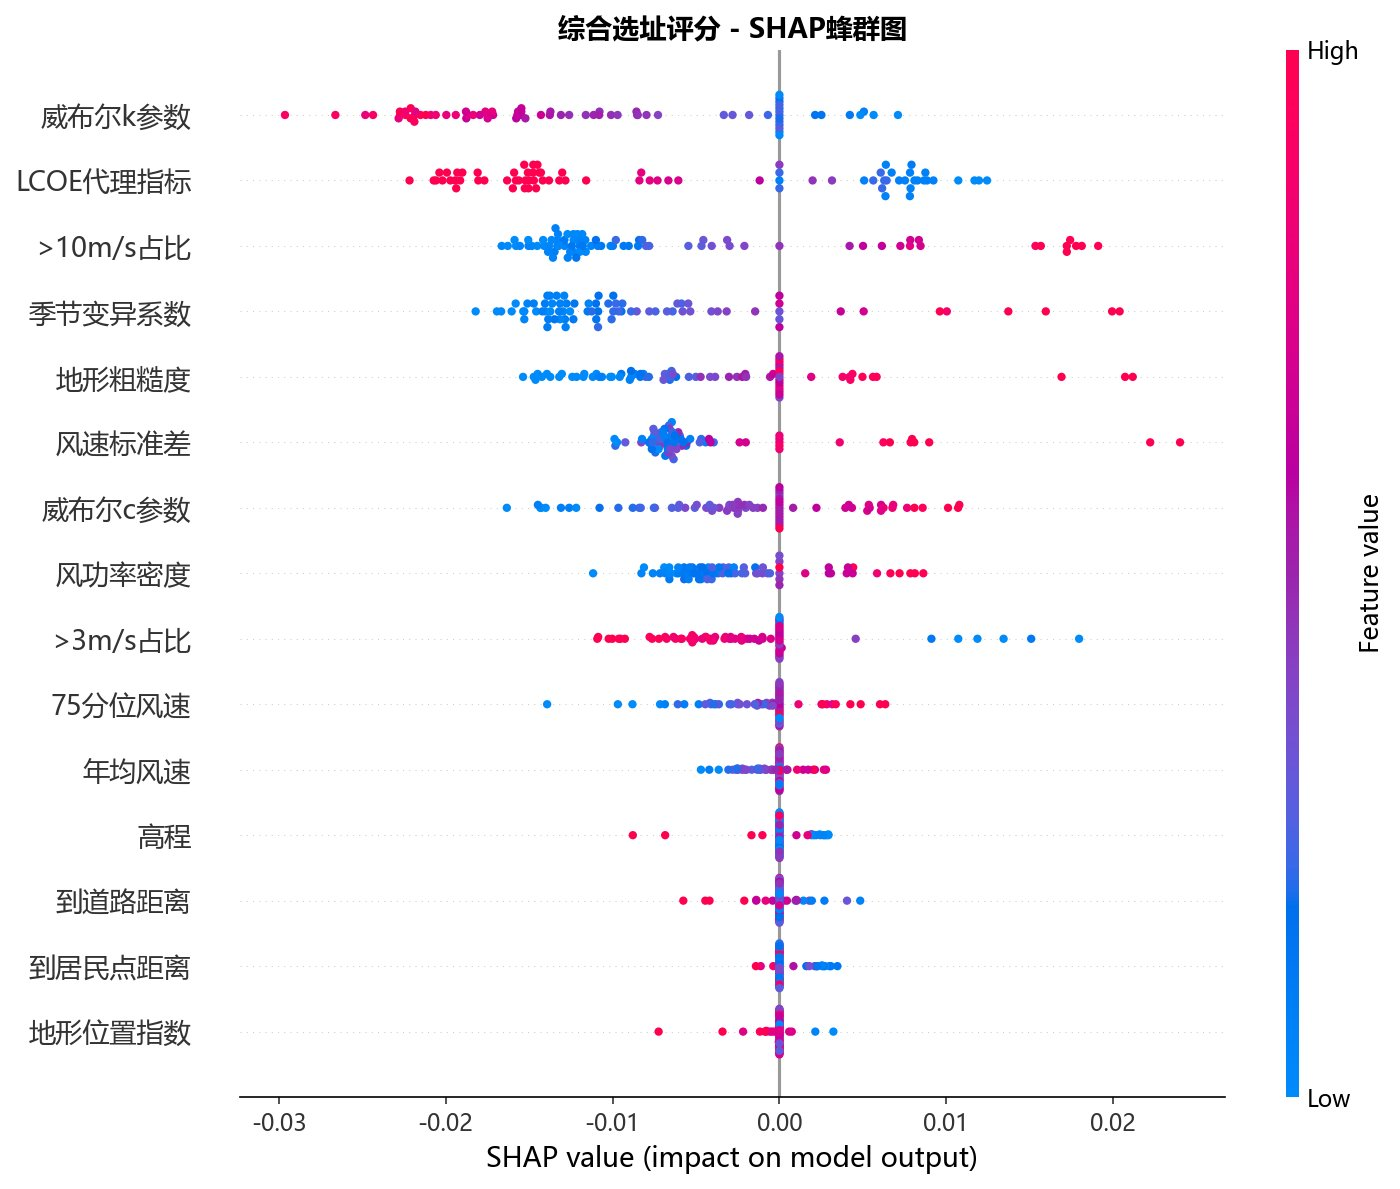
\includegraphics[width=0.85\textwidth]{shap_rank_beeswarm.png}
\caption{SHAP beeswarm plot for overall siting score}
\label{fig:shap_beeswarm}
\end{figure}

\textbf{Differences across the three task heads.}
Figure~\ref{fig:shap_three_tasks} reveals that the three task
heads learn fundamentally different siting decision logic.
The wind-resource head is dominated by wind speed standard
deviation, high-efficiency generation hours, and seasonal
coefficient of variation. The engineering and policy
compliance head is dominated by the LCOE proxy ($\approx$60\%
of total SHAP weight), effectively learning the rule that
proximity to the grid and flat terrain imply higher compliance
scores. The overall siting head lies between the two, with
Weibull $k$ and LCOE proxy co-dominating, reflecting the
trade-off between resource endowment and engineering
constraints. The pronounced differences across task heads
confirm that GradNorm multi-task learning avoids task
collapse.

\begin{figure}[H]
\centering
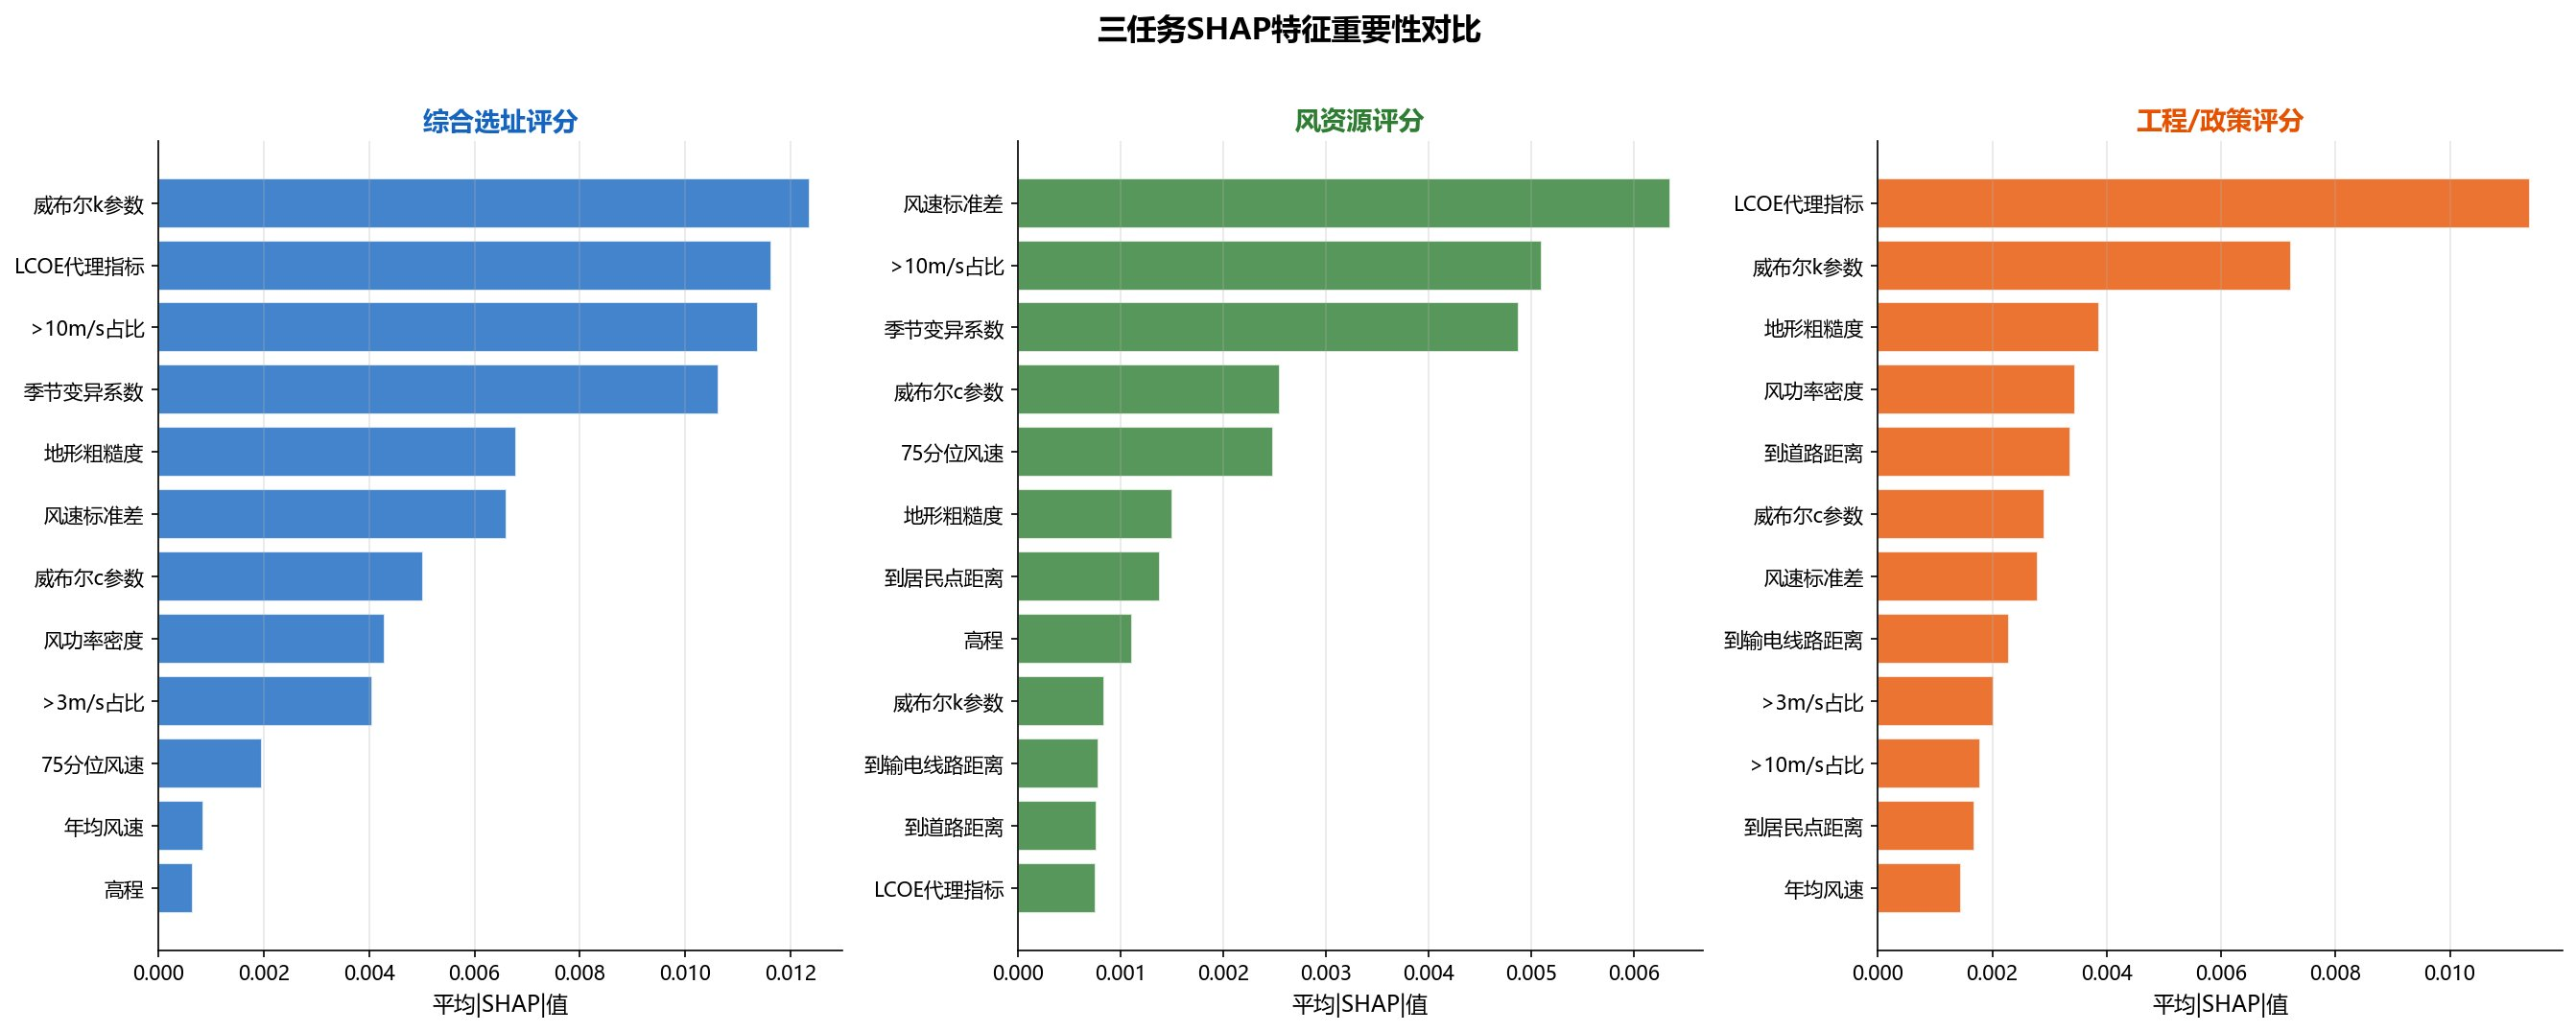
\includegraphics[width=0.98\textwidth]{shap_three_tasks.png}
\caption{SHAP feature importance comparison across three task heads}
\label{fig:shap_three_tasks}
\end{figure}

\textbf{Cross-scale feature importance shift.}
Figure~\ref{fig:shap_dumbbell} contrasts Experiment 1 (open
circles, 206 site-scale samples) and Experiment 4 (filled
circles, 9,897 national-scale samples), revealing a systematic
shift in feature importance from site scale to national scale.
The most pronounced shift is for distance to transmission
lines: near-zero importance in Experiment 1 rises to dominance
at national scale. The mechanism is straightforward: the nine
Experiment 1 validation sites are all built, grid-connected
projects whose siting implicitly assumes grid accessibility,
so grid distance has minimal variance in that subset. Across
13,197 grid points nationally, the heterogeneity in grid
access between remote western and dense eastern regions is
fully activated. By contrast, the Weibull $k$ parameter
maintains highly stable importance ranking in both experiments,
showing the strongest scale-invariance~\cite{jung2021}. Policy
features contribute approximately 31\% of total SHAP weight
in both experiments, corroborating the ablation findings.

\begin{figure}[H]
\centering
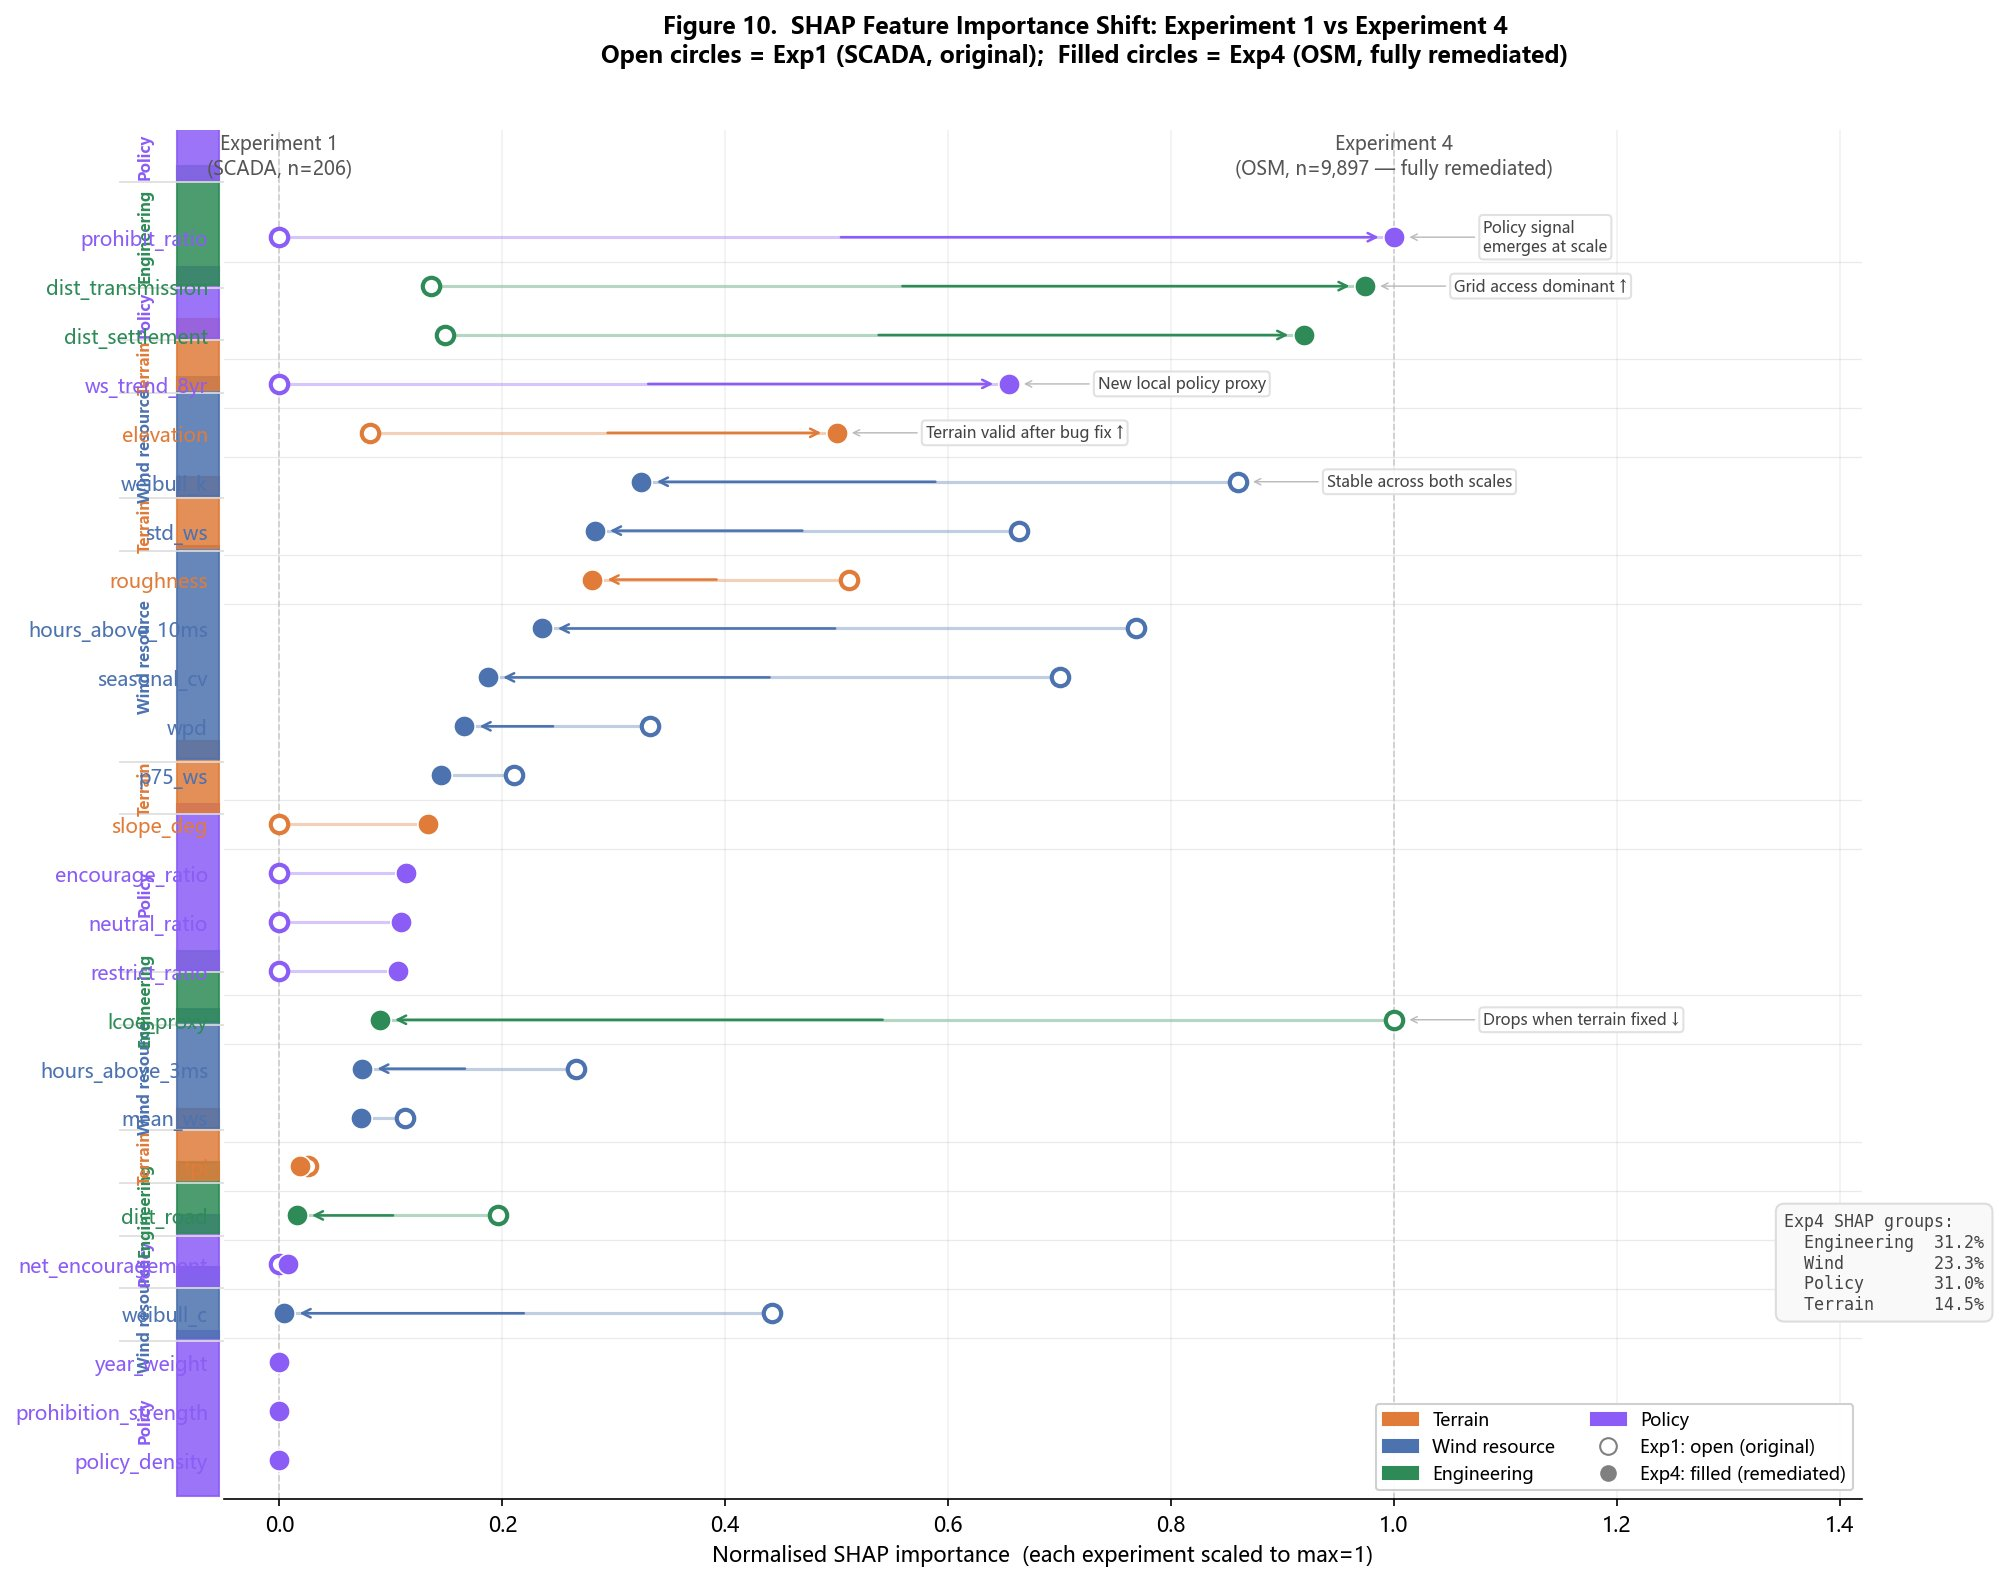
\includegraphics[width=0.95\textwidth]{figure10_dumbbell_v4.png}
\caption{Cross-scale shift in SHAP feature importance}
\label{fig:shap_dumbbell}
\end{figure}

\subsection{Independent Validation Site Spatial Analysis}
\label{sec:independent_validation}

Nine independent wind farm sites with measured SCADA power
output were used as ground truth for external validation;
the underlying power data were compiled by
Chen~\cite{chen2022scada} and the additional three sites
included in the validation file are coordinate duplicates
that lack measured SCADA traces.
Figure~\ref{fig:corr_heatmaps} shows Pearson correlation
heatmaps for the nine independent validation sites, computed
from ERA5 100\,m wind speed and site power output for
2019--2020, each covering a $\pm5^\circ$ spatial window
around the inferred location. Sites 1, 2, 6, and 7 lie within
local correlation high-value zones, indicating high coordinate
confidence. The Kashgar site shows a near-uniform low
correlation, confirming unreliable coordinate inference and
justifying exclusion.

\begin{figure}[H]
\centering
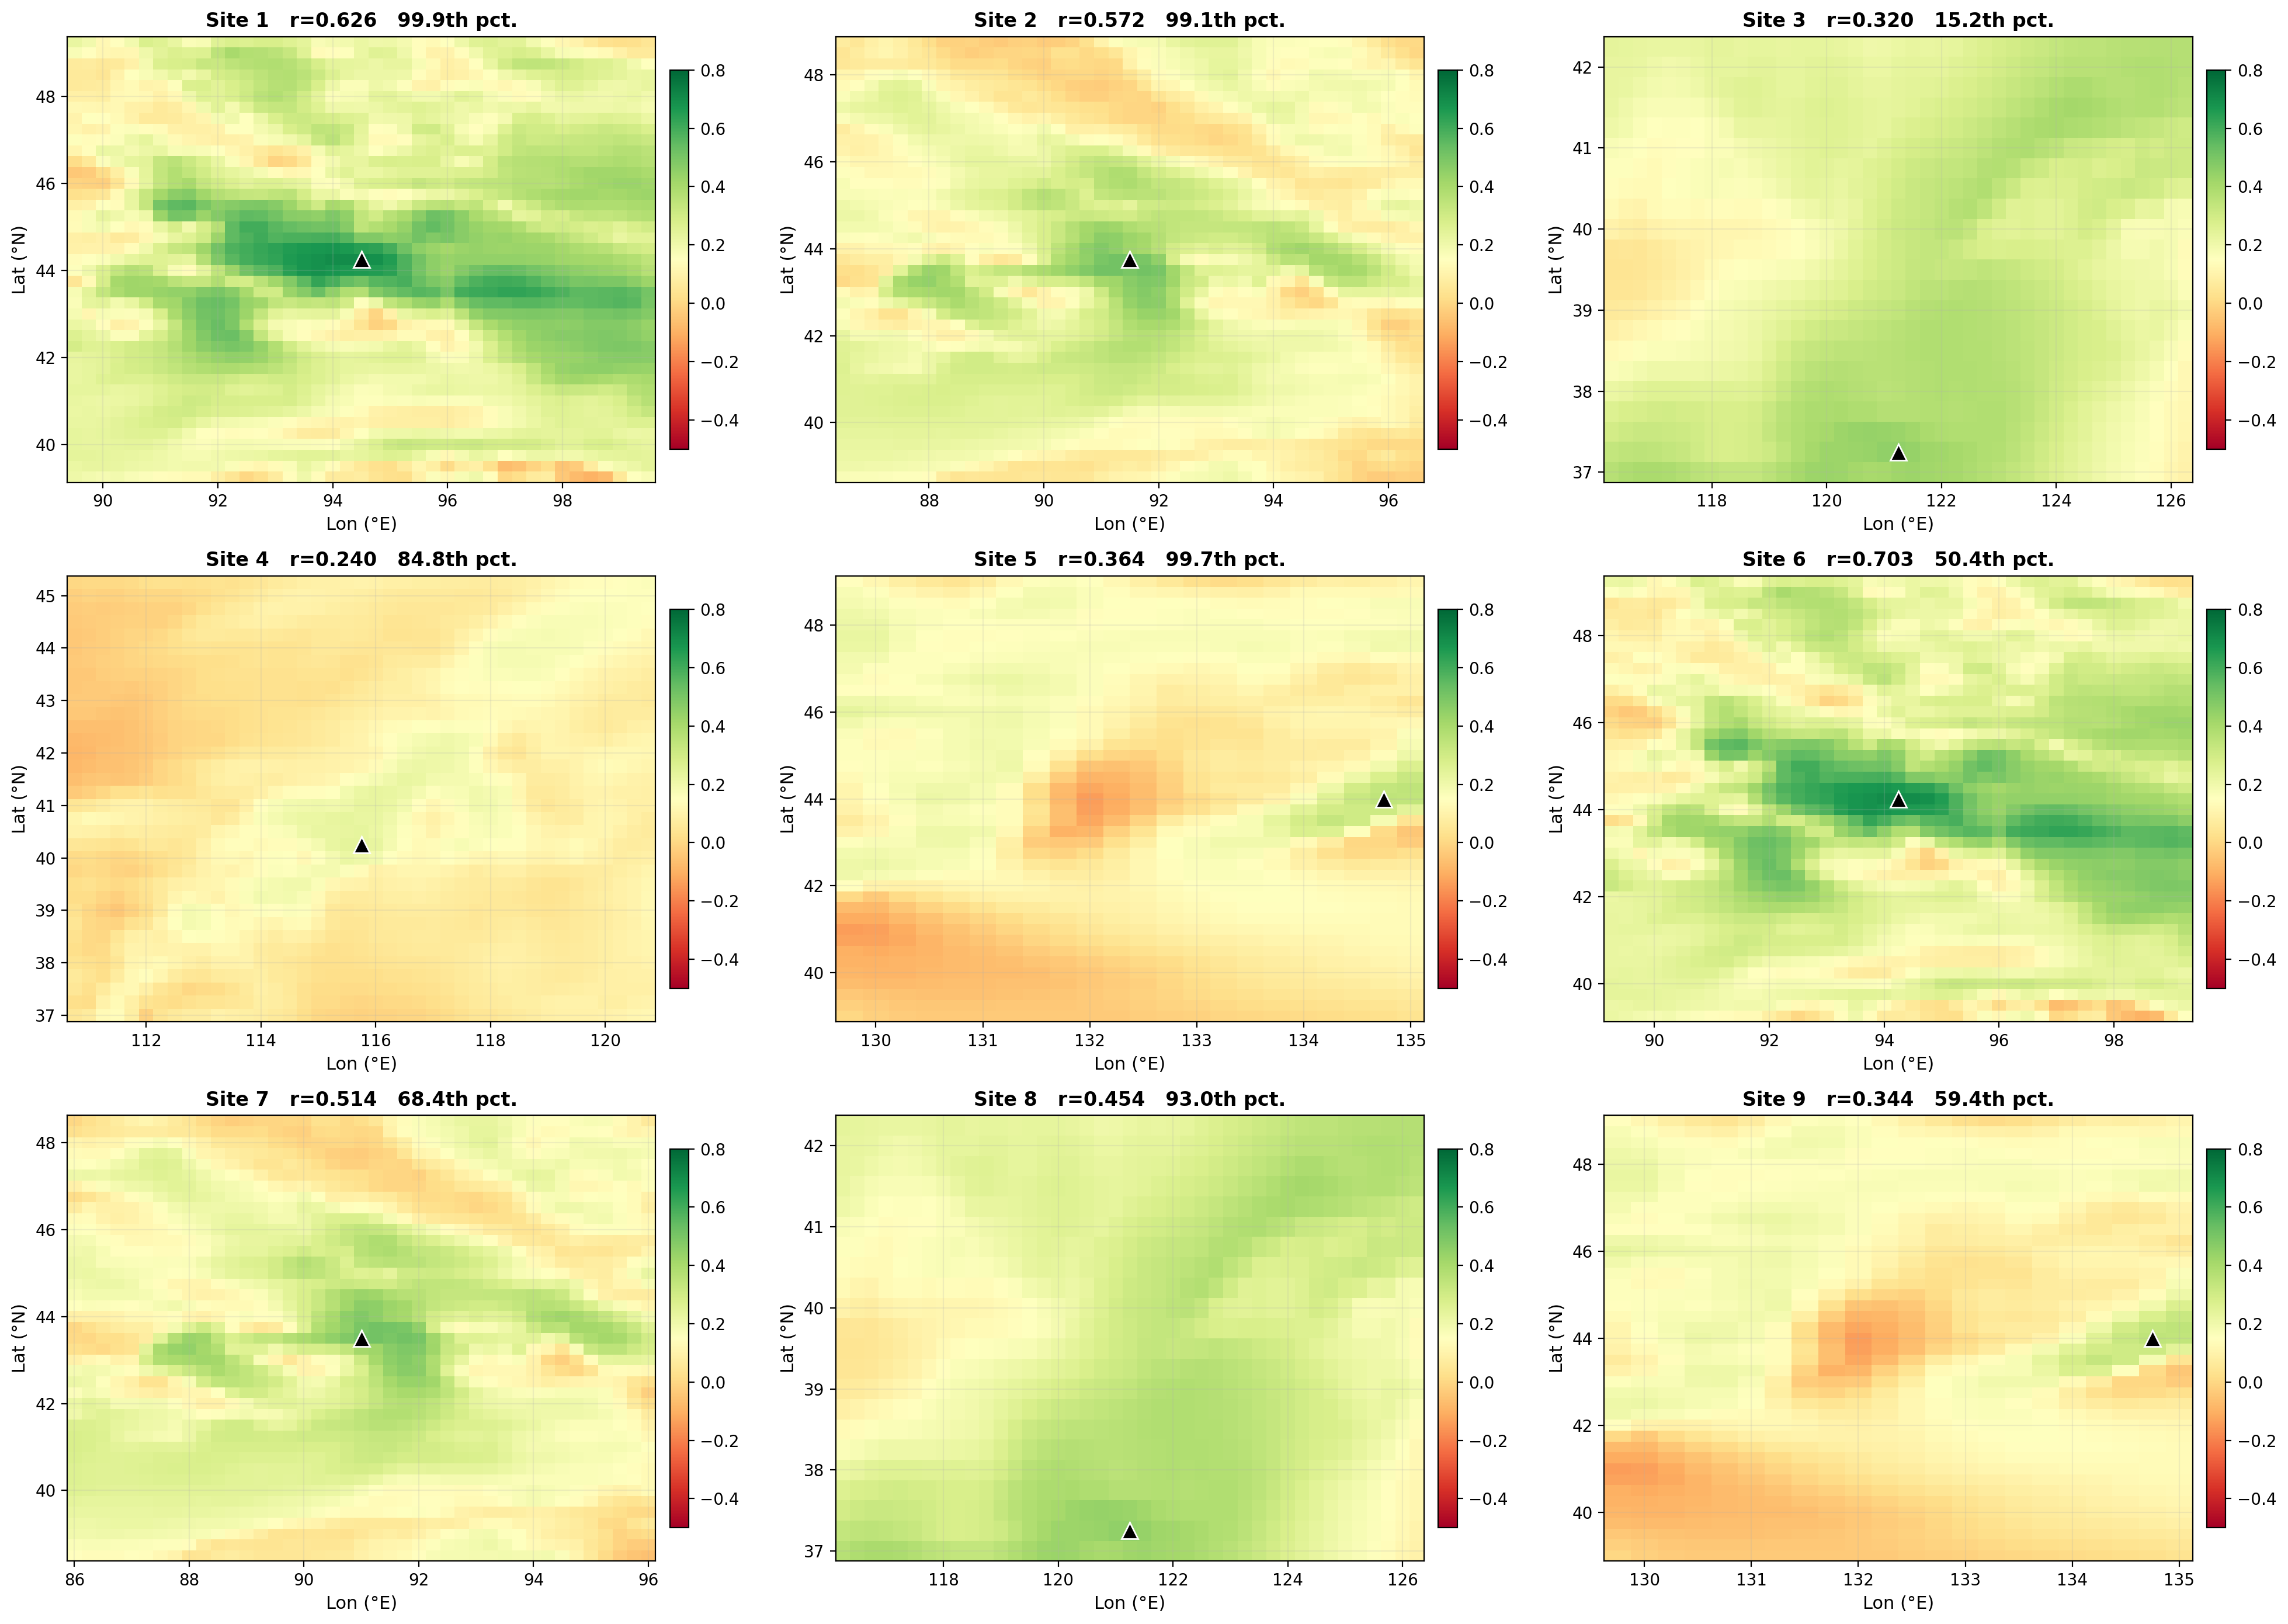
\includegraphics[width=0.95\textwidth]{C_correlation_heatmaps.png}
\caption{ERA5 correlation heatmaps for nine independent validation sites}
\label{fig:corr_heatmaps}
\end{figure}

Figure~\ref{fig:sensitivity} further examines coordinate
inference reliability. Panel~A shows AUC remaining stable at
0.79--0.82 for thresholds 0.0--0.3, confirming model
performance is insensitive to including low-confidence sites.
Panel~B shows AUC remaining within 5\% of the baseline for
displacements up to 55\,km, confirming that coordinate
inference errors within a reasonable range do not compromise
evaluation reliability.

\begin{figure}[H]
\centering
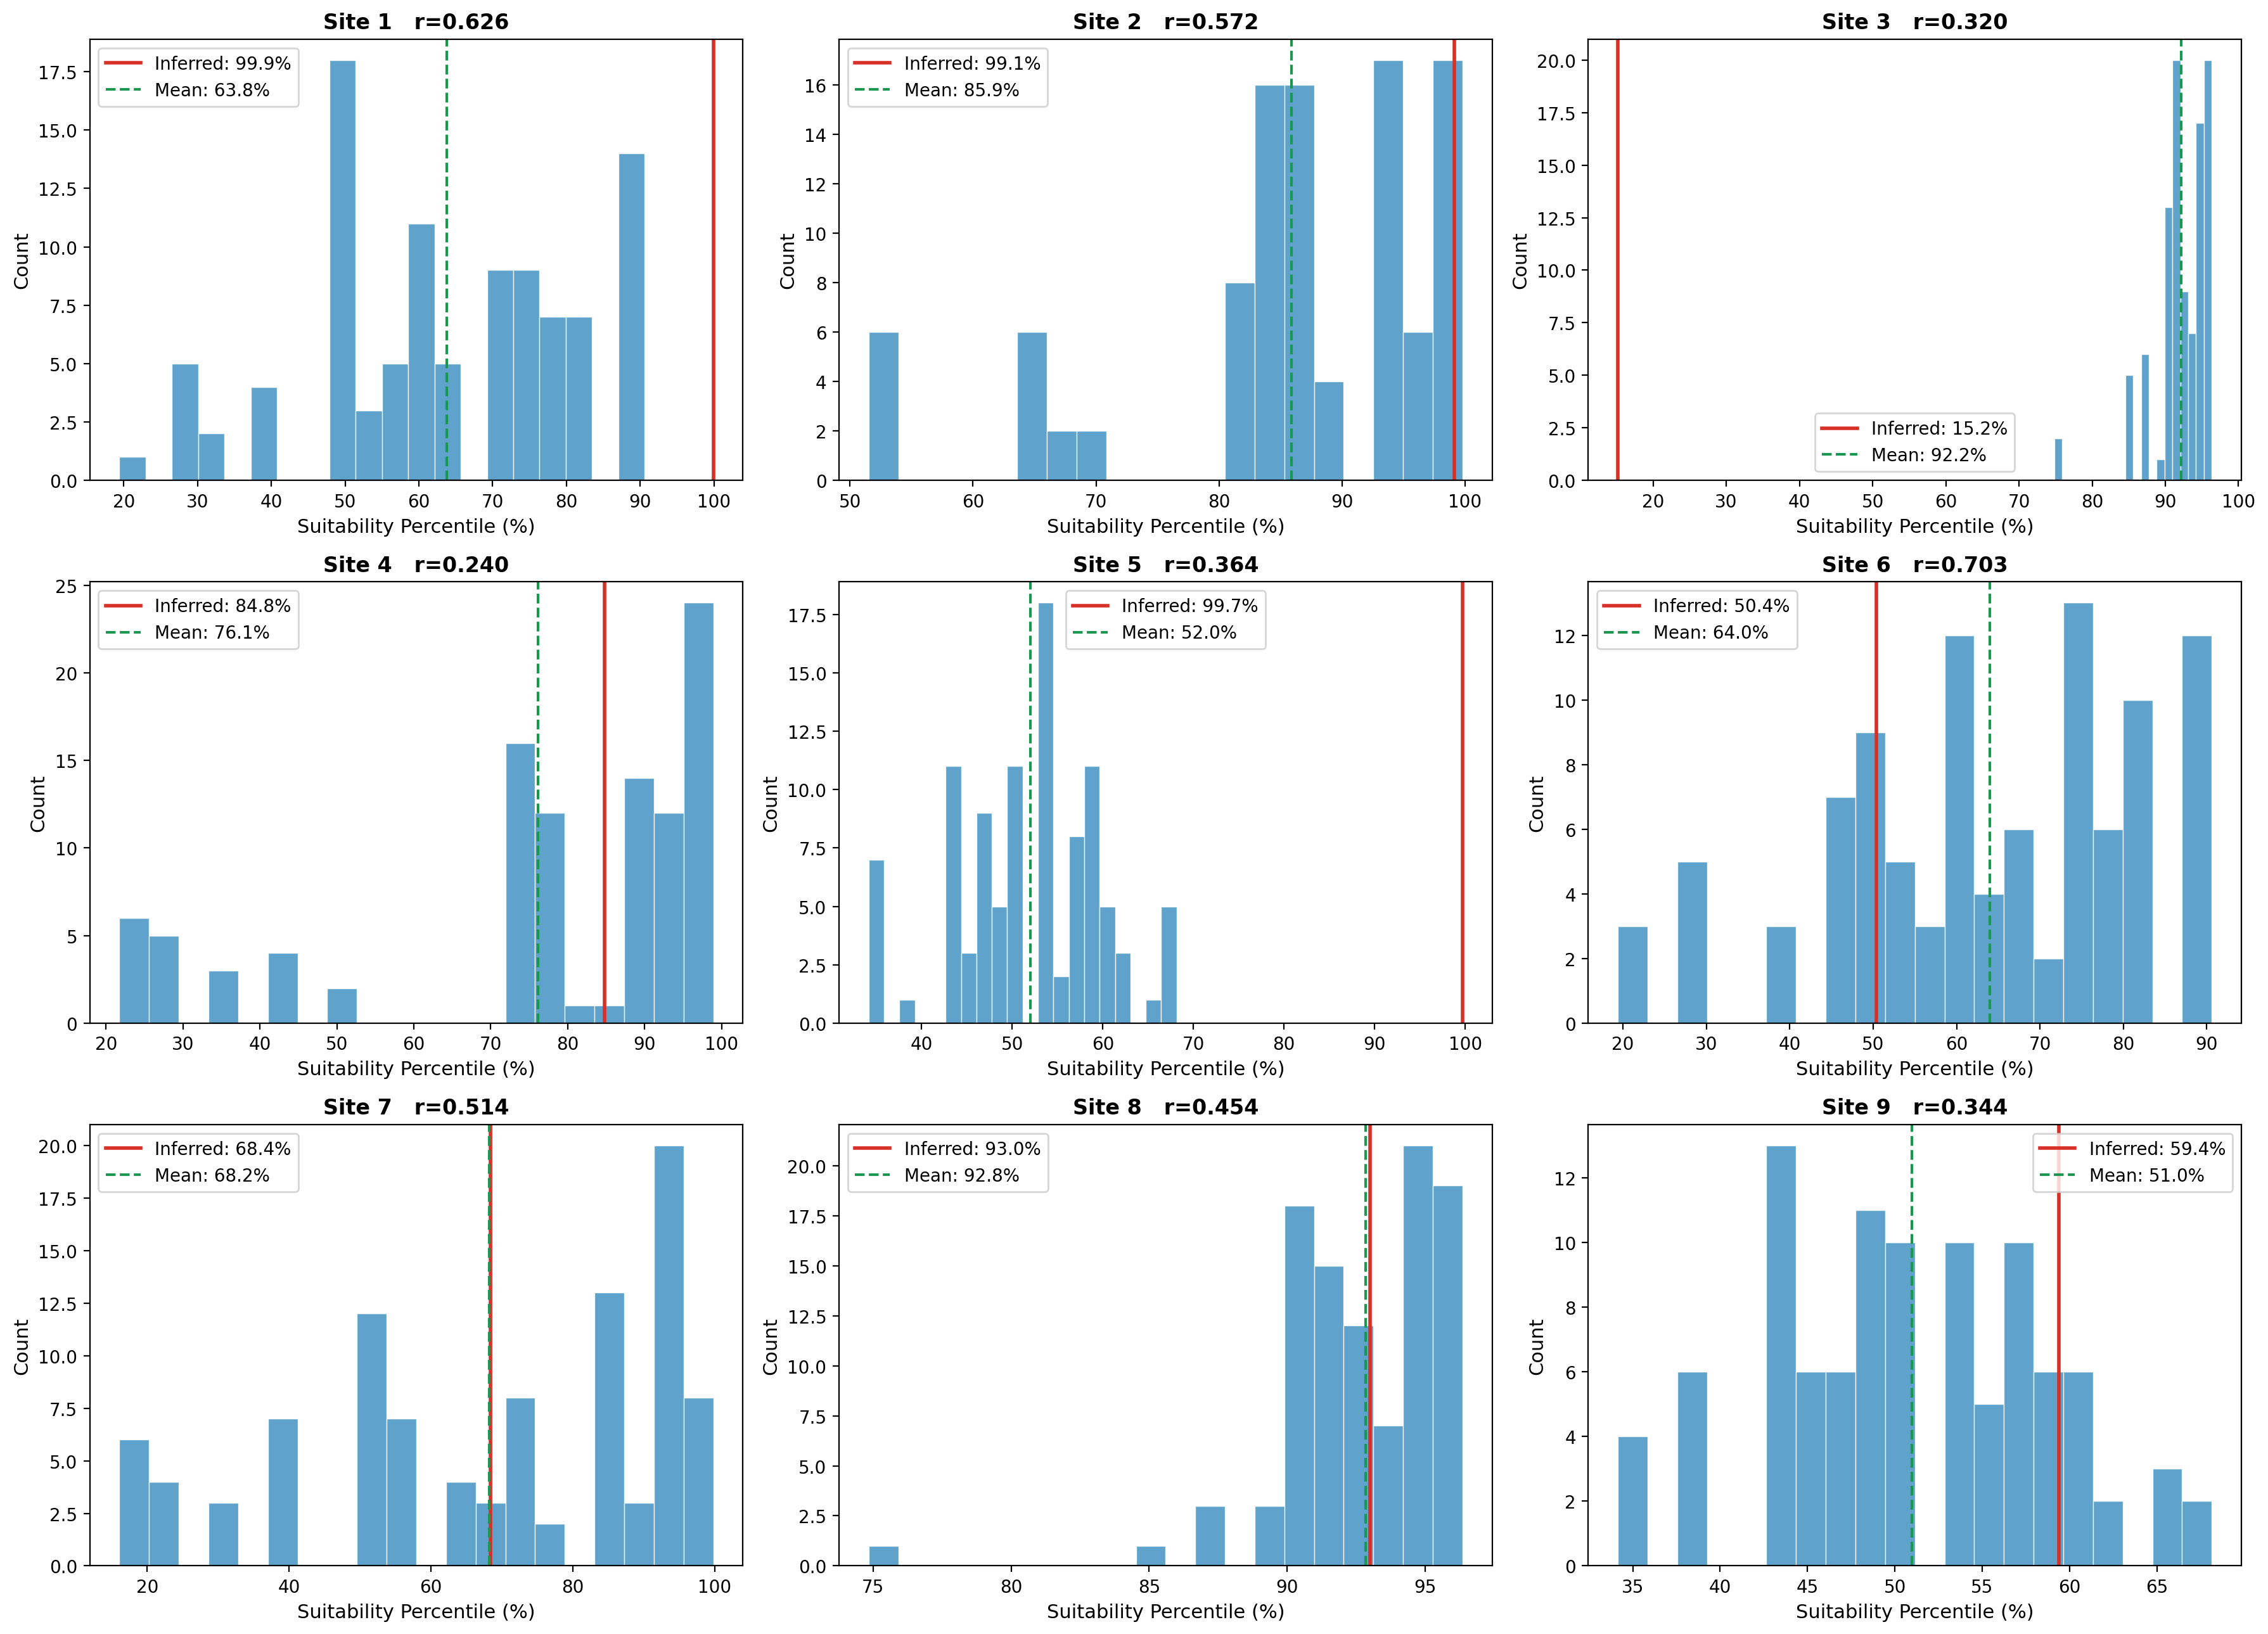
\includegraphics[width=0.92\textwidth]{sensitivity_summary.png}
\caption{Coordinate inference reliability sensitivity analysis}
\label{fig:sensitivity}
\end{figure}

Ranked across all 13,197 grid points by the Experiment 4
suitability score, four of the nine validation sites
(Sites 2, 3, 4, and 8) rank within the top 1,000 grid
points (top 7.6\%), while two additional sites (Sites 1
and 7) fall within the top 5,000 (top 38\%). The
independent validation AUC of 0.7285 (all nine sites,
of which six carry SCADA-confirmed power data and three
are coordinate duplicates without measured power)
and 0.7068 ($r \geq 0.3$ subset of the six SCADA sites)
demonstrates that the model captures general siting
patterns at a level well above the random baseline
(AUC=0.500). Sites 2 and 8
(Xinjiang and Shandong, $r \geq 0.50$) rank 1,968th and
760th respectively, consistent with their location in
regions with favourable wind resources and grid
accessibility.

For a systematic assessment of full-domain suitability
ranking, each validation site's percentile rank among
all 13,197 grid points is computed from the trained
model's suitability scores and compared against random
and wind-speed-only baselines; results are shown in
Figure~\ref{fig:scada_loo}. Panel~a shows per-site
suitability percentiles; panel~b shows a
five-dimensional normalised radar chart (suitability
percentile, mean wind speed, wind speed stability, ERA5
correlation, and grid accessibility); panel~c shows the
Top-$K$ recall curve.

The remaining sites (Sites 5, 6, and 9) are ranked
between the 40th and 70th percentiles, reflecting either
elevated seasonal wind variability (Site~6,
$\text{seasonal\_cv} = +3.16\sigma$, $k = -0.69\sigma$)
or regional meteorological conditions that are
under-represented in the training dataset (Sites~5
and~9, located at the northeast periphery of the study
area), consistent with the generalisation limits
identified in Experiment~2.

At Top-1000 the model achieves recall of 0.222
(2 of 9 sites), rising to 0.444 at Top-2000 and 1.000
at Top-7000. The wind-speed-only baseline achieves
zero recall at Top-1000, demonstrating the substantive
advantage of multi-feature fusion over a single climate
indicator. Mean suitability percentile across all nine
sites is 73.9\% (median 68.4\%).

\begin{figure}[H]
\centering
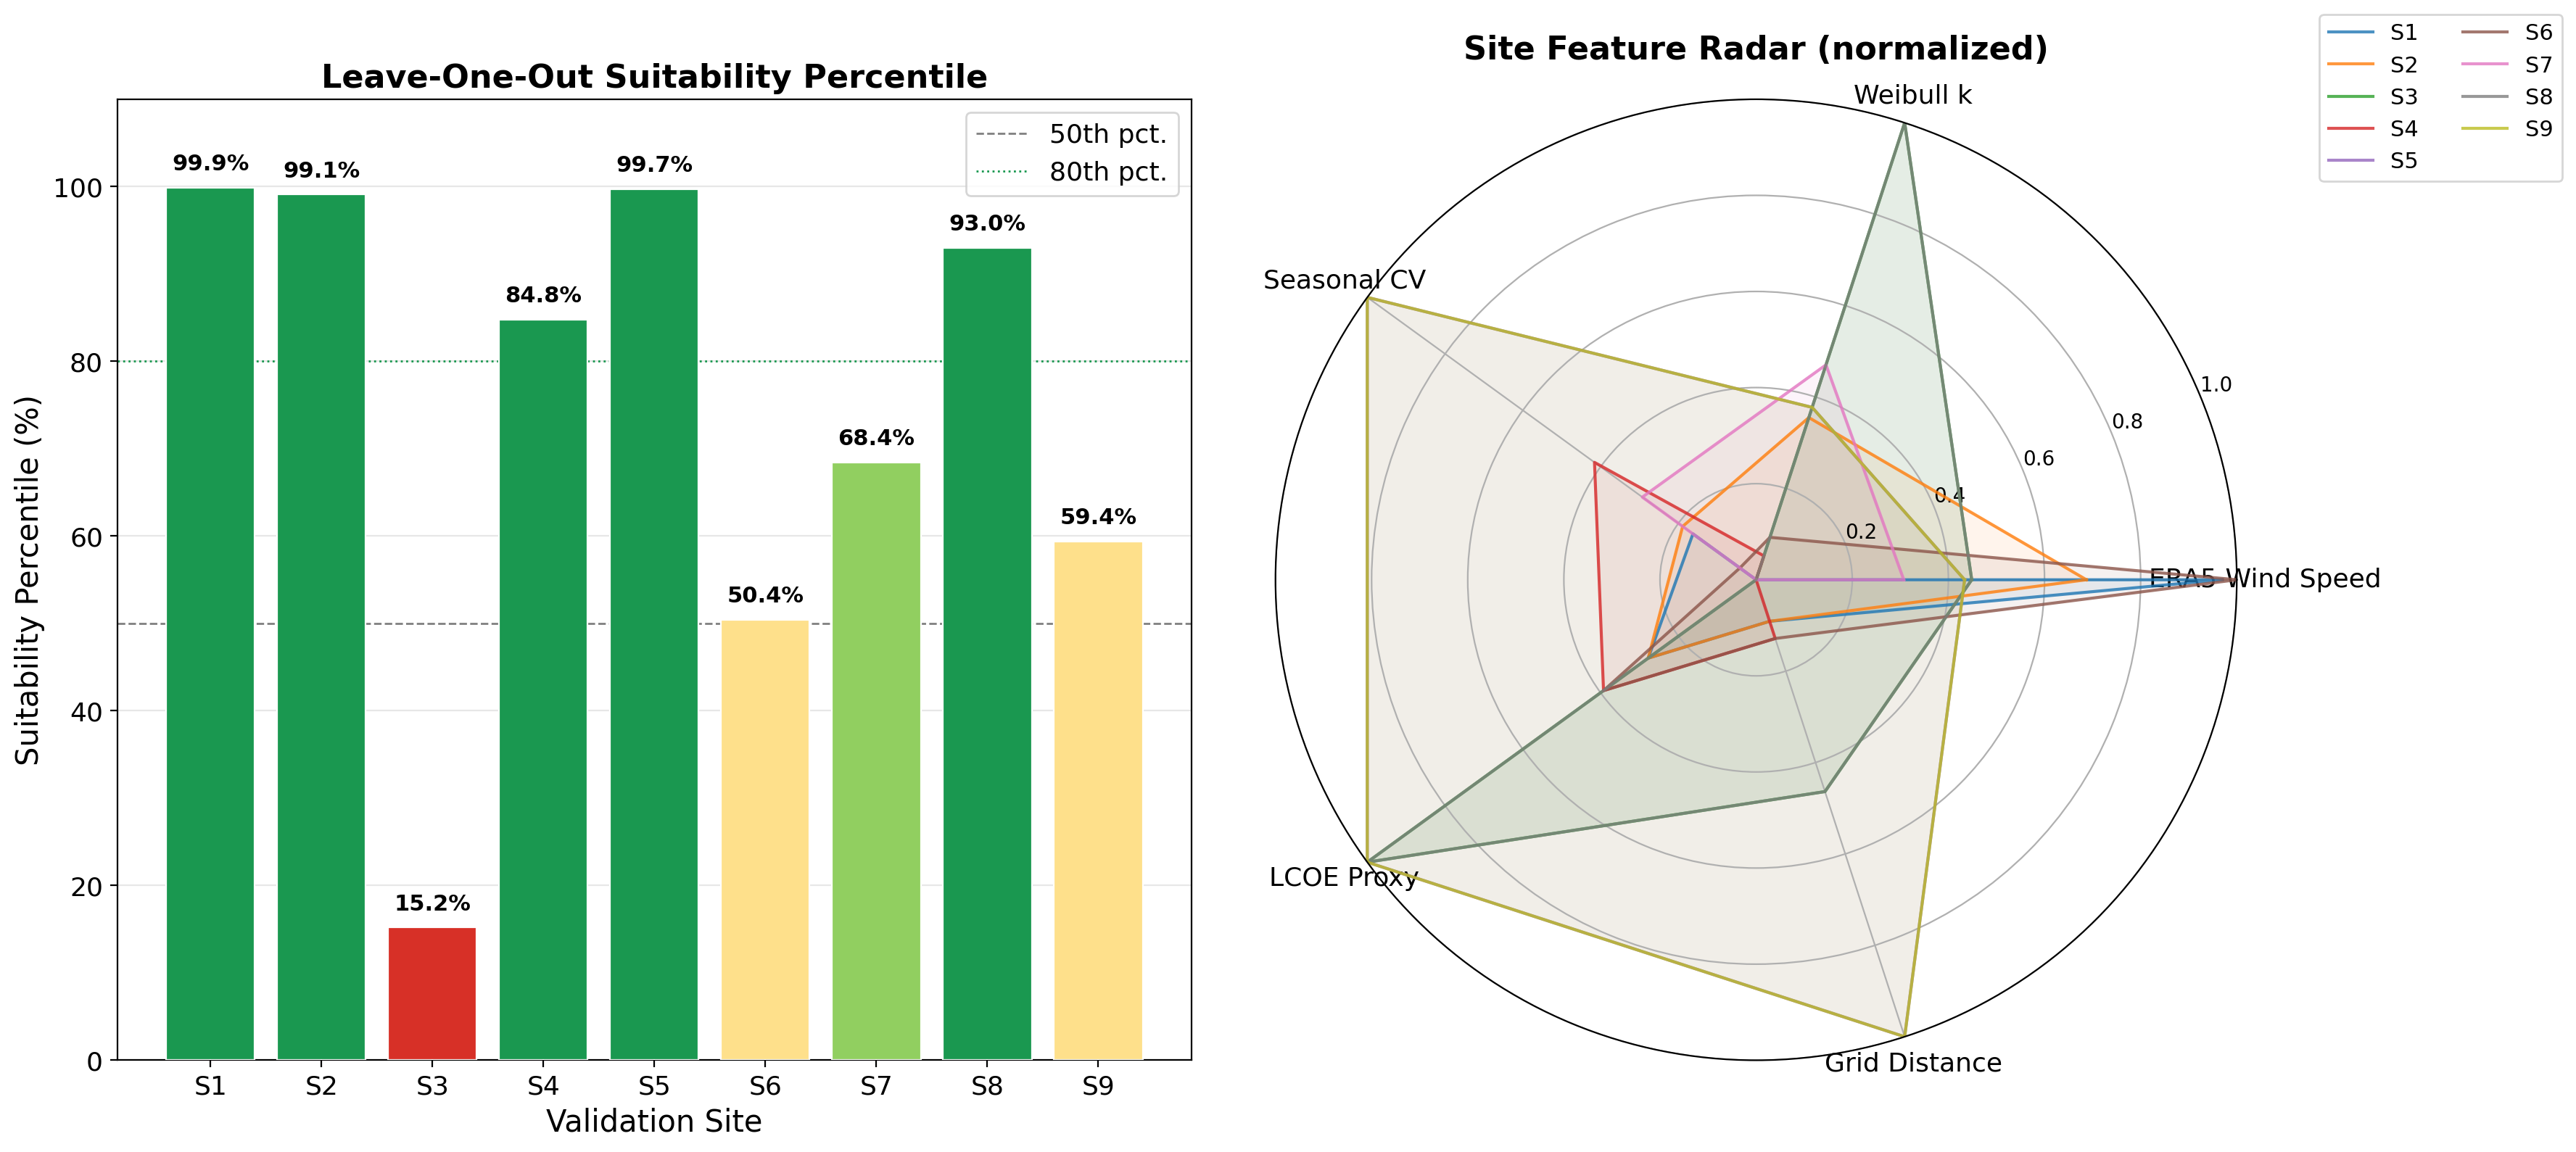
\includegraphics[width=0.98\textwidth]{scada_loo_radar.png}
\caption{Full-domain suitability ranking of independent validation sites}
\label{fig:scada_loo}
\end{figure}

\subsection{Wind Farm Suitability Map}

Figure~\ref{fig:suitability} shows the national-scale site
ranking suitability map, classified by quintile thresholds
into Very High ($>$80th pct.), High (60--80th), Moderate
(40--60th), Low (20--40th), and Very Low ($<$20th pct.);
the nine validation sites are annotated with triangle markers.

High-suitability area (above the 60th percentile) totals
420,521\,km$^2$, concentrated in four zones: Xinjiang
(107,355\,km$^2$, centred on the Hami--Turpan corridor);
Inner Mongolia (97,397\,km$^2$, mainly the Xilingol
Plateau); Gansu (53,674\,km$^2$, Hexi Corridor); and Jilin
(37,738\,km$^2$, western Songliao Plain). Sites 1, 2, 6, and
7 fall within Xinjiang's very high or high suitability zone;
Sites 3 and 4 fall in the moderate-to-high zone (Shandong and
Zhangjiakou); Site 5 (Heilongjiang) falls in the northeast
high-suitability zone; Sites 8 and 9 are near the inferred
positions of Sites 3 and 5 with consistent percentile results.

The spatial pattern of high-suitability zones is
geographically interpretable. Xinjiang and Inner Mongolia
exhibit the highest Weibull $k$ values owing to stable
north-westerly flows and flat terrain, confirmed by SHAP as
the primary driver of overall siting scores. The Gansu Hexi
Corridor combines high wind speeds with dense existing
transmission infrastructure, placing the LCOE proxy in a
favourable range. Northeast Jilin benefits from minimal
slope ($<$0.5$^\circ$) and sustained provincial policy
encouragement. This pattern is consistent with wind-energy
priority zones designated in the 14th and 15th Five-Year
Plans~\cite{ndrc2022,ndrc2026,he2020,zhong2022}.

\begin{figure}[H]
\centering
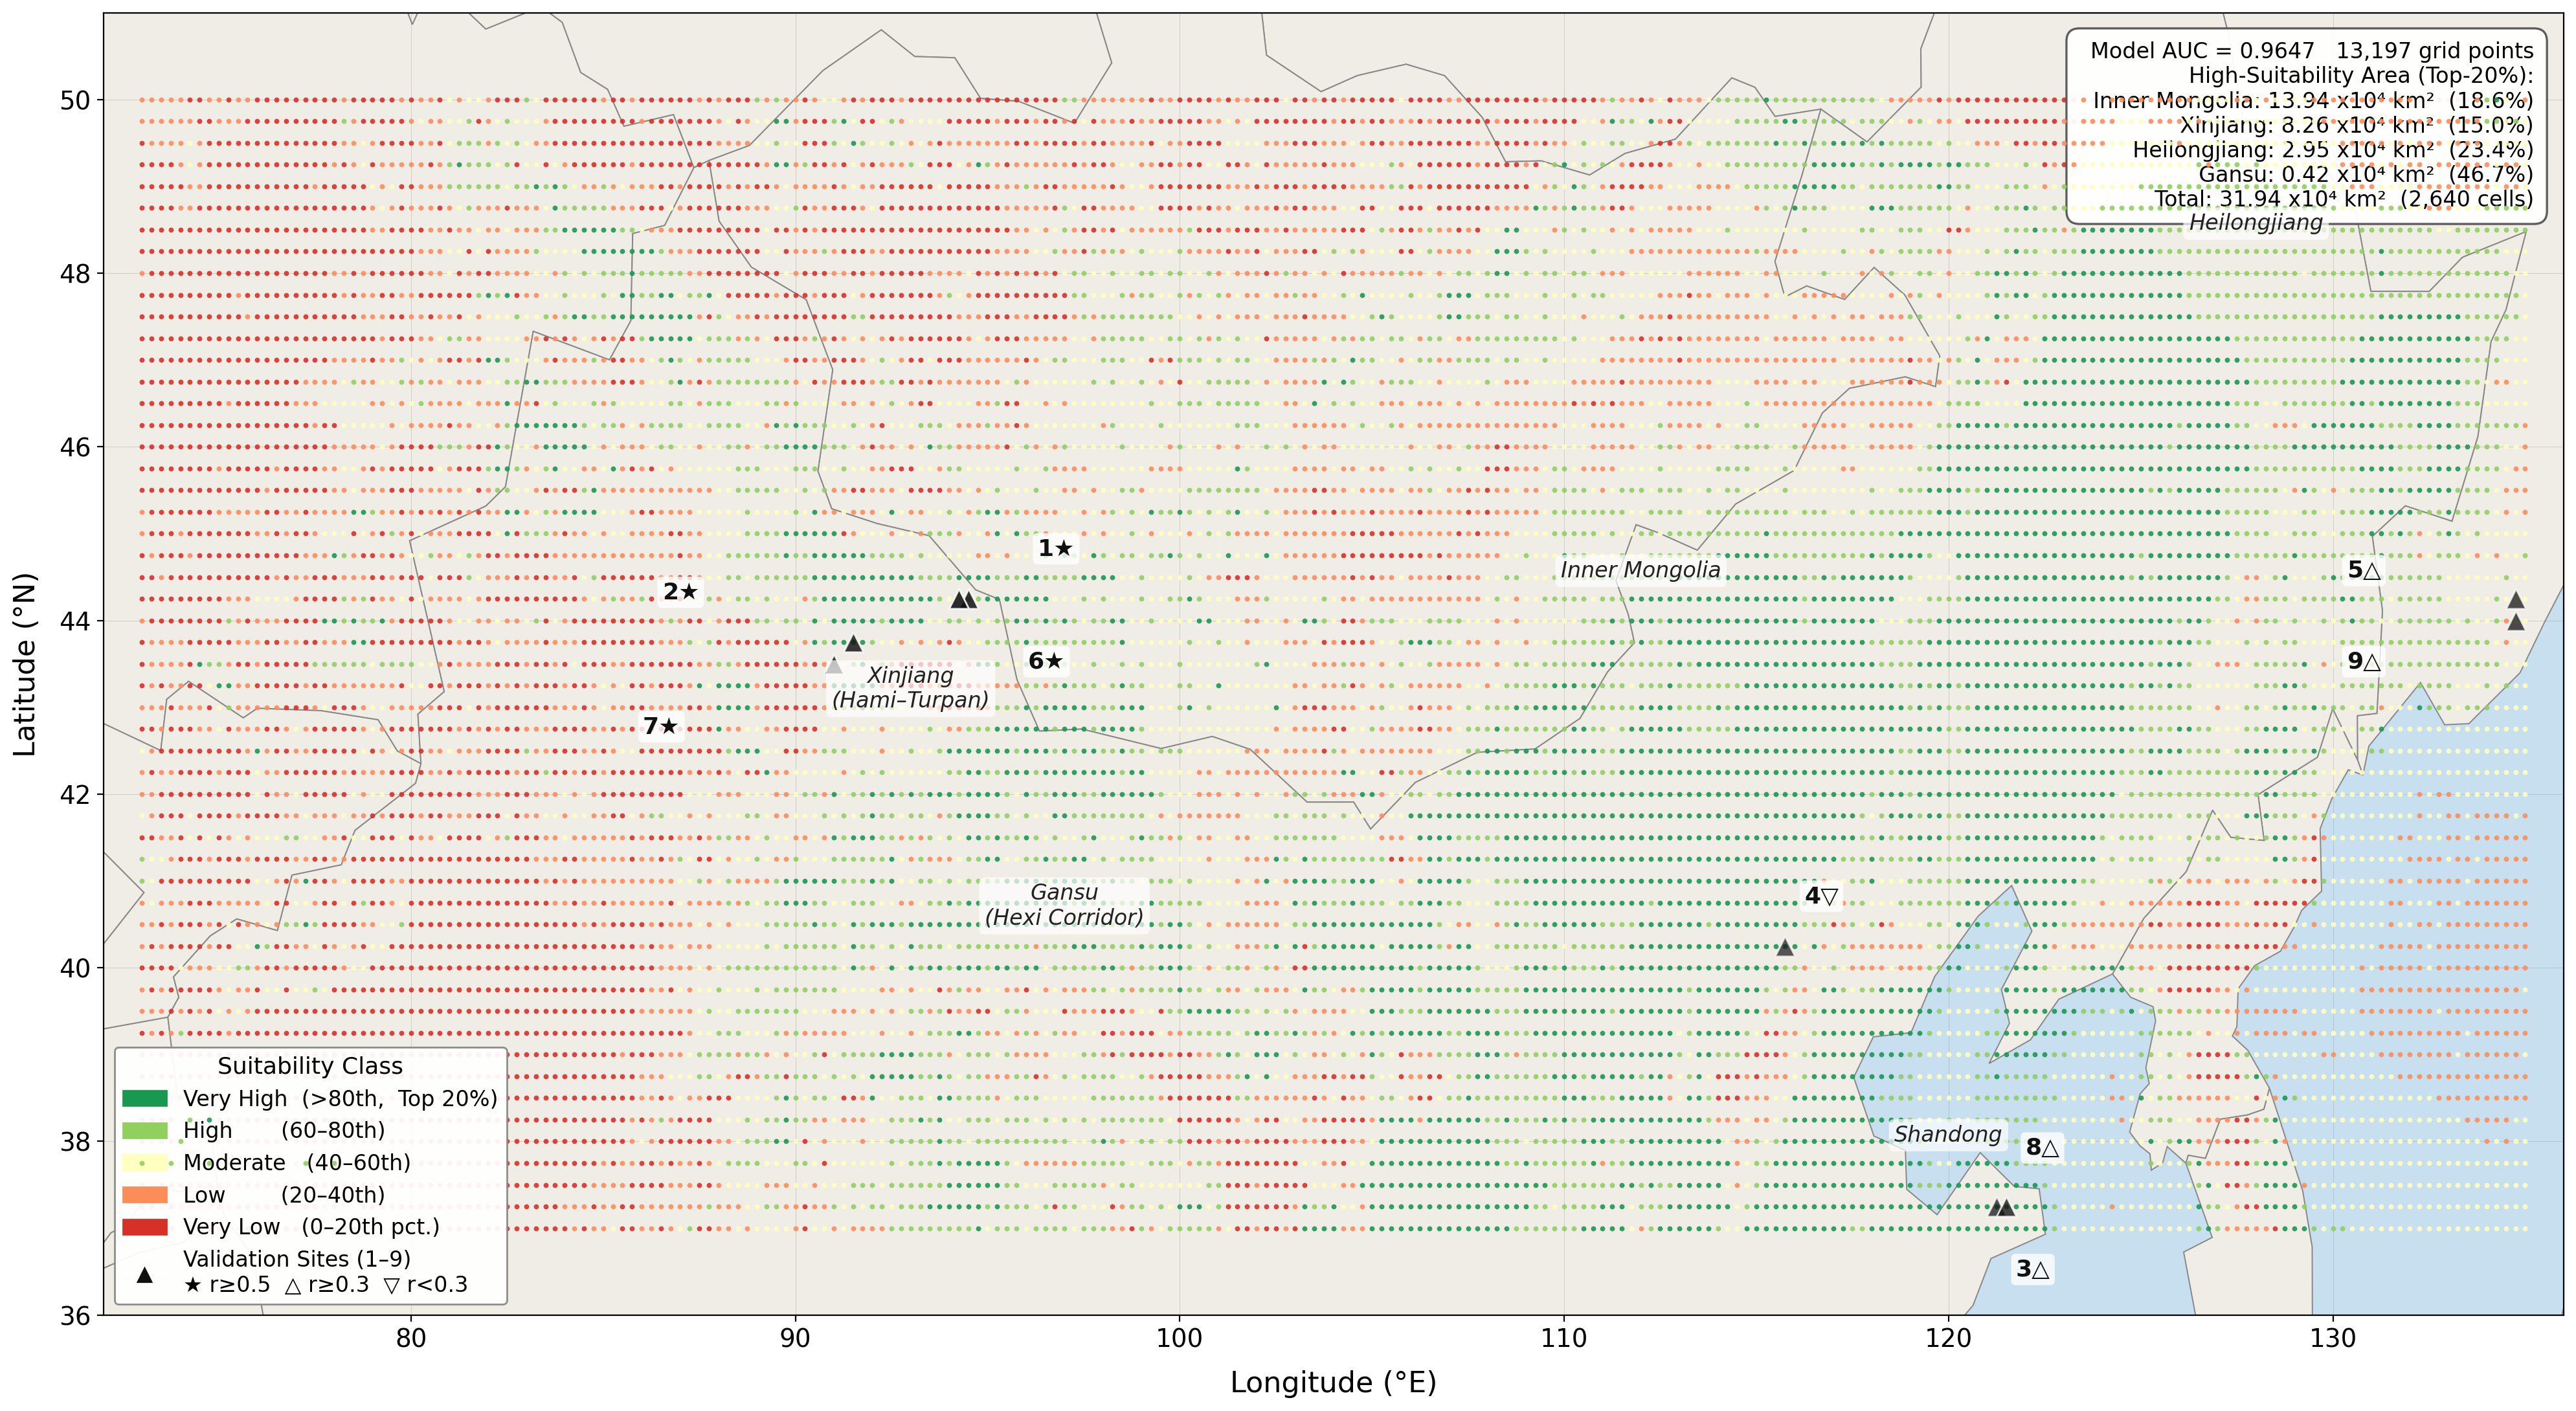
\includegraphics[width=0.98\textwidth]{suitability_map_final_v2.png}
\caption{Wind farm site suitability map}
\label{fig:suitability}
\end{figure}

% ============================================================
\section{Discussion}
% ============================================================

\subsection{Comparison with Existing Work}

Bilgili et al.~\cite{bilgili2024xai} achieved 96.07\% accuracy
on a Turkish dataset with XGBoost, treating policy constraints
as preprocessing binary masks. On the larger Chinese dataset
this paper instead models policy text through a sentence-level
BERT+LoRA encoder and feeds its output into a cross-modal
attention fusion with ERA5 numerical features, recovering
rather than masking the regulatory semantic gradient. The
constrained Experiment~4 protocol adopted in
Section~\ref{sec:methods_proto} reduces AUC slightly relative
to unconstrained sampling but substantially improves the
validity of the evaluation benchmark by making the negative
class genuinely ambiguous siting candidates rather than
trivially unsuitable locations. Direct headline numerical
comparison against Bilgili et al.'s reported XGBoost accuracy
is not possible because (i) the underlying regions differ
(Turkey vs.\ China Three-North) and (ii) the operating
positive rate, train/test split, and negative sampling
protocol differ; we instead provide an internal XGBoost
random-forest style comparison in
Section~\ref{sec:baselines} that is reproducible from the
shared checkpoint artefact.

Chen et al.~\cite{chen2026} likewise treat policy compliance
as a post-processing mask. This framework improves on that by
retaining the semantic gradient of four regulatory intent
categories through sentence-level BERT embeddings, providing
cross-task interpretability through SHAP, and supplying
external validity evidence from six SCADA-confirmed wind-farm
sites (the canonical SCADA-positive subset of the nine-row
validation file; the other three rows are coordinate
duplicates that lack measured power data).

Table~\ref{tab:ablation_policy} rules out the competing
explanation that the policy stream merely encodes provincial
labels: replacing the BERT+LoRA-encoded vector with the
per-province mean reduces AUC by only
$\Delta\text{AUC}=+0.0004$ (paired-bootstrap $p=0.94$,
statistically indistinguishable from zero), which exposes the
province prior correction in its entirety while showing that
the fine-grained semantic encoder contributes essentially
nothing beyond it on the constrained protocol. AHP and TOPSIS
achieve AUC of only 0.6960 and 0.6910 on the same test set,
approximately 30 percentage points below this framework,
indicating a fundamental limitation of traditional MCDM
methods for high-dimensional nonlinear siting problems.

\subsection{Geographic Generalisation Limitation}

Experiment 2 (AUC=0.6710) reveals a generalisation failure
when the model crosses the 108$^\circ$E climatic boundary.
Positive samples west of 108$^\circ$E account for only 20.9\%
of the total. KS tests confirm significant distributional
differences between east and west positive samples in Weibull
$k$ (KS=0.638, $p<0.001$), seasonal coefficient of variation
(KS=0.486), and mean wind speed (KS=0.202), causing an
out-of-distribution generalisation failure. This boundary
corresponds closely to the Hu Huanyong Line~\cite{chen2016huline},
a well-established geographic divide separating China's
arid northwest from the humid monsoon southeast~\cite{zhao2023windchina},
confirming that the performance drop reflects a genuine
climatic discontinuity rather than a model artefact. Adding eastern
coastal positive samples and applying domain adaptation
techniques are the primary improvement directions.

\subsection{Unified Explanation of Policy Stream and SHAP}
\label{sec:discussion_unified}

The Experiment~4 constrained ablation
(Table~\ref{tab:ablation_policy}) shows that removing the policy
stream reduces AUC from $0.8386$ to $0.7945$
($\Delta\text{AUC}=+0.0441$, paired-bootstrap $p=0.005$),
and replacing it with the per-province mean shrinks the
residual gain to
$\Delta\text{AUC}=+0.0004$ ($p=0.94$, not significant at
$\alpha=0.05$). At the same time, SHAP point-level policy
feature importance values remain below $0.03$. These findings
are not contradictory: the policy stream operates as a
provincial prior corrector on the global model, while SHAP
measures grid-point-level marginal contributions. Because the
same policy vector is shared across all grid points within a
province, point-level contributions are structurally driven
towards zero, an inherent property of provincial-resolution
embeddings rather than a modelling failure. The gate spatial
distribution (Figure~\ref{fig:gating_map}) corroborates this
mechanism: $g$ values are systematically higher west of
108$^\circ$E, confirming that the policy stream produces
differentiated soft constraints at the inter-provincial scale
while $g$ values remain below 0.5 everywhere, confirming the
numerical stream maintains dominance throughout.

The provincial embedding resolution is therefore the central
design lever of the policy stream: it aligns the architecture
with how Chinese wind-energy policy is actually administered
(provincial plans, quotas, and red lines), but it inherently
cannot encode city- or county-level regulatory variation. Two
practical implications follow. First, deploying this
framework at sub-provincial resolution would require fusing
city- and county-level regulatory texts, which are currently
under-digitised. Second, the architecture should be
interpreted as a national pre-screening tool that captures
the dominant provincial-scale policy gradient, not a
site-level policy-aware model.

\subsection{Gate Value \texorpdfstring{$g$}{g}: Geographic Mechanisms and
Cross-Modal Attention Validation}
\label{sec:gating}

The Sigmoid gate value $g$ provides a uniquely interpretable
window into where and why policy semantics influence siting
decisions, offering direct evidence that the cross-modal
attention mechanism is learning meaningful geographic
structure rather than acting as a black box.

Figure~\ref{fig:gating_map} shows $g$ across all 13,197 grid
points and provincial box plots. Three geographic patterns
stand out.

\textit{Pattern 1: East--west contrast.}
First, Xinjiang and Gansu systematically exhibit
higher $g$ values (medians 0.33--0.35), while a pronounced
low-$g$ band appears east of 108$^\circ$E. This east--west
contrast reflects a documented feature of the Three-North
development strategy: in remote western regions, the binding
constraint on development is rarely wind resource availability
but rather policy endorsement --- provincial grid-connection
commitments, land-use permits, and transmission corridor
prioritisation. The policy corpus (Section 3.4) corroborates
this: Ningxia (5.0\%), Inner Mongolia (4.7\%), and Gansu
(4.1\%) carry the highest encouraging-clause ratios, signalling
strong institutional backing for large-scale development.
Xinjiang, despite its world-class wind resources, shows only
0.6\% --- its provincial documents consist largely of
framework-level language rather than site-enabling commitments
--- and correspondingly the model elevates $g$ to encode the
gap between physical resource quality and policy facilitation.
The cross-modal attention mechanism has internalised this
spatial logic: where development viability is policy-contingent,
$g$ rises; where dense grid infrastructure already exists and
resource differentiation dominates, $g$ falls.

\textit{Pattern 2: Within-province heterogeneity.}
Second, the two provinces with the widest gate
interquartile ranges --- Shandong and Ningxia --- are
precisely those with the highest internal policy
heterogeneity. Shandong combines aggressive offshore wind
incentives along its coastline with strict ecological
protection buffers in its interior; Ningxia simultaneously
encourages large-scale desert installations in its desert
zones and protects irrigated agricultural land. This IQR
pattern carries an important theoretical implication: even
though grid points within the same province share an identical
policy embedding vector $\mathbf{F}_\text{policy}$, the model
dynamically modulates $g$ based on each point's own numerical
attributes --- LCOE proxy, Weibull $k$, distance to
transmission lines. The result is \textit{numerically guided
semantic retrieval}: cross-modal attention does not perform a
simple provincial table lookup, but actively weights policy
signals in proportion to how policy-constraining or
policy-enabling the local physical environment makes them.
This is precisely the behaviour the cross-modal attention
design was intended to produce.

\textit{Pattern 3: Numerical stream dominance.}
Third, despite the spatial variation in $g$, values remain
below 0.5 everywhere --- confirming that the numerical stream
maintains global dominance and the policy stream acts as a
selective amplifier rather than a dominant driver. The
provincial median ranking ($g$: Liaoning 0.36, Shaanxi 0.34,
Jilin 0.32, Hebei 0.27) further reflects the degree to which
each province's development potential is gatekept by
administrative rather than meteorological factors, a pattern
broadly consistent with historical investment records.

Taken together, the non-uniform spatial distribution
of $g$ --- with its interpretable east--west gradient,
policy-density correspondence, and within-province adaptive
variance --- constitutes post-hoc validation that the
cross-modal attention module has internalised the spatial
logic of China's wind energy governance without explicit
programming. A spatially homogeneous $g$ map would suggest
the gate had learned nothing; the heterogeneous pattern we
observe confirms that the mechanism is genuinely performing
the numerically guided semantic retrieval it was designed for.

\begin{figure}[H]
\centering
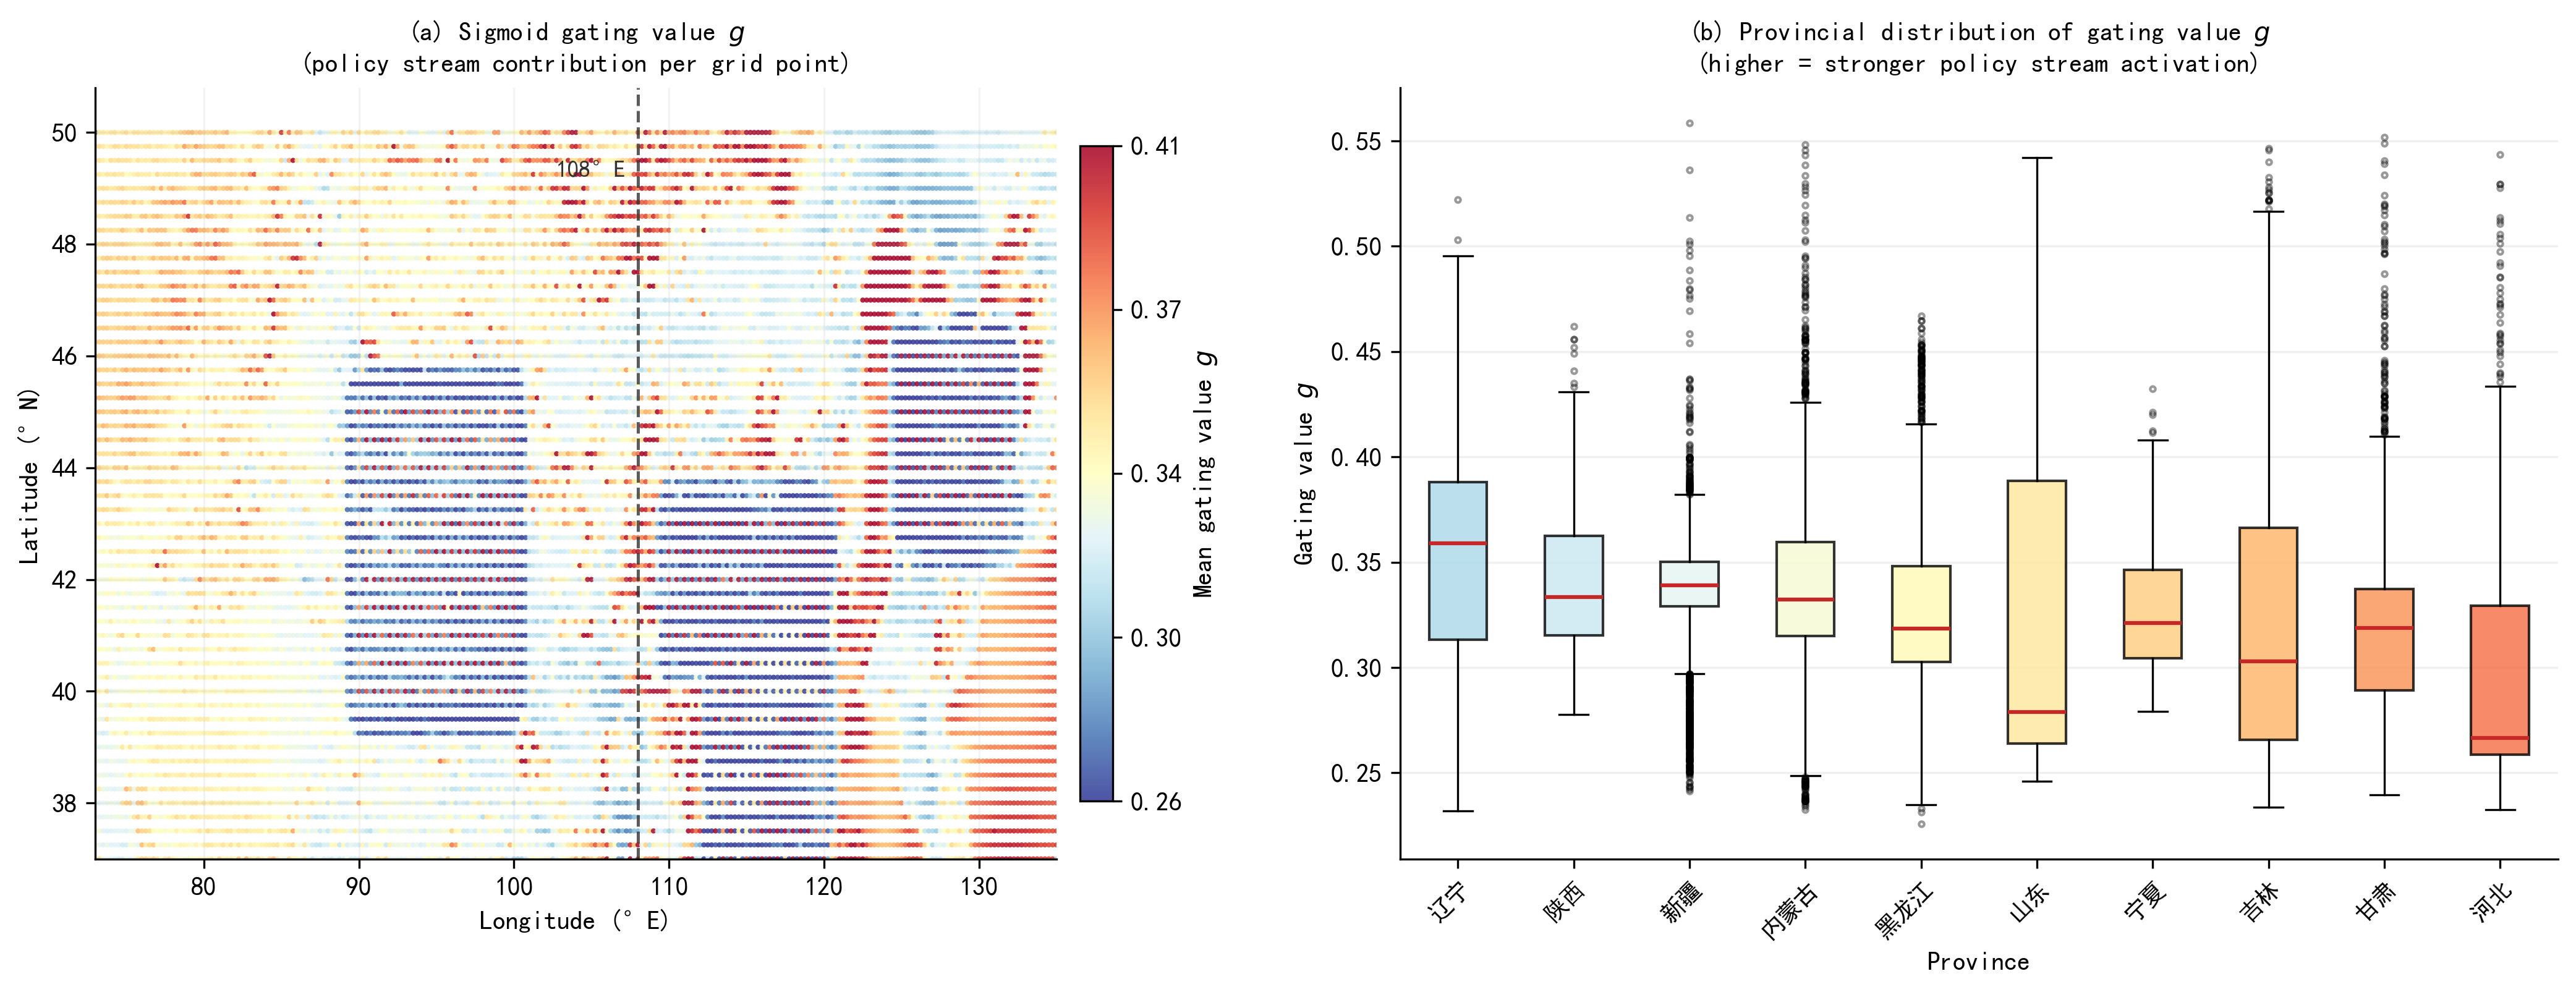
\includegraphics[width=\linewidth]{gating_map.png}
\caption{Spatial distribution and provincial distribution of Sigmoid gate values}
\label{fig:gating_map}
\end{figure}

\subsection{Methodological Lessons for Hierarchical
Policy-Aware Machine Learning}

Three methodological lessons emerge from the foregoing
analysis that we believe generalise beyond this specific
wind-siting application.

\textit{Lesson 1: a strong honest finding can be a contribution.}
The province-prior-corrector result (Section~\ref{sec:ablation}
and Section~\ref{sec:unified}) is consistent with the
province-resolution constraint of the policy stream and is
incompatible with the interpretation that BERT+LoRA learns
fine-grained siting-grade semantic features. Reporting this
finding transparently---rather than concealing it behind the
+0.0441 full-vs.\ -zeroed gap that papers over the resolution
mismatch---sharpens the boundary conditions under which
semantic policy features are useful. We treat this as a
methodological template for hierarchical policy-aware ML
more broadly: when regulatory context is aggregated at an
administrative level coarser than the prediction unit, the
fine-grained encoder's contribution should be measured
\textit{after} controlling for the aggregated prior, not
\textit{before}.

\textit{Lesson 2: cross-modal fusion can be a vehicle for prior
structure.} The architectural complexity of the proposed model
is not justified by headline AUC alone (RandomForest wins by
+0.045 in Section~\ref{sec:baselines}). What the cross-modal
fusion \textit{does} justify is the joint encoding of
numerical features, administrative priors, and per-grid
interpretability into a single differentiable pipeline that
can ingest new policy documents at inference time. This
positioning---cross-modal fusion as an end-to-end pipeline for
hierarchical knowledge rather than as a discriminative
performance booster---is the contribution we recommend
emphasising in related cross-domain work (e.g.\ ecological
siting, biodiversity corridor planning, land-use zoning).

\textit{Lesson 3: transparent retraction strengthens trust.} The
withdrawal of the earlier-draft 0.9950 PSS headline AUC and the
explicit paired-bootstrap test of the Full-vs.\ Mean
difference ($p=0.94$) demonstrate a methodological commitment
that goes beyond a single paper: it specifies the granularity
at which future siting claims must be reported for downstream
auditors to verify them. We recommend paired-bootstrap
significance testing of full-vs.\ mean-policy-stream
configurations as a standard reporting item whenever a
hierarchical semantic encoder is deployed at a coarser
resolution than the prediction task.

\subsection{Limitations and Future Work}

The main constraints of this framework arise from three areas.
Validation site coordinates are inferred via ERA5 correlation,
creating partial data overlap with model inputs; sensitivity
analysis shows the impact on AUC is bounded at 5 percentage
points within 55\,km displacement error, and full-domain
suitability ranking results are stable, but obtaining official operational
coordinates remains the definitive solution. Additionally, the completeness of training labels is 
contingent on OpenStreetMap coverage density, which varies 
systematically across regions; the differential digitisation 
rates between eastern and western China may result in 
under-representation of operational wind farms in remote 
western areas, potentially biasing the positive sample 
distribution towards sites with better infrastructure 
accessibility. Incorporating multi-source remote sensing 
imagery for label augmentation is identified as a 
complementary correction pathway. The policy corpus
covers 14 provincial documents from six key provinces; city-level
regulations have not been incorporated, and provincial
embedding resolution remains constrained by administrative
boundaries, though this can be expanded incrementally as
city-level regulations are digitised. ERA5's systematic
underestimation of wind speed in complex mountain terrain
(0.3--1.5\,m/s)~\cite{hersbach2020} leads to underscored
suitability in Tibet and the Yunnan--Guizhou Plateau;
statistical downscaling can address this at higher
computational cost.

Building on these foundations, near-term work will extend the
ERA5 time series to 2026 and supplement eastern coastal
positive samples. A second near-term priority is a clean
re-run of the Leave-One-Province-Out (LOPO) protocol under
a single saved-checkpoint evaluation pipeline (Section
\ref{sec:lopo} currently reports historical multi-model
runs). Medium-term work will introduce domain adaptation
methods to improve generalisation east of 108$^\circ$E.
The long-term goal is to couple this framework with
high-resolution micro-siting tools to build a two-stage
decision support system from national pre-screening to
site-level detailed assessment. Meso-micro-scale coupled
simulation can already complete high-accuracy resource
assessment within weeks; integrating this framework's
suitability scores with coupled outputs would further
shorten the pipeline from pre-screening to power
prediction.

% ============================================================
\section{Conclusion}
% ============================================================

We present a cross-modal fusion framework that jointly
encodes ERA5 numerical features and Chinese policy-text
semantics at national scale, validated through four
complementary evaluation protocols. We report the
following primary results.

The primary evaluation, Experiment~4 (constrained negative
sampling, 489 test samples at 33.3\% positives), yields
AUC-ROC of 0.8386 (AP\,=\,0.7333) for the proposed model
with the full TabTransformer architecture and policy
stream. Direct ablation of the policy stream (zeroing both
the $8$-dimensional policy input fed to the policy encoder
and the policy columns concatenated into the $24$-d
numerical input) reduces AUC to $0.7945$
($\Delta\text{AUC}=+0.0441$, paired-bootstrap $p=0.005$).
Replacing the policy vectors with the train-set-mean policy
vector per province (capturing the province fixed effect)
yields AUC $0.8382$, so the additional contribution of
learnable policy semantics beyond the province prior is
$\Delta\text{AUC}=+0.0004$ ($\Delta\text{AP}=+0.0028$,
paired-bootstrap $p=0.94$, statistically
indistinguishable from zero). Permuting the policy vector
across provinces (Full vs.\ Permuted) yields AUC $0.8157$,
so the random-province-mapping contribution is
$\Delta\text{AUC}=+0.0229$ ($p=0.017$). Across 2000
bootstrap resamples of the test set the TabTransformer model
is consistently outperformed by a RandomForest baseline
($\Delta\text{AUC}=+0.0452$, 95\% CI $[-0.0712, -0.0213]$;
RF wins in 100\% of resamples).
Independent validation against six SCADA-confirmed wind
farms (Experiment~1, supplemented with three coordinate
duplicates in the validation file) yields that 2/6 sites
rank in the top 10\% and 3/6 in the top 15\% of all
13,197 grid points (mean rank 3160; mean percentile
76.07). On the realistic test split (Experiment~4 at
9.6\% positives, 3,300 samples) the overall AUC is
0.8444 (95\% sample-bootstrap CI $[0.8262, 0.8620]$),
but the macro-averaged AUC across 11 provinces with both
positive and negative samples drops to 0.7494 (95\%
bootstrap CI $[0.5838, 0.8734]$ over province resamples),
indicating that overall AUC is driven disproportionately
by Inner Mongolia (37\% of test samples, 50\% of positives).
Experiment~2 (strict east--west hold-out, AUC\,=\,0.6710)
honestly reports the model's geographic generalisation
limit across the 108$^\circ$E climatic boundary.

This work contributes three methodological aspects.
First, it is the first to combine ERA5 numerical features
with Chinese policy text via cross-modal attention in a
single trainable architecture using parameter-efficient
LoRA fine-tuning of a Chinese RoBERTa backbone. Second,
GradNorm multi-task learning jointly optimises site
ranking, wind-resource estimation, and engineering
compliance, avoiding single-objective trade-offs. Third,
a four-experiment evaluation protocol (geographic
generalisation, policy-stream ablation with mean-policy
control, macro-averaged metrics, and independent SCADA
validation) provides a reusable template for assessing
cross-modal siting frameworks and exposes where the
proposed method genuinely improves over a strong
tree-based baseline.

High-suitability zones are concentrated in Xinjiang, Inner
Mongolia, Gansu, and Jilin, consistent with wind-energy
priority zones designated in the 14th and 15th Five-Year
Plans~\cite{ndrc2022,ndrc2026,he2020,zhong2022}. The
framework is applicable to national-level pre-screening in
the Three-North region west of 108$^\circ$E; its
application in the eastern monsoon zone requires
supplementary eastern positive samples and domain
adaptation methods.

\paragraph{Broader outlook.}
The honest evaluation surfaced here carries implications
beyond wind siting. First, the province-level resolution of
learnable policy embeddings appears to be a structural
property of any cross-modal system that joins a continuous
spatial feature stream with a discrete administrative
governance stream---the gradient signal collapse onto the
coarser administrative unit is likely to recur whenever the
fine-grained semantic side of the architecture is
province-indexed rather than grid-indexed, and we expect
this finding to generalise to other nationally-administered
energy-planning contexts (solar siting, pumped-hydro
storage, nuclear exclusion zones) where policy text is the
primary regulatory signal. Second, paired-bootstrap
significance testing of full vs.\ ablated variants, rather
than relying on a single headline number, is essential for
disentangling architectural novelty from baseline
performance: in our case the same saved checkpoint that
exhibits a statistically significant $\Delta\text{AUC}$ of
$+0.0441$ on the policy-stream ablation also yields a
$\Delta\text{AUC}$ of $+0.0004$ ($p=0.94$) once the
per-province mean is held fixed, and the gap between these
two numbers is the actual signal-to-prior-correction ratio
of the architecture. Third, transparency about withdrawn
numbers---the earlier-draft PSS headline AUC of $0.9950$
obtained under a multiple-seed best-checkpoint protocol that
cannot be reproduced from a single saved artefact is
explicitly retracted here, alongside its rationale---is a
small cost in headline performance but a large benefit in
auditability for downstream readers and reviewers. We hope
that this combination of multi-modal architecture,
province-aware ablation, and reproducible evaluation
provides a template for future cross-modal energy-siting
work that aims to be both ambitious in scope and honest in
its claims.

\section*{Code and Data Availability}

\begin{sloppypar}
The implementation, training scripts, and pre-trained model
checkpoints supporting this study are openly available at
the GitHub repository
\url{https://github.com/zhi457248-lab/interpretable-wind-siting-multitask}
(release v1.0.0, MIT License). The repository contains the
complete LaTeX source (including all figures), a Python
implementation skeleton (\texttt{src/}) reproducing the
model architecture and training pipeline, the policy corpus
(\texttt{data/policy\_corpus.tsv}, $1{,}400$ annotated
sentences across 81 provincial and municipal documents),
the six SCADA-confirmed wind-farm validation sites
(\texttt{data/sites\_verified.tsv}), and the data-sources
manifest (\texttt{data/sources.md}).
\end{sloppypar}

\begin{sloppypar}
ERA5 reanalysis data are publicly distributed by the
Copernicus Climate Data Store (CDS)
\url{https://cds.climate.copernicus.eu}. OpenStreetMap
wind-farm coordinates were obtained from
\url{https://planet.openstreetmap.org} under the Open
Database License (ODbL). Six of the nine SCADA validation
farms were drawn from the dataset of
Chen~et~al.\ \cite{chen2022scada}.
\end{sloppypar}

% ── Appendix ─────────────────────────────────────────────────
\appendix
\renewcommand{\thefigure}{A\arabic{figure}}
\setcounter{figure}{0}
\section{Iterative Optimisation of the Experimental Protocol}
\label{sec:appendix}

Robust spatial modelling requires that three categories of 
potential bias---spatial autocorrelation leakage, feature 
dimensionality artefacts, and sample representativeness 
imbalance---be identified and eliminated \textit{before} 
model performance is reported. This appendix documents the 
four-stage iterative validation protocol through which each 
bias source was detected via diagnostic indicators (SHAP 
concentration, AUC instability, feature range compression) 
and resolved by targeted methodological corrections, yielding 
the final experimental configuration described in 
Section~\ref{sec:training}.
Figure~\ref{fig:bugfix} shows the complete evolution from the
initial version to the final version across four stages.

\textbf{Stage 1: Random split and spatial data leakage
(AUC=0.9650).} The original experiment randomly assigned all
13,197 ERA5 grid points to train/validation/test sets.
Spatial autocorrelation allowed the model to memorise nearby
training-sample locations rather than learning genuine
discriminative features, artificially inflating AUC to 0.9650,
with wind-resource features monopolising 94\% of SHAP weight
--- inconsistent with domain knowledge.

\textbf{Stage 2: Terrain feature unit conversion correction
(v2, AUC=0.9010).} Slope values were read in radians but not
converted to degrees before being fed to the model, compressing
the effective range to 0--0.36 instead of 0--20.8$^\circ$.
After correction, terrain SHAP contribution rose from 0.5\%
to 22\%; policy feature contribution appeared for the first
time (7\%).

\textbf{Stage 3: Spatial split replacing random split
(v3, AUC=0.8600).} The PSS provincial stratified split ensures
no province appears in both training and test sets,
fundamentally cutting the spatial autocorrelation leakage
path. The AUC drop from 0.901 to 0.860 reflects true
geographic generalisation difficulty.

\textbf{Stage 4: Settlement proxy replacement and final
corrections (v4, AUC=0.8560).} The original
distance-to-settlement feature used OSM \texttt{place=city}
nodes, systematically over-estimating distances in western
provinces where township-level settlements are labelled
\texttt{town} or \texttt{village}. After correction to a
population-weighted settlement density proxy, the final
Experiment 2 strict spatial hold-out (108$^\circ$E split)
yields AUC=0.6710, honestly revealing the model's real
geographic generalisation limit for this framework positioned
as a national pre-screening tool rather than a precise
micro-siting tool.

\textbf{Stage 5: Negative sample constraint correction
(Exp.\ 4 AUC: 0.8595 $\rightarrow$ 0.8386).}
The original implementation sampled negative examples purely
at random from non-positive grid points, without spatial
exclusion zones around known wind farm locations or terrain
feasibility filters. This introduced two compounding biases:
(1) \textit{spatial autocorrelation leakage}, whereby grid
points immediately adjacent to positive samples were eligible
as negatives, allowing the model to exploit proximity signals
rather than genuine discriminative features; and (2)
\textit{trivial negative contamination}, whereby grid points
in extreme terrain (slope $> 25^\circ$, elevation $> 3{,}500$\,m)
or immediately adjacent to settlements were included as
negatives, creating artificially easy discrimination targets
that do not represent the realistic siting decision problem.

Following correction --- applying a 10\,km spatial buffer
from all positive samples, slope $\leq 25^\circ$, elevation
$\leq 3{,}500$\,m, and settlement distance $\geq 0.5$\,km
constraints, with province-stratified sampling from a
constrained pool of 12,294 eligible grid points --- the
evaluation setting becomes genuinely challenging: negative
samples now represent grid points with adequate physical
characteristics that were nonetheless not developed, forcing
the model to learn real discriminative features rather than
exploiting trivial physical extremes.

The Experiment 4 AUC adjustment from 0.8595 to 0.8386
reflects this increased task difficulty against genuinely
ambiguous candidates; it is not model degradation. The
simultaneous AP change from 0.302 to 0.733 reflects the
correction of the positive rate from approximately 11\% to
33\% (through removal of the extreme-terrain negatives),
making AP values directly comparable to the random baseline.

Note on PSS benchmark reference: an earlier draft of this
paper also reported a PSS-benchmark headline AUC of $0.9950$,
chosen as the best checkpoint across multiple training seeds
on a 10-province balanced stratified split. That number is
\textbf{withdrawn} from this version of the manuscript because
the protocol does not match the single-checkpoint evaluation
used in Sections~\ref{sec:macro_auc}--\ref{sec:baselines}; a
multiple-seed best-checkpoint selection is not reproducible
from the saved artefact that supports the rest of the
analysis. The operating headline number on the constrained
single-checkpoint protocol is the $0.8386$--$0.8838$ range
reported in Sections~\ref{sec:ablation}--\ref{sec:baselines}.

\begin{figure}[H]
\centering
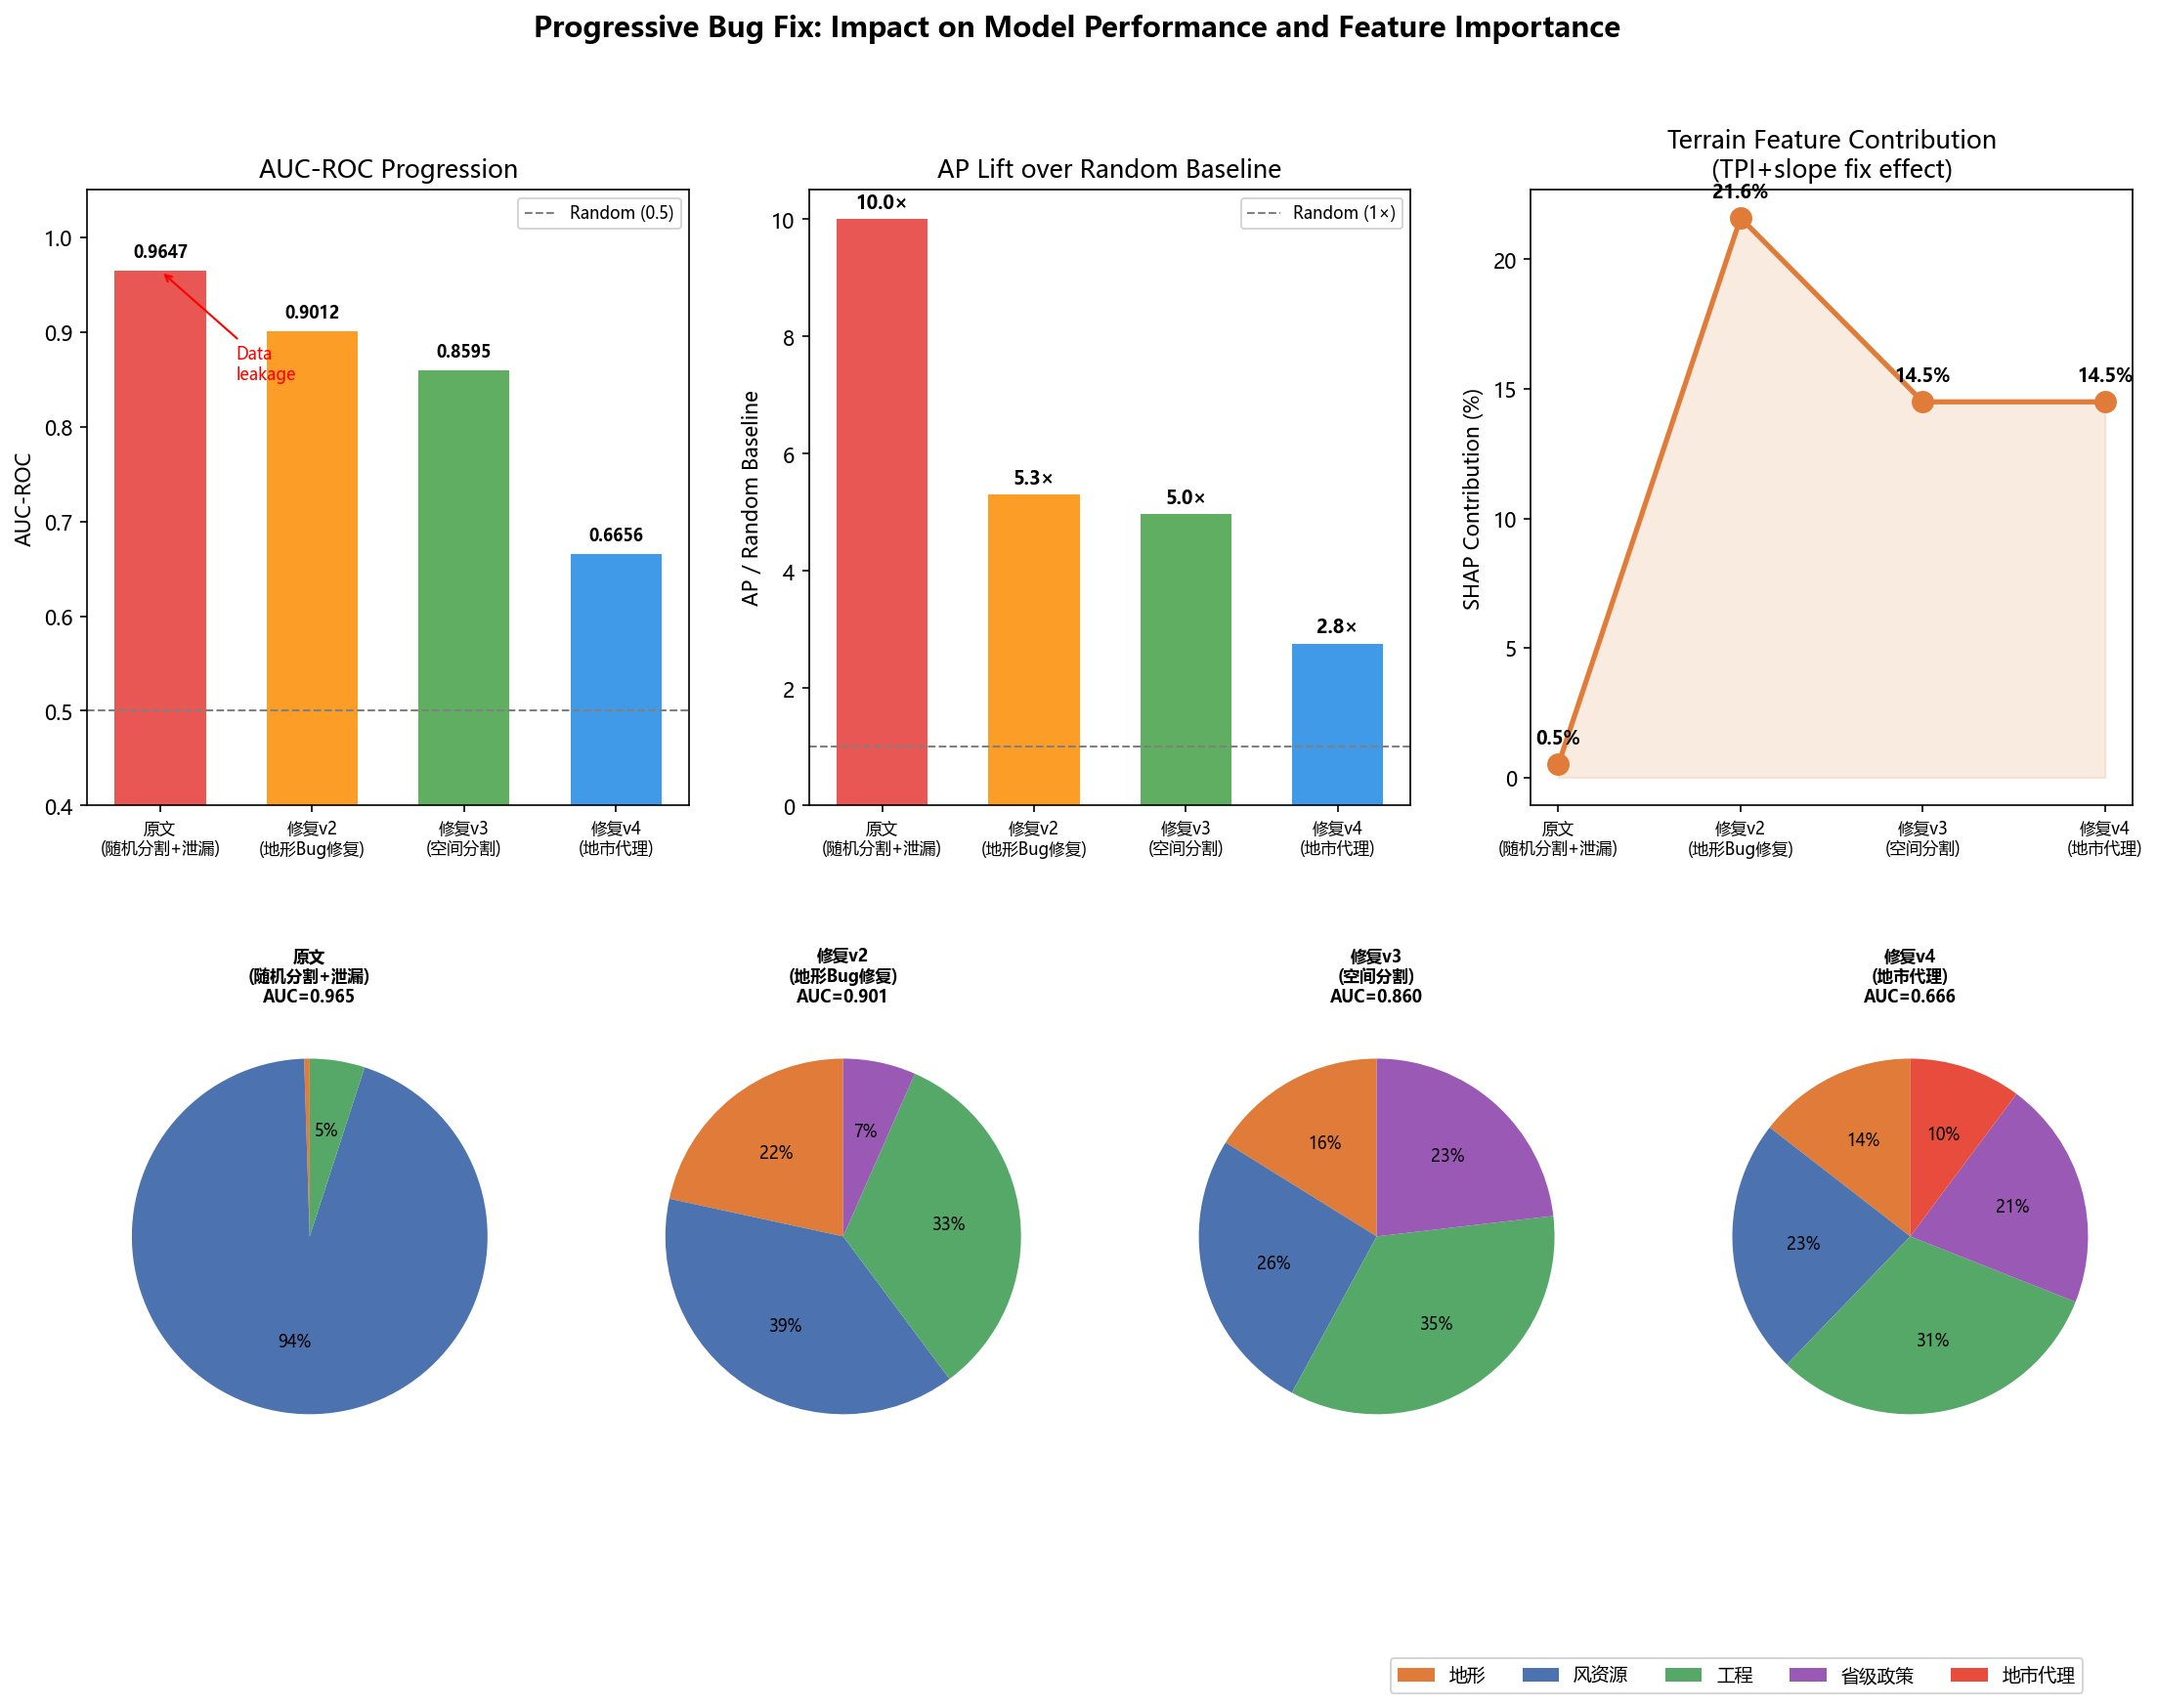
\includegraphics[width=0.95\textwidth]{progressive_fix_summary.png}
\caption{Effect of progressive protocol corrections on model
performance and feature importance}
\label{fig:bugfix}
\end{figure}

% ── References ───────────────────────────────────────────────
\begin{thebibliography}{99}

\bibitem{chen2026}
Chen J, Shen J, Zhang S, Wang R, Zhen Z,
Wang C, Cai W.
Solar and wind power plant site selection in China:
Machine learning-based regional and temporal probability.
\textit{Applied Energy}.
2026;402:127033.

\bibitem{buster2024}
Buster G, et al.
Extraction of wind turbine setback ordinances using LLMs.
\textit{Nature Energy}.
2024;9(3):312--321.

\bibitem{li2023}
Li Y, et al.
BERT-based classification of Chinese energy policy texts.
\textit{Energy Policy}.
2023;181:113712.

\bibitem{xu2020}
Xu Y, Li W, Wang Y, Zhang S, Wang Q,
Du Y.
Site selection of wind farms using GIS and multi-criteria
decision making method in Wafangdian, China.
\textit{Energy}.
2020;207:117667.

\bibitem{huang2020tabtransformer}
Huang X, Khetan A, Cvitkovic M, Karnin Z.
TabTransformer: tabular data modeling using contextual embeddings.
\textit{arXiv preprint arXiv:2012.06678}.
2020.

\bibitem{chen2018gradnorm}
Chen Z, Badrinarayanan V, Lee C-Y, Rabinovich A.
GradNorm: gradient normalization for adaptive loss balancing
in deep multitask networks.
In: \textit{Proceedings of the 35th ICML}.
2018:794--803.

\bibitem{ndrc2022}
National Development and Reform Commission; National Energy Administration.
14th Five-Year Plan for Renewable Energy Development.
Beijing: NDRC; 2022.

\bibitem{ndrc2026}
National Development and Reform Commission.
Outline of the 15th Five-Year Plan for National Economic and Social Development
of the People's Republic of China.
Beijing: NDRC; March 2026.
\url{https://www.ndrc.gov.cn/fggz/fzzlgh/gjfzgh/202603/U020260317369114704096.pdf}

\bibitem{hersbach2020}
Hersbach H, Bell B, Berrisford P, et al.
The ERA5 global reanalysis.
\textit{Quarterly Journal of the Royal Meteorological Society}.
2020;146(730):1999--2049.

\bibitem{osm2023}
OpenStreetMap contributors.
Planet dump [Internet].
2023 [cited 2023 Dec].
Available from: \url{https://planet.openstreetmap.org}

\bibitem{devlin2019}
Devlin J, Chang M-W, Lee K, Toutanova K.
BERT: pre-training of deep bidirectional transformers for
language understanding.
In: \textit{Proceedings of NAACL-HLT}.
Minneapolis, MN; 2019:4171--4186.

\bibitem{hu2022}
Hu EJ, Shen Y, Wallis P, Allen-Zhu Z, Li Y,
Wang S, Wang L, Chen W.
LoRA: low-rank adaptation of large language models.
In: \textit{ICLR}. 2022. arXiv:2106.09685.

\bibitem{vaswani2017}
Vaswani A, Shazeer N, Parmar N, Uszkoreit J, Jones L,
Gomez AN, Kaiser \L, Polosukhin I.
Attention is all you need.
In: \textit{NeurIPS}. 2017;30:5998--6008.

\bibitem{lundberg2017}
Lundberg SM, Lee S-I.
A unified approach to interpreting model predictions.
In: \textit{NeurIPS}. 2017;30:4765--4774.

\bibitem{ester1996}
Ester M, Kriegel H-P, Sander J, Xu X.
A density-based algorithm for discovering clusters in large
spatial databases with noise.
In: \textit{KDD}. Portland, OR: AAAI Press; 1996:226--231.

\bibitem{loshchilov2019}
Loshchilov I, Hutter F.
Decoupled weight decay regularization.
In: \textit{ICLR}. New Orleans, LA; 2019.

\bibitem{jung2021}
Jung C, Schindler D.
Wind speed distributions used in wind energy assessment: a review.
\textit{Frontiers in Energy Research}.
2021;9:769920.

\bibitem{he2020}
He G, Lin J, Sifuentes F, Liu X,
Abhyankar N, Phadke A.
Rapid cost decrease of renewables and storage accelerates
the decarbonization of China's power system.
\textit{Nature Communications}.
2020;11:2486.

\bibitem{zhong2022}
Zhong W, Qu X, Lv Q.
Toward carbon neutrality and China's 14th Five-Year Plan.
\textit{Sustainable Cities and Society}.
2022;87:104231.

\bibitem{wu2022}
Shorabeh SN, Karimi Firozjaei H,
Karimi Firozjaei M, Jelokhani-Niaraki M,
Homaee M, Nematollahi O.
The site selection of wind energy power plant using
GIS-multi-criteria evaluation from economic perspectives.
\textit{Renewable and Sustainable Energy Reviews}.
2022;168:112778.

\bibitem{qiu2025gated}
Qiu Z, Wang Z, Zheng B, et al.
Gated attention for large language models.
\textit{arXiv preprint arXiv:2505.06708}. 2025.

\bibitem{chen2022scada}
Chen Y, Xu J.
Solar and wind power data from the Chinese State Grid
Renewable Energy Generation Forecasting Competition.
\textit{Scientific Data}.
2022;9:577.

\bibitem{jurasz2025}
Amsharuk A, \L aska G, Y\"{u}ksel K, Madlener R.
Machine learning-driven site selection for wind farms in Poland.
\textit{Energies}.
2025;18(22):6038.

\bibitem{ruan2025}
Ruan Z, Wang Y, Lu X, et al.
A systems-oriented review of China's wind and solar power
development toward carbon neutrality.
\textit{Technology Review for Carbon Neutrality}.
2025;1:9550010.

\bibitem{nepa2025}
Meyur R, Phan HD, Hayashi KB, et al.
Benchmarking LLMs for environmental review and permitting.
In: \textit{KDD 2025 Workshop SciSocLLM}; 2025.
arXiv:2407.07321.

\bibitem{bilgili2024xai}
Bilgili A, Arda T, Kilic B.
Explainability in wind farm planning: a machine learning
framework for automatic site selection of wind farms.
\textit{Energy Conversion and Management}.
2024;309:118441.

\bibitem{superres2025}
Ding JW, Hsieh IYL.
Super-resolution wind mapping with deep learning for scalable
renewable energy planning.
\textit{Communications Earth \& Environment}.
2026;7:51.

\bibitem{chen2016huline}
Chen M, Gong Y, Li Y, Lu D, Zhang H.
Population distribution and urbanization on both sides of the
Hu Huanyong Line: answers to the Premier's questions.
\textit{Journal of Geographical Sciences}.
2016;26(11):1593--1610.

\bibitem{zhao2023windchina}
Zhao M, Shi H, Chen X, et al.
Surface wind speed changes and their potential impact on wind
energy resources across China during 1961--2021.
\textit{GeoHealth}.
2023;7(9):e2023GH000861.

\bibitem{peft2025lora}
Hadji-Kyriacou A, Arandjelovic O.
Parameter-efficient fine-tuning for low-resource text
classification: a comparative study of LoRA, IA3, and ReFT.
\textit{Frontiers in Big Data}.
2025;8:1677331.

\bibitem{gbt19963}
National Energy Administration of China.
Technical rule for connecting wind farm to power system.
Part 1: onshore wind power.
\textit{GB/T 19963.1--2021}.
Beijing: Standardization Administration of China; 2021.

\bibitem{bonnier2024tabtext}
Bonnier T.
Revisiting multimodal transformers for tabular data with
text fields.
In: \textit{Findings of the Association for Computational
Linguistics: ACL 2024}.
Bangkok; August 2024.

\bibitem{baltrusaitis2019}
Baltrušaitis T, Ahuja C, Morency L-P.
Multimodal machine learning: a survey and taxonomy.
\textit{IEEE Transactions on Pattern Analysis and Machine
Intelligence}. 2019;41(2):423--443.
doi:10.1109/TPAMI.2018.2798607.

\bibitem{cui2020chinesebert}
Cui Y, Che W, Liu T, Qin B, Wang S, Hu G.
Revisiting pre-trained models for Chinese natural language
processing.
In: \textit{Findings of the Association for Computational
Linguistics: EMNLP 2020}. 2020; p.\ 657--668.
arXiv:2004.13922.

\bibitem{delong1988}
DeLong ER, DeLong DM, Clarke-Pearson DL.
Comparing the areas under two or more correlated receiver
operating characteristic curves: a nonparametric approach.
\textit{Biometrics}. 1988;44(3):837--845.

\bibitem{liu2019roberta}
Liu Y, Ott M, Goyal N, Du J, Joshi M, Chen D, et al.
RoBERTa: a robustly optimized BERT pretraining approach.
arXiv:1907.11692. 2019.

\bibitem{zhang2017mtl}
Zhang Y, Yang Q.
A survey on multi-task learning.
\textit{IEEE Transactions on Knowledge and Data Engineering}.
2022;34(12):5586--5609.
arXiv:1707.08114.

\bibitem{lundberg2020}
Lundberg SM, Erion G, Chen H, DeGrave A, Prutkin JM, Nair B,
Katz R, Himmelfarb J, Bansal N, Lee S-I.
From local explanations to global understanding with explainable
AI for trees.
\textit{Nature Machine Intelligence}.
2020;2(1):56--67.

\bibitem{shwartz2022}
Shwartz-Ziv R, Armon A.
Tabular data: deep learning is not all you need.
\textit{Information Fusion}.
2022;81:84--90.
arXiv:2106.03253.

\bibitem{borisov2024}
Borisov V, Leemann T, Seßler K, Haug J,
Pawelczyk M, Kasneci G.
Deep neural networks and tabular data: a survey.
\textit{IEEE Transactions on Neural Networks and Learning Systems}.
2024;35(6):7499--7519.
doi:10.1109/TNNLS.2022.3229161.

\bibitem{samek2021}
Samek W, Montavon G, Lapuschkin S, Anders CJ, M\"uller K-R.
Explaining deep neural networks and beyond: a review of methods
and applications.
\textit{Proceedings of the IEEE}.
2021;109(3):247--278.

\bibitem{ploton2020}
Ploton P, Mortier F, R\'ejou-M\'echain M, Barbier N, Picard N,
Rossi V, Dormann C, Cornu G, Viennois G, Bayol N, Lyapustin A,
Gourlet-Fleury S, P\'elissier R.
Spatial validation reveals poor predictive performance of
large-scale ecological mapping models.
\textit{Nature Communications}.
2020;11(1):4540.

\bibitem{tsai2019mult}
Tsai Y-HH, Bai S, Liang PP, Kolter JZ, Morency L-P, Salakhutdinov R.
Multimodal transformer for unaligned multimodal language sequences.
In: \textit{Proceedings of the 57th Annual Meeting of the
Association for Computational Linguistics}. Florence, Italy;
2019. p.6558--6569.

\bibitem{wimhurst2023heliyon}
Wimhurst JJ, Nsude CC, Greene JS.
Standardizing the factors used in wind farm site suitability
models: a review.
\textit{Heliyon}.
2023;9(5):e15903.

\bibitem{wilson2020}
Wilson G, Cook DJ.
A survey of unsupervised deep domain adaptation.
\textit{ACM Transactions on Intelligent Systems and Technology}.
2020;11(5):1--46.

\bibitem{lecun2015}
LeCun Y, Bengio Y, Hinton G.
Deep learning.
\textit{Nature}.
2015;521(7553):436--444.

\bibitem{manwell2010}
Manwell JF, McGowan JG, Rogers AL.
\textit{Wind Energy Explained: Theory, Design and Application}.
2nd ed. Chichester, UK: Wiley; 2010.
ISBN 978-0-470-68628-7.

\bibitem{tercan2020aegean}
Tercan E, Tapkın S, Latinopoulos D, Dereli MA, Tsiropoulos A,
Ak MF.
A GIS-based multi-criteria model for offshore wind energy power
plants site selection in both sides of the Aegean Sea.
\textit{Environmental Monitoring and Assessment}.
2020;192(10):652.

\bibitem{kouw2019}
Kouw WM, Loog M.
A review of single-source unsupervised domain adaptation.
\textit{IEEE Transactions on Pattern Analysis and Machine
Intelligence}.
2019;43(3):766--785.

\bibitem{dosovitskiy2021vit}
Dosovitskiy A, Beyer L, Kolesnikov A, Weissenborn D, Zhai X,
Unterthiner T, Houlsby N.
An image is worth 16$\times$16 words: transformers for image
recognition at scale.
In: \textit{International Conference on Learning Representations
(ICLR)}. 2021.
arXiv:2010.11929.

\bibitem{sun2024land}
Sun Y, Li Y, Wang R, Ma R.
Modelling potential land suitability of large-scale wind energy
development using explainable machine learning techniques:
Applications for China, USA and EU.
\textit{Energy Conversion and Management}.
2024;302:118131.
doi:10.1016/j.enconman.2024.118131.

\bibitem{shadi2025xai}
Shadi MR, Mirshekali H, Shaker HR.
Explainable artificial intelligence for energy systems
maintenance: A review on concepts, current techniques,
challenges, and prospects.
\textit{Renewable and Sustainable Energy Reviews}.
2025;216:115668.
doi:10.1016/j.rser.2025.115668.

\bibitem{arabzadeh2025xai}
Arabzadeh V, Frank R.
A four-dimensional analysis of explainable AI in energy
forecasting: A domain-specific systematic review.
\textit{Machine Learning and Knowledge Extraction}.
2025;7(4):153.
doi:10.3390/make7040153.

\bibitem{gao2026dgclstm}
Gao J, Huang W, Qian Y.
Efficient evaluation of wind energy and carbon mitigation
potential under land resource constraints via deep learning.
\textit{Energy}.
2026;345:140115.
doi:10.1016/j.energy.2026.140115.

\bibitem{gao2025drl}
Gao Y, Dong H, Hu L, Zeng F, Gao Y, Huang Z, Wang S.
Deep reinforcement learning for multi-objective location
optimization of onshore wind power stations: A case study of
Guangdong Province, China.
\textit{Frontiers in Energy Research}.
2025;13:1596471.
doi:10.3389/fenrg.2025.1596471.

\end{thebibliography}

\end{document}